\documentclass[a4paper]{article}

\usepackage[left=2cm, right=2cm, top=1cm, bottom=2cm]{geometry}
\usepackage[]{fontspec}
\usepackage[]{parskip}
\usepackage[]{multicol}
\usepackage[hidelinks]{hyperref}
\usepackage[]{tikz}
\usepackage[]{contour}
\usepackage[]{color}

\setmainfont[BoldFont={TwCen-Bold.ttf}, ItalicFont={TwCen-Regular.ttf}, BoldItalicFont={TwCen-Regular.ttf}]{TwCen-Regular.ttf}
\newfontfamily{\cutive}{CutiveMono-Regular.ttf}
\newcommand{\invisiblesection}[1]{\refstepcounter{section}\addcontentsline{toc}{section}{#1}\markboth{#1}{#1}}


\begin{document}
    \pagestyle{empty}
    \tikz[remember picture,overlay] \node[inner sep=0pt] at (current page.center) {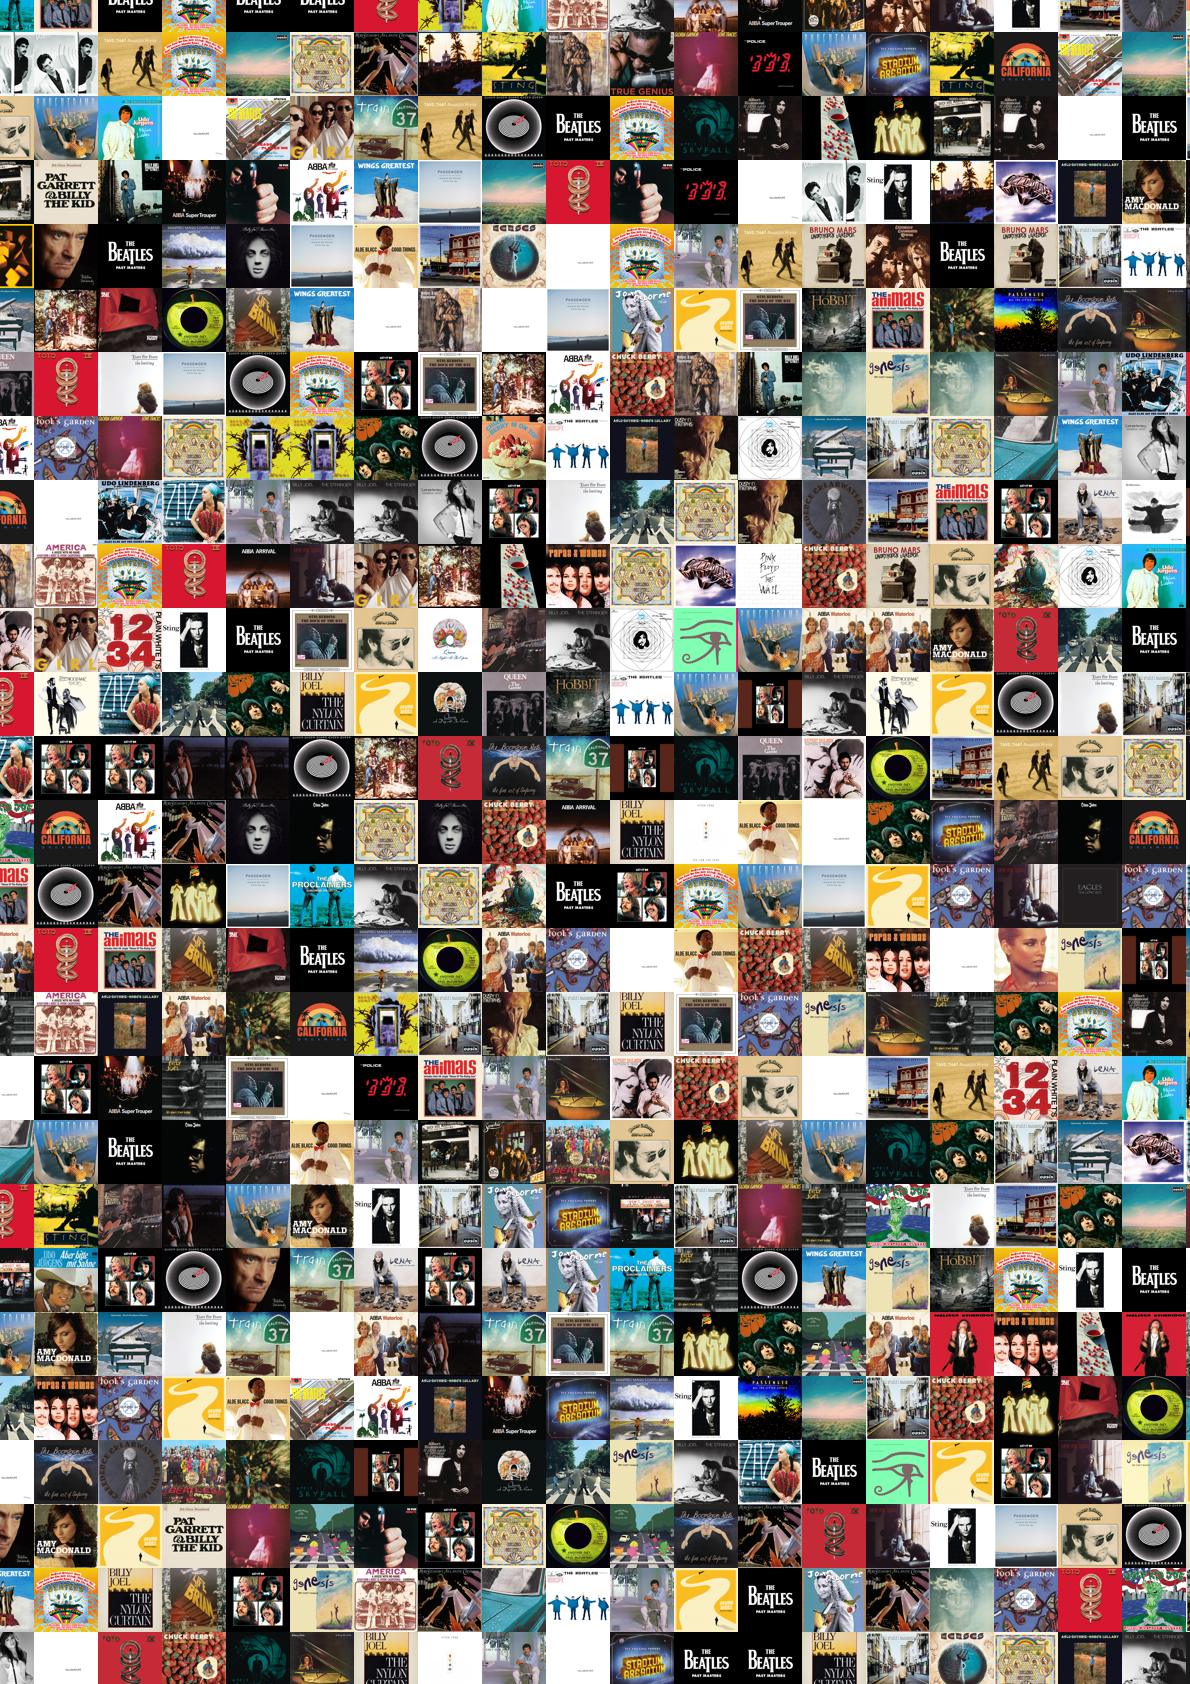
\includegraphics[width=\paperwidth]{cover_background.png}};
    \vspace{10cm}

    \begin{center}
        {
            \fontsize{80}{96}
            \selectfont
            \contour{black}{\protect\color{white}Songbook}
        }
        ~\\
        {
            \fontsize{40}{50}
            \selectfont
            \contour{black}{\protect\color{white}Niklas}
        }
    \end{center}
    \newpage
    \tableofcontents
    \newpage
    \pagestyle{plain}
    \pagenumbering{arabic}
    \setcounter{page}{1}
    \invisiblesection{(Sittin' On) the Dock of the Bay~~~{\footnotesize Otis Redding}}

    \begin{center}
        \textbf{(Sittin' On) the Dock of the Bay}
        ~\\
        Otis Redding -- The Dock of the Bay (1968)
    \end{center}
    {
        \scriptsize
        \textbf{Verse 1}
        ~\\
        {
            \cutive
            \obeyspaces
G                      B7
\\
Sitting in the morning sun
\\
        C                        A
\\
I'll be sitting when the evening comes
\\
G                       B7
\\
Watching the ships roll in
\\
             C                       A
\\
Then I'll be watching them roll away again
\\

        }
        \textbf{Chorus}
        ~\\
        {
            \cutive
            \obeyspaces
G                          E
\\
Sitting on the dock of the bay
\\
             G          E
\\
Watching the tide roll away
\\
G                          A
\\
Sitting at the dock of the bay
\\
        G   E
\\
Wasting time 
\\

        }
        \textbf{Verse 2}
        ~\\
        {
            \cutive
            \obeyspaces
G                 B7
\\
I left my home in Georgia
\\
C                     A
\\
Headed for the Frisco Bay
\\
  G              B7
\\
I had nothing to live for
\\
           C                     A
\\
Looks like nothing gonna come my way
\\

        }
        \textbf{Chorus}
        ~\\
        {
            \cutive
            \obeyspaces

        }
        \textbf{Bridge}
        ~\\
        {
            \cutive
            \obeyspaces
G         D C               G
\\
Looks like  nothing's gonna change
\\
G          D       C         G
\\
Everything still remains the same
\\
G       D                  C          G
\\
I can't do what ten people tell me to do
\\
F                          D
\\
So I guess I'll remain the same, check it
\\

        }
        \textbf{Verse 3}
        ~\\
        {
            \cutive
            \obeyspaces
G                       B7
\\
Sitting here resting my bones
\\
        C                         A
\\
And the loneliness won't leave me alone
\\
G                    B7
\\
Two thousand miles I roam
\\
        C                 A
\\
Just to make this dock my home
\\

        }
        \textbf{Chorus}
        ~\\
        {
            \cutive
            \obeyspaces

        }
    }
    \pagebreak
    \invisiblesection{1, 2, 3, 4~~~{\footnotesize Plain White T’s}}

    \begin{center}
        \textbf{1, 2, 3, 4}
        ~\\
        Plain White T's -- 1, 2, 3, 4 (2008)
    \end{center}
    {
        \scriptsize
        \textbf{Verse 1}
        ~\\
        {
            \cutive
            \obeyspaces
D
\\
Give me more lovin' than I've ever had
\\
A
\\
Make it all better when I'm feelin' sad
\\
Bm                                         A
\\
Tell me that I'm special even when I know I'm not
\\
D
\\
Make me feel good when I hurt so bad
\\
A                                      Bm
\\
Barely gettin' mad, I'm so glad I found you
\\
                A
\\
I love bein' around you
\\
             G                  A
\\
You make it easy, it's as easy as 1, 2, 1, 2, 3, 4
\\

        }
        \textbf{Chorus}
        ~\\
        {
            \cutive
            \obeyspaces
             D        A
\\
There's only one thing to do
\\
  Bm         A    G  Gm  D
\\
Three words for you I love you
\\
             D        A
\\
There's only one way to say
\\
      Bm               A                G Gm D
\\
Those three words and that's what I'll do, I love you
\\

        }
        \textbf{Verse 2}
        ~\\
        {
            \cutive
            \obeyspaces
D
\\
Give me more lovin' from the very start
\\
A
\\
Piece me back together when I fall apart
\\
Bm                                                A
\\
Tell me things you never even tell your closest friends
\\
D
\\
Make me feel good when I hurt so bad
\\
A                                      Bm
\\
Best that I've had, I'm so glad that I found you
\\
                A
\\
I love bein' around you
\\
             G                  A
\\
You make it easy, it's as easy as 1, 2, 1, 2, 3, 4
\\

        }
        \textbf{Chorus}
        ~\\
        {
            \cutive
            \obeyspaces

        }
        \textbf{Solo Verse}
        ~\\
        {
            \cutive
            \obeyspaces
G                  A
\\
You make it easy, it's easy as 1, 2, 1, 2, 3, 4
\\

        }
        \textbf{Chorus}
        ~\\
        {
            \cutive
            \obeyspaces

        }
        \textbf{Outro}
        ~\\
        {
            \cutive
            \obeyspaces
D A Bm A G Gm D
\\
        I love you
\\
D A Bm A G Gm D
\\
1, 2, 3, 4 I love you
\\
G Gm D
\\
I love you\\

        }
    }
    \pagebreak
    \invisiblesection{A Horse With No Name~~~{\footnotesize America}}

    \begin{center}
        \textbf{A Horse With No Name}
        ~\\
        America -- America (1971)
    \end{center}
    {
        \footnotesize
        \textbf{Verse 1}
        ~\\
        {
            \cutive
            \obeyspaces
       Em                D6/9
\\
On the first part of the journey
\\
       Em                D6/9
\\
I was lookin at all the life
\\
            Em                 D6/9
\\
There were plants and birds and rocks and things
\\
            Em                D6/9
\\
There were sand and hills and rings
\\
       Em                  D6/9
\\
The first thing I met was a fly with a buzz
\\
         Em           D6/9
\\
and the sky with no clouds
\\
     Em                   D6/9
\\
the heat was hot and the ground was dry
\\
         Em              D6/9
\\
but the air was full of sound
\\

        }
        \textbf{Chorus}
        ~\\
        {
            \cutive
            \obeyspaces
      Em9                         Dmaj9
\\
I've been through the desert on a horse with no name
\\
        Em9                   Dmaj9
\\
it felt good to be out of the rain
\\
       Em9           Dmaj9
\\
in the desert you can remember your name
\\
              Em9                Dmaj9
\\
'cause there ain't no one for to give you no pain
\\
   Em9    Dmaj9
\\
La la   la la lala la lala   
\\
Em9    Dmaj9
\\
la la la 
\\

        }
        \textbf{Verse 2}
        ~\\
        {
            \cutive
            \obeyspaces
       Em                D6/9
\\
After two days in the desert sun
\\
    Em                D6/9
\\
my skin began to turn red
\\
       Em              D6/9
\\
After three days in the desert fun
\\
       Em                D6/9
\\
I was looking at a river bed
\\
        Em                D6/9
\\
And the story it told of a river that flowed
\\
       Em                 D6/9
\\
made me sad to think it was dead
\\

        }
        \textbf{Chorus}
        ~\\
        {
            \cutive
            \obeyspaces

        }
        \textbf{Verse 3}
        ~\\
        {
            \cutive
            \obeyspaces
       Em                D6/9
\\
After nine days I let the horse run free
\\
            Em                D6/9
\\
'cause the desert had turned to sea
\\
            Em                  D6/9
\\
there were plants and birds and rocks and things
\\
             Em                D6/9
\\
there were sand and hills and rings
\\
      Em                        D6/9
\\
The ocean is a desert with it's life underground
\\
          Em              D6/9
\\
and the perfect disguise above
\\
            Em           D6/9
\\
Under the cities lies a heart made of ground
\\
         Em                 D6/9
\\
but the humans will give no love
\\

        }
        \textbf{Chorus}
        ~\\
        {
            \cutive
            \obeyspaces

        }
    }
    \pagebreak
    \invisiblesection{Aber bitte mit Sahne~~~{\footnotesize Udo Jürgens}}

    \begin{center}
        \textbf{Aber bitte mit Sahne}
        ~\\
        Udo Jürgens -- Aber bitte mit Sahne (1976)
    \end{center}
    {
        \scriptsize
        \textbf{Verse 1}
        ~\\
        {
            \cutive
            \obeyspaces
C                                                 F (Bbsus2 F)      C (F C)
\\
Sie treffen sich taeglich um viertel nach drei  aaahh          ooojehh
\\
                                           F (Bbsus2 F)      C (F C)
\\
am Stammtisch im Eck in der Konditorei  aaahh          ooojehh
\\
    F                        C
\\
und blasen zum Sturm auf das Kuchenbuffett
\\
    F                            G
\\
auf Schwarzwaelder Kirsch und auf Sahnebaiser
\\
    C           C7      F          F7    F F\# G
\\
auf Fruechteeis, Ananas, Kirsch und Banane
\\
               C (F C)                C (F C)
\\
aber bitte mit Sahne, aber bitte mit Sahne...
\\

        }
        \textbf{Verse 2}
        ~\\
        {
            \cutive
            \obeyspaces
C                                                   F (Bbsus2 F)      C (F C)
\\
Sie schwatzen und schmatzen, dann holen sie sich aaahh          ooojehh
\\
                                         F (Bbsus2 F)      C (F C)
\\
noch Buttercremetorte und Bienenstich aaahh          ooojehh
\\
    F                        C
\\
sie pusten und prusten, fast geht nichts mehr rein,
\\
        F                          G
\\
nur ein Mohrenkopf hoechstens, denn Ordnung muss sein
\\
    C         C7       F         F7      F F\# G
\\
Bei Mathilde, Ottilie, Marie und Liliane
\\
               C (F C)                C (F C)
\\
aber bitte mit Sahne, aber bitte mit Sahne...
\\

        }
        \textbf{Verse 3}
        ~\\
        {
            \cutive
            \obeyspaces
C                                               F (Bbsus2 F)     C (F C)
\\
Und das Ende vom Lied hat wohl jeder geahnt, aaahh          ooojehh
\\
C                                        F (Bbsus2 F)     C (F C)
\\
der Tod hat reihum sie dort abgesahnt aaahh          ooojehh
\\
          F                    C
\\
die Hinterbliebenen fanden vor Schmerz keine Worte,
\\
    F                        G
\\
mit Sacher- und Linzer - und Marzipantorte
\\
          C        C7         F             F7   F F\# G
\\
hielt als letzte Liliane geht treu noch zur Fahne
\\
               C (F C)               C (F C)
\\
aber bitte mit Sahne, aber bitte mit Sahne...
\\

        }
        \textbf{Verse 4}
        ~\\
        {
            \cutive
            \obeyspaces
C                                                  F (Bbsus2 F)     C (F C)
\\
Doch auch mit Liliane war es schliesslich vorbei aaahh          ooojehh
\\
                                          F (Bbsus2 F)     C (F C)
\\
sie kippte vom Stuhl in der Konditorei hmmmm          ooojehh
\\
        F                         C
\\
auf dem Sarg gabs statt Kraenze verzuckerte Torten
\\
       F                      G
\\
und er Pfarrer begrub sie mit ruehrenden Worten
\\
         C            C7         F          F7    F F\# G
\\
dass der Herrgott den Weg in den Himmel ihr bahne
\\
               C (F C)                C (F C)
\\
aber bitte mit Sahne, aber bitte mit Sahne...
\\
                  C                      C (F C)
\\
noch ein Taesschen Kaffee, aber bitte mit Sahne
\\
                 C                      C (F C)
\\
noch ein kleines Baiser, aber bitte mit Sahne
\\
                                 C                      C (F C)
\\
oder solls vieleicht doch ein Keks sein? aber bitte mit Sahne...\\

        }
    }
    \pagebreak
    \invisiblesection{Across the Universe~~~{\footnotesize The Beatles}}

    \begin{center}
        \textbf{Across the Universe}
        ~\\
        The Beatles -- Across the Universe (1969)
         -- Capo 1
    \end{center}
    {
        \scriptsize
        \textbf{Verse 1}
        ~\\
        {
            \cutive
            \obeyspaces
D                 Bm               F\#m
\\
Words are flowing out like endless rain into a paper cup
\\
     Em7                          A              A7
\\
They slither wildly as they slip away across the universe
\\
D                Bm               F\#m
\\
Pools of sorrow, waves of joy are drifting through my opened mind
\\
  Em7            Gm
\\
Possessing and caressing me
\\

        }
        \textbf{Chorus}
        ~\\
        {
            \cutive
            \obeyspaces
D             A7sus4
\\
Jai guru deva om
\\
A                         A7
\\
Nothing's gonna change my world
\\
G                         D
\\
Nothing's gonna change my world
\\
A                         A7
\\
Nothing's gonna change my world
\\
G                         D
\\
Nothing's gonna change my world
\\

        }
        \textbf{Verse 2}
        ~\\
        {
            \cutive
            \obeyspaces
D         Bm                 F\#m                            Em7
\\
Images of broken light which dance before me like a million eyes
\\
                        A            A7
\\
They call me on and on across the universe
\\
D                Bm              F\#m
\\
Thoughts meander like a restless wind inside a letterbox
\\
     Em7                               A              A7
\\
They tumble blindly as they make their way across the universe
\\

        }
        \textbf{Chorus}
        ~\\
        {
            \cutive
            \obeyspaces

        }
        \textbf{Verse 3}
        ~\\
        {
            \cutive
            \obeyspaces
D                   Bm                 F\#m
\\
Sounds of laughter, shades of life are ringing through my opened ears
\\
  Em7          Gm
\\
Inciting and inviting me
\\
D            Bm               F\#m                             Em7
\\
Limitless, undying love which shines around me like a million suns
\\
                        A            A7
\\
And calls me on and on across the universe
\\

        }
        \textbf{Chorus}
        ~\\
        {
            \cutive
            \obeyspaces

        }
    }
    \pagebreak
    \invisiblesection{Africa~~~{\footnotesize Toto}}

    \begin{center}
        \textbf{Africa}
        ~\\
        Toto -- TOTO IV (1982)
         -- Capo 3
    \end{center}
    {
        \scriptsize
        \textbf{Verse 1}
        ~\\
        {
            \cutive
            \obeyspaces
D                   F\#m     Bm
\\
I hear the drums echoing tonight
\\
D/A              C/G           Em         Bm   C Bm Em
\\
She hears only whispers of some quiet conversa - tion
\\
D                 F\#m           Bm
\\
She's coming in, twelve thirty flight
\\
D/A              C/G                    Em7              Bm   C Bm Em
\\
The moonlit wings reflect the stars that guide me toward salva-tion
\\
D              F\#m             Bm
\\
I stopped an old man along the way
\\
D/A                C/G            Em              Bm   C Bm Em
\\
Hoping to find some old forgotten words or ancient melo-dies
\\
D              F\#m       Bm                  C                Em
\\
He turned to me as if to say "hurry boy, it's waiting there for you"
\\

        }
        \textbf{Chorus}
        ~\\
        {
            \cutive
            \obeyspaces
Am          F               C        G
\\
Gonna take a lot to drag me away from you
\\
Am                     F             C               G
\\
There's nothing that a hundred men or more could ever do
\\
Am          F           C   G
\\
I bless the rains down in  Africa
\\
Am             F               C              Em G Am G C
\\
Gonna take some time to do the things we never had...
\\
    C Bm Em
\\
Ooo Ooo
\\
    C Bm Em
\\

        }
        \textbf{Verse 2}
        ~\\
        {
            \cutive
            \obeyspaces
D             F\#m            Bm
\\
The wild dogs cry out in the night
\\
D/A                  C/G              Em      Bm   C Bm Em
\\
As they grow restless longing for some solitary compa-ny
\\
D           F\#m              Bm
\\
I know that I must do what's right
\\
D/A                   C/G        Em               Bm    C Bm Em
\\
As sure as Kilimanjaro rises like Olympus above the Serengeti
\\
D         F\#m                Bm
\\
I seek to cure what's deep inside
\\
Bm                C                   Em
\\
Frightened of this thing that I've become
\\

        }
        \textbf{Chorus}
        ~\\
        {
            \cutive
            \obeyspaces

        }
        \textbf{Interlude}
        ~\\
        {
            \cutive
            \obeyspaces
D   F\#m  Bm
\\
D   C    Em  Bm   C Bm Em
\\
D   F\#7  Bm                 C                  Em
\\
            "hurry boy, she's waiting there for you"
\\

        }
        \textbf{Outro/Chorus}
        ~\\
        {
            \cutive
            \obeyspaces
     Am          F               C        G
\\
It's gonna take a lot to drag me away from you
\\
Am                    F              C               G
\\
There's nothing that a hundred men or more could ever do
\\
Am        F             C   G
\\
I bless the rains down in  Africa
\\
Am        F             C   G
\\
I bless the rains down in  Africa
\\
Am        F             C   G
\\
I bless the rains down in  Africa
\\
Am        F             C   G
\\
I bless the rains down in  Africa
\\
Am        F             C   G
\\
I bless the rains down in  Africa
\\
Am             F               C              Em G Am  G C
\\
Gonna take some time to do the things we never had...
\\
    C Bm Em
\\
Ooo Ooo
\\
    (repeat fading)
\\
    C Bm Em\\

        }
    }
    \pagebreak
    \invisiblesection{All You Need Is Love~~~{\footnotesize The Beatles}}

    \begin{center}
        \textbf{All You Need Is Love}
        ~\\
        The Beatles -- Magical Mystery Tour (1967)
    \end{center}
    {
        \scriptsize
        \textbf{Verse 1}
        ~\\
        {
            \cutive
            \obeyspaces
G                        D                Em
\\
 There's nothing you can do that can't be done
\\
G                D                  Em
\\
 Nothing you can sing that can't be sung
\\
Am               G                     D
\\
 Nothing you can say but you can learn how to play the game,
\\
      1 + 2 + 3 + 4 + 1 + 2 + 3 +
\\
      D       D7      D6      D
\\
 It's easy
\\

        }
        \textbf{Verse 2}
        ~\\
        {
            \cutive
            \obeyspaces
G                        D                  Em
\\
 There's nothing you can make that can't be made
\\
G             D               Em
\\
 No one you can save that can't be saved.
\\
Am               G               D
\\
 Nothing you can do but you can learn how to be you in time,
\\
      1 + 2 + 3 + 4 + 1 + 2 + 3 +
\\
      D       D7      D6      D
\\
 It's easy
\\

        }
        \textbf{Chorus}
        ~\\
        {
            \cutive
            \obeyspaces
G        A        D     D7
\\
All you need is love
\\
G        A        D     D7
\\
All you need is love
\\
G        B7      Em   G    C       D       G
\\
All you need is love love, Love is all you need.
\\

        }
        \textbf{Instrumental Verse}
        ~\\
        {
            \cutive
            \obeyspaces

        }
        \textbf{Chorus}
        ~\\
        {
            \cutive
            \obeyspaces

        }
        \textbf{Verse 3}
        ~\\
        {
            \cutive
            \obeyspaces
G                        D               Em
\\
 There's nothing you can know that isn't known.
\\
G                D              Em
\\
 Nothing you can see that isn't shown.
\\
Am               G              D
\\
 Nowhere you can be that isn't where you're meant to be,
\\
      1 + 2 + 3 + 4 + 1 + 2 + 3 +
\\
      D       D7      D6      D
\\
 It's easy
\\

        }
        \textbf{Chorus x2}
        ~\\
        {
            \cutive
            \obeyspaces

        }
    }
    \pagebreak
    \invisiblesection{Allentown~~~{\footnotesize Billy Joel}}

    \begin{center}
        \textbf{Allentown}
        ~\\
        Billy Joel -- The Nylon Curtain (1982)
    \end{center}
    {
        \scriptsize
        \textbf{Verse 1}
        ~\\
        {
            \cutive
            \obeyspaces
A          Em             A    D
\\
Well we're living here in Allentown
\\
            Am              D         G
\\
And they're closing all the factories down
\\
       Em                A       Bm
\\
Out in Bethlehem they're killing time
\\
A           Em
\\
Filling out forms
\\
D           A
\\
Standing in line.
\\
         Em                 A            D
\\
Well our fathers fought the Second World War
\\
            Am              D      G
\\
Spent their weekends on the Jersey Shore
\\
        Em             A Bm  A
\\
Met our mothers at the USO
\\
A             Em
\\
Asked them to dance
\\
D                A   A7
\\
Danced with them slow
\\
          Em             A    D
\\
And we're living here in Allentown.
\\
        F                G      C
\\
But the restlessness was handed down
\\
         Am           D       Em                    Bm       C D G
\\
And it's getting very hard to staaaaaaaaaaaaaaaaaaaaaaaaaaaay
\\
C D G 2x
\\

        }
        \textbf{Verse 2}
        ~\\
        {
            \cutive
            \obeyspaces
A          Em              A    D
\\
Well we're waiting here in Allentown
\\
        Am           D        G
\\
For the Pennsylvania we never found
\\
        Em           A        Bm
\\
For the promises our teachers gave
\\
A            Em
\\
If we worked hard
\\
D       A    A7
\\
If we behaved.
\\
       Em          A           D
\\
So the graduations hang on the wall
\\
         Am           D            G
\\
But they never really helped us at all
\\
        Em              A        Bm
\\
No they never taught us what was real
\\
A       Em
\\
Iron or coke,
\\
D        A    A7
\\
Chromium steel.
\\
          Em              A    D
\\
And we're waiting here in Allentown.
\\
            F             G             C
\\
But they've taken all the coal from the ground
\\
        Am           D       Em          Bm       C D G
\\
And the union people crawled awaaaaaaaaaaaaaaaaaaay
\\
C D G 2x
\\

        }
        \textbf{Bridge}
        ~\\
        {
            \cutive
            \obeyspaces
F                 G           F
\\
Every child had a pretty good shot
\\
          G               F             Bb
\\
To get at least as far as their old man got.
\\
F                            G           F
\\
If something happened on the way to that place
\\
                            G          F G
\\
They threw an American flag in our face, 
\\
C D G 2x
\\

        }
        \textbf{Verse 3}
        ~\\
        {
            \cutive
            \obeyspaces
A        Em             A    D
\\
Well I'm living here in Allentown
\\
         Am             D        G
\\
And it's hard to keep a good man down.
\\
      Am               D    Em           Bm           C D G
\\
But I won't be getting up todaaaaaaaaaaaaaaaaaayyyyyyyy
\\
C D G
\\

        }
        \textbf{Solo Bridge}
        ~\\
        {
            \cutive
            \obeyspaces

        }
        \textbf{Outro}
        ~\\
        {
            \cutive
            \obeyspaces
         Am           D       Em       Bm     C D G
\\
And it's getting very hard to staaaaaaaaaaaaaay.
\\
          Am             D    G     C G
\\
And we're living here in Allentown.\\

        }
    }
    \pagebreak
    \invisiblesection{Always Look on the Bright Side of Life~~~{\footnotesize Monty Python}}

    \begin{center}
        \textbf{Always Look on the Bright Side of Life}
        ~\\
        Monty Python -- Monty Python's Life of Brian (1979)
    \end{center}
    {
        \scriptsize
        \textbf{Verse 1}
        ~\\
        {
            \cutive
            \obeyspaces
     Am                 D             G               Em
\\
Some things in life are bad, they can really make you mad
\\
      Am                   D         G
\\
Other things just make you swear and curse
\\
            Am                D
\\
When you're chewing on life's gristle
\\
      G               Em
\\
Don't grumble, give a whistle
\\
    A7                                   D7
\\
And this'll help things turn out for the best
\\

        }
        \textbf{Chorus}
        ~\\
        {
            \cutive
            \obeyspaces

        }
        \textbf{Verse 2}
        ~\\
        {
            \cutive
            \obeyspaces
   Am               D               G                Em
\\
If life seems jolly rotten, there's something you've forgotten
\\
              Am                  D         G
\\
and that's to laugh and smile and dance and sing.
\\
            Am             D               G     Em
\\
When you're feeling in the dumps, don't be silly chumps
\\
     A7                                       D7
\\
Just purse your lips and whistle - that's the thing
\\

        }
        \textbf{Chorus}
        ~\\
        {
            \cutive
            \obeyspaces

        }
        \textbf{Verse 3}
        ~\\
        {
            \cutive
            \obeyspaces
     Am               D        G               Em
\\
For life is quite absurd and death's the final word
\\
         Am              D              G
\\
You must always face the curtain with a bow
\\
   Am             D              G          Em
\\
Forget about your sin - give the audience a grin
\\
  A7                                D7
\\
Enjoy it - it's your last chance anyhow.
\\

        }
        \textbf{Chorus}
        ~\\
        {
            \cutive
            \obeyspaces
    G      Em          Am     D7      G      Em    Am    D7
\\
So always look on the bright side of death
\\
G      Em       Am           D7    G         Em    Am    D7
\\
Just before you draw your terminal breath
\\

        }
        \textbf{Verse 4}
        ~\\
        {
            \cutive
            \obeyspaces
Am                D    G                Em
\\
Life's a piece of shit when you look at it
\\
Am                 D                    G
\\
Life's a laugh and death's a joke, it's true
\\
       Am             D
\\
You'll see it's all a show,
\\
         G               Em
\\
keep 'em laughing as you go
\\
       A7                               D7
\\
Just remember that the last laugh is on you
\\

        }
        \textbf{Chorus}
        ~\\
        {
            \cutive
            \obeyspaces

        }
        \textbf{Outro x4}
        ~\\
        {
            \cutive
            \obeyspaces
    A      F\#m         Bm     E7      A     F\#m   Bm    E7
\\
And always look on the bright side of life\\

        }
    }
    \pagebreak
    \invisiblesection{American Pie~~~{\footnotesize Don McLean}}

    \begin{center}
        \textbf{American Pie}
        ~\\
        Don McLean -- American Pie (1971)
    \end{center}
    {
        \scriptsize
        \textbf{Verse 1}
        ~\\
        {
            \cutive
            \obeyspaces
  G     D/F\#    Em7
\\
A long, long time ago,
\\
Am            C                  Em                  D
\\
I can still remember how that music used to make me smile
\\
    G      D/F\#   Em7
\\
And I knew if I had my chance,
\\
     Am                 C                Em              C            D
\\
That I could make those people dance and maybe they'd be happy for a while
\\
    Em       Am              Em                 Am
\\
But February made me shiver, with every paper I'd deliver
\\
C        G/B    Am             C                     D
\\
Bad news on the doorstep, I couldn't take one more step
\\
  G          D/F\#     Em           Am7            D
\\
I can't remember if I cried when I read about his widowed bride
\\
G         D/F\#       Em
\\
Something touched me deep inside
\\
    C      D7      G
\\
The day the music died
\\

        }
        \textbf{Chorus}
        ~\\
        {
            \cutive
            \obeyspaces
   G    C        G        D
\\
So bye, bye Miss American Pie
\\
         G            C            G        D
\\
Drove my Chevy to the levy but the levy was dry
\\
         G        C                  G           D
\\
And them good old boys were drinkin' whiskey and rye
\\
Em*                         A7*   Em*                         D7
\\
this will be the day that I die, this will be the day that I die
\\

        }
        \textbf{Verse 2}
        ~\\
        {
            \cutive
            \obeyspaces
G                 Am
\\
Did you write the book of love
\\
       C                 Am         Em           D
\\
And do you have faith in god above, if the bible tells you so?
\\
G      D/F\#        Em
\\
Do you believe in rock and roll
\\
    Am7            C              Em                 A7           D
\\
Can music save your mortal soul and can you teach me how to dance real slow?
\\
       Em*                  D*                   Em*             D*
\\
Well I know that you're in love with him 'cuz I saw you dancin' in the gym
\\
    C           G/B      A7           C                    D7
\\
You both kicked off your shoes, man I dig those rhythm and blues
\\
        G      D/F\#     Em                   Am                   C
\\
I was a lonely teenage bronckin' buck with a pink carnation and a pickup truck
\\
    G     D/F\#    Em              C       D7    G  C  G
\\
But I knew I was out of luck the day the music died, I started singin'
\\

        }
        \textbf{Chorus}
        ~\\
        {
            \cutive
            \obeyspaces

        }
        \textbf{Verse 3}
        ~\\
        {
            \cutive
            \obeyspaces
         G                   Am
\\
Now for ten years we've been on our own,
\\
      C                   Am          Em                     D
\\
and moss grows fat on a rolling stone but that's not how it used to be
\\
          G     D/F\#            Em
\\
When the jester sang for the king and queen 
\\
     Am7                C                   Em             A7          D
\\
in a coat he borrowed from James Dean in a voice that came from you and me
\\
         Em*                 D*               Em*                 D*
\\
Oh, and while the king was looking down, the jester stole his thorny crown
\\
     C        G/B   A7       C                D7
\\
The courtroom was adjourned, no verdict was returned
\\
          G         D/F\#  Em             Am           C
\\
And while Lennon read a book on Marx, the quartet practiced in the park
\\
    G        D/F\#   Em             C         D7     G  C  G
\\
And we sang dirges in the dark the day the music died, we were singin'
\\

        }
        \textbf{Chorus}
        ~\\
        {
            \cutive
            \obeyspaces

        }
        \pagebreak
        \textbf{Verse 4}
        ~\\
        {
            \cutive
            \obeyspaces
G                   Am
\\
Helter skelter in a summer swelter
\\
C                      Am                 Em                     D
\\
the birds flew off with a fallout shelter, eight miles high and fallin' fast
\\
      G   D/F\#  Em
\\
It landed foul on the grass
\\
      Am7                C            Em                             A7     D
\\
the players tried for a forward pass, with the jester on the sidelines in a cast
\\
         Em*               D*                  Em*                 D*
\\
Now the half-time air was sweet perfume, while sergeants played a marching tune
\\
C          G/B      A7      C                  D7
\\
We all got up to dance, but we never got the chance
\\
          G      D/F\#      Em                 Am              Cm
\\
'Cuz the players tried to take the field, the marching band refused to yield
\\
    G    D/F\#       Em              C        D7       G  C  G
\\
Do you recall what was revealed the day the music died,    we started singin'
\\

        }
        \textbf{Chorus}
        ~\\
        {
            \cutive
            \obeyspaces

        }
        \textbf{Verse 5}
        ~\\
        {
            \cutive
            \obeyspaces
     G                Am
\\
And there we were all in one place,
\\
    C        Am            Em                   D
\\
a generation lost in space, with no time left to start again
\\
            G      D/F\#   Em               Am7                 C
\\
So come on Jack be nimble, Jack be quick, Jack Flash sat on a candle 
\\
       Em                   A7             D
\\
stick, 'cuz fire is the devil's only friend
\\
     Em*              D*               Em*                    D*
\\
And as I watched him on the stage, my hands were clenched in fists of rage
\\
   C      G/B    A7         C                  D7
\\
No angel born in Hell could break that Satan's spell
\\
           G            D/F\#      Em             Am              C
\\
And as the flames climbed high into the night to light the sacrificial rite
\\
       G   D/F\#           Em           C      D7      G  C  G
\\
I saw Satan laughing with delight the day the music died,     he was singin'
\\

        }
        \textbf{Chorus}
        ~\\
        {
            \cutive
            \obeyspaces

        }
        \textbf{Verse 6}
        ~\\
        {
            \cutive
            \obeyspaces
  G    D/F\#       Em
\\
I met a girl who sang the blues
\\
      Am                 C               Em                      D
\\
And I asked her for some happy news, but she just smiled and turned away
\\
  G       D/F\#      Em
\\
I went down to the sacred store
\\
       Am              C                     Em                 C
\\
Where I'd heard the music years before, but the man there said the music
\\
         D
\\
wouldn't play
\\
    Em*                Am*                    Em*                  Am*
\\
But in the streets the children screamed, the lovers cried and the poets dreamed
\\
    C     G/B      Am          C                     D
\\
But not a word was spoken, the church bells all were broken
\\
        G       D/F\#   Em            Am7     C             D7
\\
And the three men I admire most, the Father, Son, and the Holy Ghost
\\
G             D/F\#          Em               C       D7    G
\\
They caught the last train for the coast the day the music died,
\\
N.C.
\\
And they were singin'
\\

        }
        \textbf{Chorus x2}
        ~\\
        {
            \cutive
            \obeyspaces

        }
    }
    \pagebreak
    \invisiblesection{Another Brick in the Wall~~~{\footnotesize Pink Floyd}}

    \begin{center}
        \textbf{Another Brick in the Wall}
        ~\\
        Pink Floyd -- The Wall (2004)
    \end{center}
    {
        \scriptsize
        \textbf{Verse x2}
        ~\\
        {
            \cutive
            \obeyspaces
Dm
\\
We don't need no education! We don't need no thought control! 
\\
Dm                                                          G
\\
No dark sarcasm in the class room! Teacher leave those kids alone!
\\
G                                 Dm
\\
Hey! Teacher! Leave them kids alone!
\\
F                    C                        Dm
\\
All in all it's just another brick in the wall!
\\
All in all you're just another brick in the wall!\\

        }
    }
    \pagebreak
    \invisiblesection{Another Day~~~{\footnotesize Paul McCartney}}

    \begin{center}
        \textbf{Another Day}
        ~\\
        Paul McCartney -- Another Day / Oh Woman Oh Why (1971)
    \end{center}
    {
        \scriptsize
        \textbf{Verse 1}
        ~\\
        {
            \cutive
            \obeyspaces
      G                                 B7
\\
Every day she takes a morning bath, she wets her hair,
\\
Em                                Am
\\
wraps a towel around her as she's heading for the bedroom chair.
\\
          D7       G
\\
It's just another day.
\\
C             G          C             G
\\
Slipping into stockings, stepping into shoes,
\\
C              G              A
\\
dipping in the pocket of her raincoat.
\\
D7                   G
\\
  It's just another day.
\\

        }
        \textbf{Verse 2}
        ~\\
        {
            \cutive
            \obeyspaces
       G                                 B7
\\
At the office where the papers grow, she takes a break,
\\
Em                            Am
\\
drinks another coffee and she finds it hard to stay awake.
\\
          D7       G
\\
It's just another day.
\\

        }
        \textbf{Chorus}
        ~\\
        {
            \cutive
            \obeyspaces
C                   Am          D7       G
\\
 Du du du, du du, du, it's just another day.
\\
          E7       Am          D7       G
\\
Du du du, du du, du, it's just another day.
\\
G  D7  Em
\\

        }
        \textbf{Bridge}
        ~\\
        {
            \cutive
            \obeyspaces
   Em      Cmaj7 Em6/C\#         Cmaj7   Em
\\
So sad, so sad,  sometimes she feels so sad.
\\
 Em                          Cmaj7
\\
Alone in her apartment she'd dwell
\\
                    Em6/C\#           Cmaj7    Em     Fill
\\
till the man of her dreams comes to break the spell.
\\
E   Am7                   D
\\
Ah, stay, don't stand her up.
\\
       Daug         Bm/D         B7              Em
\\
And he comes and he stays but he leaves the next day.
\\
   C    Em6/C\#         Cmaj7   Em
\\
So sad, sometimes she feels so sad.
\\

        }
        \textbf{Verse 3}
        ~\\
        {
            \cutive
            \obeyspaces
       G                           B7
\\
As she posts another letter to the sound of five,
\\
Em                              Am
\\
people gather round her and she finds it hard to stay alive.
\\
          D7       G
\\
It's just another day.
\\

        }
        \textbf{Chorus}
        ~\\
        {
            \cutive
            \obeyspaces

        }
        \textbf{Bridge}
        ~\\
        {
            \cutive
            \obeyspaces

        }
        \textbf{Verse 1}
        ~\\
        {
            \cutive
            \obeyspaces

        }
        \textbf{Chorus}
        ~\\
        {
            \cutive
            \obeyspaces

        }
    }
    \pagebreak
    \invisiblesection{Anywhere~~~{\footnotesize Passenger}}

    \begin{center}
        \textbf{Anywhere}
        ~\\
        Passenger -- Young as the Morning Old as the Sea (2016)
    \end{center}
    {
        \scriptsize
        \textbf{Verse 1}
        ~\\
        {
            \cutive
            \obeyspaces
G           D          G
\\
 If you get out on the ocean
\\
Cadd9        Em7        D
\\
 If you sail out on the sea
\\
G           D         G
\\
 If you get up in the mountains
\\
Cadd9      Em7         D
\\
 If you go climbing on trees
\\
G              D      G
\\
 Oh through every emotion
\\
Cadd9               Em7        D
\\
 When you know that they don't care
\\
G                D        G
\\
 Darling, that's when I'm with you
\\
Cadd9    Em7         D
\\
 Oh I'll go with you anywhere
\\

        }
        \textbf{Verse 2}
        ~\\
        {
            \cutive
            \obeyspaces
If you get up in a jet plane
\\
Or down in a submarine
\\
If you get onto the next train
\\
To somewhere you never been
\\
If you wanna ride in a fast car
\\
And feel the wind in your hair
\\
Darling just look beside you
\\
Oh I'll go with you anywhere
\\

        }
        \textbf{Instrumental}
        ~\\
        {
            \cutive
            \obeyspaces

        }
        \textbf{Chorus}
        ~\\
        {
            \cutive
            \obeyspaces
Cadd9      Em7
\\
 Oh and I will be with you
\\
D         G       D
\\
 When the darkest winter comes
\\
Cadd9     Em7
\\
 Oh and I will be with you
\\
D            G      D   Cadd9
\\
 To feel the California sun      
\\
         Em7
\\
 Oh and I will be with you
\\
B7      Em7       D          Cadd9
\\
 In the nighttime when it's through
\\
D
\\
 Oh I'll go anywhere with you
\\

        }
        \textbf{Verse 3}
        ~\\
        {
            \cutive
            \obeyspaces
If you get up in the hillside
\\
If you ride out on the plains
\\
If you go digging up dirt
\\
If you go out dancing in the rain
\\
If you go chasing them rainbows
\\
Just to find the gold ain't there
\\
Darling just look behind you
\\
Oh I'll go with you anywhere
\\

        }
        \textbf{Chorus}
        ~\\
        {
            \cutive
            \obeyspaces

        }
        \textbf{Instrumental}
        ~\\
        {
            \cutive
            \obeyspaces
Em7 D Cadd9 G x2
\\

        }
        \textbf{Chorus}
        ~\\
        {
            \cutive
            \obeyspaces
Cadd9      Em7
\\
 Oh and I will be with you
\\
D         G       D
\\
 When the darkest winter comes
\\
Cadd9     Em7
\\
 Oh and I will be with you
\\
D            G      D   Cadd9
\\
 To feel the California sun      
\\
         Em7
\\
 Oh and I will be with you
\\
B7      Em7       D         Cadd9
\\
 In the nighttime when it's through
\\
   D
\\
Oh darling I swear I'll go anywhere with you
\\

        }
        \textbf{Outro}
        ~\\
        {
            \cutive
            \obeyspaces
G D G
\\
Cadd9       Em7     D
\\
 Oh I'll go anywhere with you   x4\\

        }
    }
    \pagebreak
    \invisiblesection{Back In The USSR~~~{\footnotesize The Beatles}}

    \begin{center}
        \textbf{Back In The USSR}
        ~\\
        The Beatles -- The Beatles (1967)
    \end{center}
    {
        \scriptsize
        \textbf{Intro}
        ~\\
        {
            \cutive
            \obeyspaces
E  E7
\\

        }
        \textbf{Verse 1}
        ~\\
        {
            \cutive
            \obeyspaces
A                        D
\\
Flew in from Miami Beach B. O. A. C.
\\
C                      D
\\
Didn't get to bed last night
\\
A                            D
\\
On the way the paper bag was on my knee
\\
C                    D
\\
Man I had a dreadful flight
\\

        }
        \textbf{Chorus}
        ~\\
        {
            \cutive
            \obeyspaces
                      A
\\
I'm back in the U.S.S.R.
\\
C                            D
\\
You don't know how lucky you are boy
\\
D7                A  D E
\\
Back in the U.S.S.R.
\\

        }
        \textbf{Verse 2}
        ~\\
        {
            \cutive
            \obeyspaces
A                          D
\\
Been away so long I hardly knew the place
\\
C                        D
\\
Gee it's good to be back home
\\
A                           D
\\
Leave it till tomorrow to unpack my case
\\
C                    D
\\
Honey disconnect the phone
\\

        }
        \textbf{Chorus}
        ~\\
        {
            \cutive
            \obeyspaces
D7
\\
Back in the U.S.
\\
Back in the U.S.
\\
                  A
\\
Back in the U.S.S.R.
\\

        }
        \textbf{Bridge}
        ~\\
        {
            \cutive
            \obeyspaces
         D
\\
Well the Ukraine girls really knock me out
\\
     A
\\
They leave the West behind
\\
    D
\\
And Moscow girls make me sing and shout
\\
     E7                        D7             A    D E
\\
That Georgia's always on my mi mi mi mi mi mi mind        
\\

        }
        \textbf{Solo Verse}
        ~\\
        {
            \cutive
            \obeyspaces

        }
        \textbf{Chorus}
        ~\\
        {
            \cutive
            \obeyspaces

        }
        \textbf{Bridge}
        ~\\
        {
            \cutive
            \obeyspaces

        }
        \textbf{Verse 3}
        ~\\
        {
            \cutive
            \obeyspaces
    A                                         D
\\
Oh, show me 'round your snow-peaked mountains way down south
\\
C                       D
\\
Take me to your daddy's farm
\\
A                            D
\\
Let me hear your balalaikais ringing out
\\
C                          D
\\
Come and keep your comrade warm
\\

        }
        \textbf{Chorus}
        ~\\
        {
            \cutive
            \obeyspaces

        }
    }
    \pagebreak
    \invisiblesection{Bad Moon Rising~~~{\footnotesize Creedence Clearwater Revival}}

    \begin{center}
        \textbf{Bad Moon Rising}
        ~\\
        Creedence Clearwater Revival -- Green River (1969)
    \end{center}
    {
        \scriptsize
        \textbf{Verse 1}
        ~\\
        {
            \cutive
            \obeyspaces
D         A   G      D
\\
I see the bad moon a-rising
\\
D     A       G     D
\\
I see trouble on the way
\\
D     A    G          D
\\
I see earthquakes and lightning
\\
D     A   G       D
\\
I see bad times today
\\

        }
        \textbf{Chorus}
        ~\\
        {
            \cutive
            \obeyspaces
G
\\
Don't go around tonight
\\
           D
\\
Well, it's bound to take your life
\\
A         G               D
\\
There's a bad moon on the rise
\\

        }
        \textbf{Verse 2}
        ~\\
        {
            \cutive
            \obeyspaces
D      A    G       D
\\
I hear hurricanes a-blowing
\\
D          A      G      D
\\
I know the end is coming soon
\\
D      A      G   D
\\
I fear rivers overflowing
\\
D          A        G        D
\\
I hear the voice of rage and ruin
\\

        }
        \textbf{Chorus}
        ~\\
        {
            \cutive
            \obeyspaces

        }
        \textbf{Solo Verse}
        ~\\
        {
            \cutive
            \obeyspaces

        }
        \textbf{Verse 3}
        ~\\
        {
            \cutive
            \obeyspaces
D        A        G       D
\\
Hope you got your things together
\\
D            A     G           D
\\
Hope you are quite prepared to die
\\
D                A      G     D
\\
Looks like we're in for nasty weather
\\
D          A     G      D
\\
One eye is taken for an eye
\\

        }
        \textbf{Chorus    x2}
        ~\\
        {
            \cutive
            \obeyspaces

        }
    }
    \pagebreak
    \invisiblesection{Bohemian Rhapsody~~~{\footnotesize Queen}}

    \begin{center}
        \textbf{Bohemian Rhapsody}
        ~\\
        Queen -- A Night At The Opera (1975)
    \end{center}
    {
        \scriptsize
        \textbf{Intro}
        ~\\
        {
            \cutive
            \obeyspaces
Em7
\\
Is this the real life
\\
A7
\\
Is this just fantasy
\\
D7          Am7 D7
\\
Caught in a landslide
\\
    G
\\
No escape from reality
\\
Em
\\
Open your eyes
\\
     G7                   C
\\
Look up to the skies and see
\\
Am                   D7
\\
I'm just a poor boy, I need no sympathy
\\
            G\#   G     F\#   G
\\
Because I'm easy come, easy go,
\\
G\#     G     F\#     G
\\
little high, little low,
\\
C           G/B         Bbdim7         D7/A
\\
Any way the wind blows, doesn't really matter to me,
\\
   G
\\
To mee 
\\

        }
        \textbf{Verse 1}
        ~\\
        {
            \cutive
            \obeyspaces
G          Em
\\
Mama, just killed a man,
\\
      Am
\\
Put a gun against his head,
\\
          Am                 D
\\
Pulled my trigger, now he's dead,
\\
G              Em
\\
Mama, life had just begun,
\\
    Am                Am/G\#     Am/G Am/F\#   Am/F Am/E
\\
But now I've gone and thrown it all  away
\\
C    G Am
\\
Mama ooooh,
\\
       Dm
\\
Didn't mean to make you cry
\\
   G                               C
\\
If I'm not back again this time tomorrow
\\
      G         Am        Fm                C
\\
Carry on, carry on, as if nothing really matters
\\
G
\\

        }
        \textbf{Verse 2}
        ~\\
        {
            \cutive
            \obeyspaces
G            Em
\\
Too late, my time has come,
\\
      Am
\\
Sends shivers down my spine
\\
       Am               D
\\
Body's aching all the time,
\\
G                        Em
\\
Goodbye everybody - I've got to go
\\
      Am              Am/G\#    Am/G Am/F\#    Am/F Am/E
\\
Gotta leave you all behind and face   the truth
\\
C    G Am
\\
Mama ooooh (any way the wind blows)
\\
Dm
\\
I don't want to die,
\\
  G                                      C
\\
I sometimes wish I'd never been born at all
\\

        }
        \textbf{Solo}
        ~\\
        {
            \cutive
            \obeyspaces
| C G | Am  | Dm  | G   |
\\
| C G | Am  | Dm  | Bb  Bb A G\# G | F\#   |     oder
\\
| C G | Am  | Dm  | Bb  Bb | G   | 	       -> Interlude 2
\\

        }
        \pagebreak
        \textbf{Interlude 1}
        ~\\
        {
            \cutive
            \obeyspaces
B F\#    F      F\#    B    F\#   F
\\
I see a little silhouetto of a man,
\\
F\#   B       F\#   B       F\#       F      F\# B  F\#
\\
Scaramouche, scaramouche, will you do the Fandango
\\
A\#              F          A         C\#          F\#
\\
Thunderbolt and lightning, very very frightening me
\\
N.C.
\\
Galileo, Galileo
\\
N.C.
\\
Galileo, Galileo
\\
N.C.
\\
Galileo, Figaro - Magnifico
\\
G\#  G      F\#   G    G\# G    F\#    G
\\
I'm just a poor boy, no-body loves me.
\\
F    C      Cdim C   F      C    Cdim C
\\
He's just a poor boy from a poor fami-ly.
\\
F             C/E            D        G    F  C/E  D\#dim  Dm7
\\
Spare him his life from this monstrosity.
\\
G\#   G     F\#   G   G\#       G      F\#   G  C  G
\\
Easy come, easy go, will you let me go?  Bismillah!
\\
C      G                     G  C  G
\\
No, we will not let you go.  Bismillah!
\\
G                        G  C  G     G
\\
We will not let you go.  Bismillah!  We will not let you go.
\\
G                     G                         D\#7
\\
Will not let you go.  Will not let you go. Ahhhhhhhhh
\\
G\#m F\#  B   A\#  D\#  G   C    N.C.
\\
No, no, no, no, no, no, no.  Oh, mama mia, mama mia
\\
     C           G      C   F         B          Em       G
\\
Mama mia, let me go.  Beelzebub has a devil put aside for me,
\\

        }
        \textbf{Interlude 2}
        ~\\
        {
            \cutive
            \obeyspaces
G                                   C          G   Bb
\\
  So you think you can stone me and spit in my eye
\\
G                                  C           F
\\
  So you think you can love me and leave me to die
\\
Dm  G     Dm                    G
\\
Oh, baby - can't do this to me, baby
\\
Dm             G     Dm             G           C
\\
Just gotta get out - just gotta get right outta here
\\

        }
        \textbf{Riff/Instrumental}
        ~\\
        {
            \cutive
            \obeyspaces
|(C)  | C   | C   | D 
\\
| Ab  | F   | G   | G   | G   |
\\
| C  G  | Am  E Am | E Am G C | B  Em | F  C  |
\\

        }
        \textbf{Outro}
        ~\\
        {
            \cutive
            \obeyspaces
Am                Em
\\
Nothing really matters,
\\
Am         Em
\\
Anyone can see,
\\
Am                Fm    F/G                       C
\\
Nothing really matters, nothing really matters to me,\\

        }
    }
    \pagebreak
    \invisiblesection{Breakfast At Tiffany's~~~{\footnotesize Deep Blue Something}}

    \begin{center}
        \textbf{Breakfast At Tiffany's}
        ~\\
        Deep Blue Something -- Home (1995)
    \end{center}
    {
        \scriptsize
        \textbf{Verse 1}
        ~\\
        {
            \cutive
            \obeyspaces
       D    G/B       A          D          G/B    A         D
\\
You'll say, we've got nothing in common, no common ground to start from
\\
       G/B      A     D     G/B     A
\\
   and we're falling apart
\\
       D        G/B       A      D             G/B        A      D
\\
You'll say, the world has come between us, our lives have come between us
\\
         G/B    A              D     G/B     A
\\
   still I know you just don't care
\\

        }
        \textbf{Chorus}
        ~\\
        {
            \cutive
            \obeyspaces
     D                A            G/B            D                A
\\
And I said what about Breakfast at Tiffany's, she said I think I remember 
\\
       G/B         D                   A            G/B           D
\\
   the film and as I recall I think we both kind of liked it, and I said well that's
\\
       A               G/B
\\
   the one thing we've got
\\

        }
        \textbf{Verse 2}
        ~\\
        {
            \cutive
            \obeyspaces
   D           G/B   A      D           G/B        A      D
\\
I see you, the only one who knew me and now your eyes see through me 
\\
G/B  A      D         G/B        A
\\
   I guess I was wrong.
\\
   D              G/B      A         D          G/B       A           D
\\
So what now. it's plain to see we're over and I hate when things are over 
\\
        G/B        A      D     G/B     A
\\
   when so much is left undone
\\

        }
        \textbf{Chorus}
        ~\\
        {
            \cutive
            \obeyspaces

        }
        \textbf{Verse 1}
        ~\\
        {
            \cutive
            \obeyspaces

        }
        \textbf{Chorus       x2}
        ~\\
        {
            \cutive
            \obeyspaces

        }
    }
    \pagebreak
    \invisiblesection{Breakfast In America~~~{\footnotesize Supertramp}}

    \begin{center}
        \textbf{Breakfast In America}
        ~\\
        Supertramp -- Breakfast In America (1979)
         -- Capo 3
    \end{center}
    {
        \scriptsize
        \textbf{Verse 1}
        ~\\
        {
            \cutive
            \obeyspaces
Am                  G6
\\
  Take a look at my girlfriend
\\
Fmaj7
\\
She's the only one I got
\\
Am              G6
\\
  Not much of a girlfriend
\\
  Fmaj7
\\
I never seem to get a lot
\\
E7
\\
  Take a jumbo across the water
\\
Am
\\
Like to see America
\\
 E7
\\
   See the girls in California
\\
    Dm                        G
\\
I'm hoping it's going to come true
\\
            Dm              G
\\
But there's not a lot I can do
\\

        }
        \textbf{Verse 2}
        ~\\
        {
            \cutive
            \obeyspaces
Am                        G6
\\
Could we have kippers for breakfast
\\
Fmaj7
\\
Mummy dear, Mummy dear
\\
Am                        G6
\\
  They got to have 'em in Texas
\\
       Fmaj7
\\
'Cause everyone's a millionaire
\\
E7
\\
  I'm a winner, I'm a sinner
\\
       Am
\\
Do you want my autograph
\\
E7
\\
  I'm a loser, what a joker
\\
    Dm                    G
\\
I'm playing my jokes upon you
\\
              Dm                G
\\
While there's nothing better to do, hey
\\

        }
        \textbf{Chorus}
        ~\\
        {
            \cutive
            \obeyspaces
E7                         Am
\\
Ba ba da dum, ba ba, da-d' do da do da do
\\
E7                            Am
\\
Ba ba da dum, ba ba, da-d' do da do da do
\\
      F         Dm           G
\\
La la la, la la la, la la la laaaaaaaa
\\

        }
        \textbf{Verse 3}
        ~\\
        {
            \cutive
            \obeyspaces
Am                   G6
\\
Don't you look at my girlfriend, girlfriend
\\
       Fmaj7
\\
'Cause she's the only one I got
\\
Am               G6
\\
   Not much of a girlfriend, girlfriend
\\
  Fmaj7
\\
I never seem to get a lot - What's she got? Not a lot
\\
E7
\\
  Take a jumbo across the water
\\
Am
\\
Like to see America
\\
E7
\\
  See the girls in California
\\
    Dm                        G
\\
I'm hoping it's going to come true
\\
            Dm              G
\\
But there's not a lot I can do, hey
\\

        }
        \textbf{Chorus}
        ~\\
        {
            \cutive
            \obeyspaces

        }
    }
    \pagebreak
    \invisiblesection{California Dreamin'~~~{\footnotesize The Mamas & The Papas}}

    \begin{center}
        \textbf{California Dreamin'}
        ~\\
        The Mamas \& The Papas -- California Dreaming (1965)
         -- Capo 4
    \end{center}
    {
        \scriptsize
        \textbf{Verse 1}
        ~\\
        {
            \cutive
            \obeyspaces
                   Am         G          F       G      Esus4                  E     F
\\
All the leaves are brown                 and the sky is gray
\\
                     (All the leaves are brown)              (and the skies are grey ey)
\\
                 C           E     Am            F        Esus4               E
\\
I've been for a walk                        on a winter's day
\\
                 (I've been for a wa-a-a-alk)                (On a winter's day)
\\
                 Am         G        F            G      Esus4             E
\\
I'd be safe and warm                         if I was in L.A.
\\
                   (I'll be safe and warm)                    (If I was in L.A.)
\\
          Am             G      F            G               Esus4
\\
California dreamin'                       on such a winter's da-a-a-a-a-ay
\\
                    (California dreamin)
\\

        }
        \textbf{Verse 2}
        ~\\
        {
            \cutive
            \obeyspaces
Stopped in to a church     I passed along the way
\\
Well I got down on my knees                  and I pretend to pray
\\
                      (got down on my knees)                      (I pretend to pray)
\\
You know the preacher liked the cold
\\
                                (preacher liked the cold)
\\
He knows I'm gonna stay
\\
                          (Cause I'm gonna stay)
\\
California dreamin' on such a winter's day
\\

        }
        \textbf{Flute Solo}
        ~\\
        {
            \cutive
            \obeyspaces
Am | Am | Am | Am F
\\
C E7 | Am F | E7sus4 | E7
\\
Am G | F G | E7sus4 | E7
\\
Am G | F G | E7sus4 | E
\\

        }
        \textbf{Verse 3}
        ~\\
        {
            \cutive
            \obeyspaces
                   Am  G  F          G     Esus4 E
\\
All the leaves are brown and the sky is gray
\\
 F               C  E  Am         F     Esus4  E
\\
I've been for a walk on a winter's day
\\
                  Am  G  F     G     Esus4   E
\\
If I didn't tell her I could leave today
\\

        }
        \textbf{Outro}
        ~\\
        {
            \cutive
            \obeyspaces
           Am G    F   G               Am
\\
California dreamin' on such a winter's day
\\
 Am   G    F           G               Am
\\
California dreamin' on such a winter's day
\\
 Am   G    F           G               Fmaj7      Am
\\
California dreamin' on such a winter's day\\

        }
    }
    \pagebreak
    \invisiblesection{Cats In The Cradle~~~{\footnotesize Ugly Kid Joe}}

    \begin{center}
        \textbf{Cats In The Cradle}
        ~\\
        Ugly Kid Joe -- America's Least Wanted (1992)
    \end{center}
    {
        \scriptsize
        \textbf{Verse 1}
        ~\\
        {
            \cutive
            \obeyspaces
  D                      F
\\
A child arrived just the other day
\\
   G                        D
\\
He came to the world in the usual way
\\
               D                   F
\\
But there were planes to catch and bills to pay
\\
G                            D
\\
  He learned to walk while I was away
\\
           C              C/B        C/A       C/G
\\
And he was talkin 'fore I knew it and as he grew he'd say
\\
C/F       C/E    D
\\
I'm gonna be like you, dad
\\
    F              F/E    D
\\
You know I'm gonna be like you
\\

        }
        \textbf{Chorus}
        ~\\
        {
            \cutive
            \obeyspaces
        D                          C
\\
And the cats in the cradle and the silver spoon
\\
F                        G
\\
Little boy blue and the man in the moon
\\
D                           C
\\
When you coming home Dad, I don't know when
\\
F                        D
\\
But we'll get together then
\\
F                       D
\\
You know we'll have a good time then.
\\

        }
        \textbf{Verse 2}
        ~\\
        {
            \cutive
            \obeyspaces
My son turned ten just the other day
\\
He said thanks for the ball dad, c'mon let's play
\\
Can you teach me to throw, I said "not today;  
\\
I got a lot to do", he said "that's okay"
\\
And he, he walked away but his smile never dimmed, he said
\\
"I'm gonna be like him, yeah
\\
You know I'm gonna be like him"
\\

        }
        \textbf{Chorus}
        ~\\
        {
            \cutive
            \obeyspaces

        }
        \textbf{Verse 3}
        ~\\
        {
            \cutive
            \obeyspaces
Well, he came home college just the other day
\\
So much like a man, I just had to say
\\
"Son I'm proud of you, can you sit for a while?"
\\
He shook his head and he said with a smile
\\
"What I'd really like Dad is to borrow the car keys.
\\
  See you later, can I have them please?"
\\

        }
        \textbf{Chorus}
        ~\\
        {
            \cutive
            \obeyspaces

        }
        \textbf{Interlude}
        ~\\
        {
            \cutive
            \obeyspaces
F C A D        F C A D
\\

        }
        \textbf{Verse 4}
        ~\\
        {
            \cutive
            \obeyspaces
D                            F
\\
I've long since retired, my son's moved away
\\
G                 D
\\
I called him up just the other day
\\
D                                F
\\
I said "I'd like to see you if you don't mind"
\\
G                         D
\\
He said "I'd love to dad if I could find the time"
\\
         C                 C/B          C/A         C/G
\\
You see, my new job's a hassle and the kid's have the flu
\\
C/F              C/E         D
\\
But it's sure nice talkin' to you dad
\\
F           F/E             D
\\
It's been sure nice talkin' to you
\\
C                C/B         C/A        C/G
\\
And as I hung up the phone it occurred to me
\\
C/F        C/E         D
\\
He'd grown up just like me
\\
F         F/E       D
\\
My boy was just like me
\\

        }
        \textbf{Chorus}
        ~\\
        {
            \cutive
            \obeyspaces

        }
    }
    \pagebreak
    \invisiblesection{Cello~~~{\footnotesize Udo Lindenberg}}

    \begin{center}
        \textbf{Cello}
        ~\\
        Udo Lindenberg -- Alles klar auf der Andrea Doria (1973)
    \end{center}
    {
        \scriptsize
        \textbf{Verse 1}
        ~\\
        {
            \cutive
            \obeyspaces
Am                    G           F               C
\\
Getrampt oder mit dem Moped, oder schwarz mit der Bahn, 
\\
Bb                Am        F         E
\\
immer bin ich dir irgendwie hinterher gefahr'n.
\\
      Am             G            F       C
\\
Nein, damals hab ich kein Konzert von dir versaeuemt.
\\
    Am                      G
\\
und nachts konnte ich nicht schlafen,
\\
     F                      E
\\
oder wenn, dann hab ich von dir getraeumt.
\\

        }
        \textbf{Chorus}
        ~\\
        {
            \cutive
            \obeyspaces
             Am              G
\\
Du spieltest Cello, in jedem Saal in uenserer Gegend.
\\
        F                   C              Bb           Am
\\
Ich sass immer in der ersten Reihe, uend ich fand dich so erregend.
\\
          G                                        F             C
\\
Cello, du warst eine Goettin fuer mich. und manchmal sahst du mich an,
\\
        Bb      Am          F
\\
und ich dachte "Mannomann", und dann war ich wieder voellig fertig.
\\

        }
        \textbf{Verse 2}
        ~\\
        {
            \cutive
            \obeyspaces
C           Am                  G
\\
Ja, ich war staendig da, und das hat dich dann ueberzeugt.
\\
C                 F       E
\\
Wir wollten immer zusammenbleiben.
\\
    C            Am              G
\\
und ueberhauept, das mit dir, das war so gross. 
\\
F                      G
\\
Das kann man gar nicht beschreiben.
\\

        }
        \textbf{Bridge}
        ~\\
        {
            \cutive
            \obeyspaces
Am                  G                  F              C
\\
und heuete wohnst du irgendwo, und dein Cello steht im Keller.
\\
Bb                      Am               F                  E
\\
Komm pack das Ding doch nochmal aues, und spiel so schoen wie frueher. 
\\

        }
        \textbf{Chorus x2}
        ~\\
        {
            \cutive
            \obeyspaces

        }
    }
    \pagebreak
    \invisiblesection{Count on Me~~~{\footnotesize Bruno Mars}}

    \begin{center}
        \textbf{Count on Me}
        ~\\
        Bruno Mars -- Doo-Wops \& Hooligans (2010)
    \end{center}
    {
        \scriptsize
        \textbf{Verse 1}
        ~\\
        {
            \cutive
            \obeyspaces
       C                                              Em
\\
If you ever find yourself stuck in the middle of the sea
\\
      Am           G     F
\\
I'll sail the world to find you
\\
       C                                                  Em
\\
If you ever find yourself lost in the dark and you can't see
\\
      Am         G     F
\\
I'll be the light to guide you
\\

        }
        \textbf{Pre-Chorus}
        ~\\
        {
            \cutive
            \obeyspaces
Dm                          Em
\\
   Find out what we're made of
\\
     F                                     G
\\
When we are called to help our friends in need
\\

        }
        \textbf{Chorus}
        ~\\
        {
            \cutive
            \obeyspaces
        C                Em
\\
You can count on me like one, two, three
\\
      Am       G
\\
I'll be there
\\
    F
\\
And I know when I need it
\\
      C                 Em
\\
I can count on you like four, three, two
\\
           Am       G
\\
And you'll be there
\\
     F
\\
'cos that's what friends are s'posed to do
\\
   C
\\
Oh yeah
\\
                  Em
\\
Ooh ooh ooh ooh ooh...
\\
                  Am  G
\\
Ooh ooh ooh ooh ooh..
\\
F     G
\\
Yeah yeah
\\

        }
        \textbf{Verse 2}
        ~\\
        {
            \cutive
            \obeyspaces
       C                                                        Em
\\
If you're tossin' and you're turnin' and you just can't fall asleep
\\
       Am       G   F
\\
I'll sing a song beside you
\\
           C                                        Em
\\
And if you ever forget how much you really mean to me
\\
       Am       G   F
\\
Every day I will remind you, oh
\\

        }
        \textbf{Pre-Chorus}
        ~\\
        {
            \cutive
            \obeyspaces

        }
        \textbf{Chorus}
        ~\\
        {
            \cutive
            \obeyspaces

        }
        \textbf{Bridge}
        ~\\
        {
            \cutive
            \obeyspaces
F     G
\\
Yeah yeah
\\
       Dm             Em                Am      G
\\
You'll always have my shoulder when you cry
\\
     Dm            Em            F    G
\\
I'll never let go, never say goodbye, you know -
\\

        }
        \textbf{Chorus}
        ~\\
        {
            \cutive
            \obeyspaces
        F                              C
\\
You can count on me cuz I can count on you\\

        }
    }
    \pagebreak
    \invisiblesection{Crazy Little Thing Called Love~~~{\footnotesize Queen}}

    \begin{center}
        \textbf{Crazy Little Thing Called Love}
        ~\\
        Queen -- The Game (1980)
    \end{center}
    {
        \scriptsize
        \textbf{Intro}
        ~\\
        {
            \cutive
            \obeyspaces
D Dsus4 D
\\

        }
        \textbf{Verse 1}
        ~\\
        {
            \cutive
            \obeyspaces
     D                    G          C      G
\\
This thing called love, I just can't handle it.
\\
     D                    G        C        G
\\
This thing called love, I must get round to it.
\\
        D
\\
I ain't ready.
\\
Bb           C            D
\\
Crazy little thing called love.
\\

        }
        \textbf{Verse 2}
        ~\\
        {
            \cutive
            \obeyspaces
     D
\\
This thing (this thing) called love (called love)
\\
   G                        C          G
\\
it cries (like a baby) in a cradle all night.
\\
   D                    G
\\
It swings, it jives, it shakes all over like a 
\\
C     G
\\
jelly fish.
\\
        D        Bb           C            D
\\
I kinda like it..crazy little thing called love.
\\

        }
        \textbf{Chorus}
        ~\\
        {
            \cutive
            \obeyspaces
              G         C            G
\\
There goes my baby..she knows how to Rock n' Roll.
\\
              Bb                  E            A
\\
She drives me crazy..she gives me hot and cold fever..
\\
         F                               E A
\\
then she leaves me in a cool, cool sweat.
\\

        }
        \textbf{Verse 3}
        ~\\
        {
            \cutive
            \obeyspaces
          D                G        C     G
\\
I gotta be cool, relax, get hip, get on my tracks.
\\
       D                          G
\\
Take a back seat, hitch-hike, and take a long ride 
\\
      C     G
\\
on my motor bike..
\\
          D      Bb           C            D
\\
Until I'm ready..crazy little thing called love.
\\

        }
        \textbf{Interlude}
        ~\\
        {
            \cutive
            \obeyspaces
Bb D Bb E A F E A
\\

        }
        \textbf{Verse 3 (A Capella)}
        ~\\
        {
            \cutive
            \obeyspaces

        }
        \textbf{Verse 1}
        ~\\
        {
            \cutive
            \obeyspaces

        }
        \textbf{Outro}
        ~\\
        {
            \cutive
            \obeyspaces
Bb           C            D
\\
Crazy little thing called love. (x6) (Fade.)\\

        }
    }
    \pagebreak
    \invisiblesection{Crocodile Rock~~~{\footnotesize Elton John}}

    \begin{center}
        \textbf{Crocodile Rock}
        ~\\
        Elton John -- Don't Shoot Me I'm Only The Piano Player (1973)
    \end{center}
    {
        \scriptsize
        \textbf{Verse 1}
        ~\\
        {
            \cutive
            \obeyspaces
     G                                    Bm
\\
I remember when rock was young,    me and Susie had so much fun
\\
        C                                D
\\
Holding hands and skimmin' stones  had a old gold Chevy \& a place of my own
\\
        G                                      Bm
\\
But the biggest kick I ever got    was doin' a thing called the Crocodile Rock
\\
          C                                                D
\\
While the other kids were rockin' 'round the clock we were hoppin' and
\\
boppin' to the Crocodile Rock, well
\\

        }
        \textbf{Chorus}
        ~\\
        {
            \cutive
            \obeyspaces
Em                                                A7
\\
Crocodile Rockin' is something shockin' when your feet just can't keep still
\\
D7                                 G
\\
I never knew me a better time and I guess I never will.
\\
E                                        A7
\\
Oh, Lawdy mamma those Friday nights when Susie wore her dresses tight and
\\
D7                               F C F C F C
\\
the Crocodile Rockin' was out of sight.
\\

        }
        \textbf{Verse 2}
        ~\\
        {
            \cutive
            \obeyspaces
        G                                 Bm
\\
But the years went by and rock just died, Susie went and left me for some foreign guy,
\\
C                                        D
\\
Long nights cryin' by the record machine dreamin' of my Chevy \& my old blue jeans but they'll
\\
G                                        Bm
\\
Never kill the thrills we got    burnin' up to the Crocodile Rock,
\\
         C                                        D
\\
Learning fast as the weeks went past, we really thought the Crocodile Rock would last, well
\\

        }
        \textbf{Chorus}
        ~\\
        {
            \cutive
            \obeyspaces

        }
        \textbf{Verse 1}
        ~\\
        {
            \cutive
            \obeyspaces

        }
        \textbf{Chorus}
        ~\\
        {
            \cutive
            \obeyspaces
Em                                                A7
\\
Crocodile Rockin' is something shockin' when your feet just can't keep still
\\
D7                                  G
\\
I never knew me a better time and I guess I never will.
\\
E                                        A7
\\
Oh, Lawdy mamma those Friday nights when Susie wore her dresses tight and
\\
D7                               F C F C F C
\\
the Crocodile Rockin' was out of sight.\\

        }
    }
    \pagebreak
    \invisiblesection{Dancing Queen~~~{\footnotesize ABBA}}

    \begin{center}
        \textbf{Dancing Queen}
        ~\\
        ABBA -- Arrival (1976)
    \end{center}
    {
        \scriptsize
        \textbf{Bridge}
        ~\\
        {
            \cutive
            \obeyspaces
G
\\
You can dance
\\
E
\\
You can jive
\\
Am 	   Am7          D7
\\
Having the time of your life
\\
     F  
\\
Ooh, see that girl
\\
Dm7
\\
Watch that scene
\\
            C			F       C       F
\\
Digging the dancing queen
\\

        }
        \textbf{Verse 1}
        ~\\
        {
            \cutive
            \obeyspaces
C                               F
\\
Friday night and the lights are low
\\
C                               Am
\\
Looking out for a place to go
\\
G
\\
Where they play the right music
\\
G
\\
Getting in the swing
\\
            Am                 G Am Am
\\
You come to look for a king
\\
C                              F
\\
Anybody could be that guy
\\
C                              Am
\\
Night is young and the music's high
\\
G
\\
With a bit of rock music
\\
G
\\
Everything is fine
\\
              Am                   G Am Am
\\
You're in the mood for a dance
\\
             Dm                    G
\\
And when you get the chance
\\

        }
        \textbf{Chorus}
        ~\\
        {
            \cutive
            \obeyspaces
            C
\\
You are the dancing queen
\\
F
\\
Young and sweet
\\
     C          F
\\
Only seventeen
\\
C
\\
Dancing queen
\\
F	               C              F      C
\\
Feel the beat from the tambourine, oh yeah
\\

        }
        \textbf{Bridge}
        ~\\
        {
            \cutive
            \obeyspaces

        }
        \textbf{Verse 2}
        ~\\
        {
            \cutive
            \obeyspaces
You're a teaser, you turn 'em on
\\
Leave 'em burning and then you're gone
\\
Looking out for another
\\
Anyone will do
\\
You're in the mood for a dance
\\
And when you get the chance
\\

        }
        \textbf{Chorus}
        ~\\
        {
            \cutive
            \obeyspaces

        }
        \textbf{Bridge}
        ~\\
        {
            \cutive
            \obeyspaces

        }
    }
    \pagebreak
    \invisiblesection{Davy's On The Road Again~~~{\footnotesize Manfred Mann's Earth Band}}

    \begin{center}
        \textbf{Davy's On The Road Again}
        ~\\
        Manfred Mann's Earth Band -- Watch (1978)
    \end{center}
    {
        \scriptsize
        \textbf{Verse 1}
        ~\\
        {
            \cutive
            \obeyspaces
G             D
\\
Davy's on the road again
\\
F                 C
\\
wearing different clothes again
\\
Eb             G        Em
\\
Davy's turning handouts down
\\
Am7                 D
\\
to keep his pockets clean
\\
G                 D
\\
All his goods are sold again
\\
F                     C
\\
his word's as good as gold again
\\
Eb              G        Em
\\
Says if you see Jean now ask her
\\
Am7       D7   G
\\
please to pity me
\\

        }
        \textbf{Bridge 1}
        ~\\
        {
            \cutive
            \obeyspaces
D                         G  D
\\
Jean and I we moved along
\\
D                           G       C
\\
Since the day - down in the hollow
\\
C                              G  D
\\
When the mind went driftin' on
\\
D
\\
and the feet were soon to follow
\\

        }
        \textbf{Verse 2}
        ~\\
        {
            \cutive
            \obeyspaces
G             D
\\
Davy's on the road again
\\
F                 C
\\
wearing different clothes again
\\
Eb             G        Em
\\
Davy's turning handouts down
\\
Am7                 D
\\
to keep his pockets clean
\\
G              D
\\
Saying his goodbyes again
\\
F                 C
\\
Wheels are in his eyes again
\\
Eb              G        Em
\\
Says if you see Jean now ask her
\\
Am7       D7   G   G  D
\\
please to pity me
\\

        }
        \textbf{Bridge 2}
        ~\\
        {
            \cutive
            \obeyspaces
D                        G  D
\\
Downtown in the big town
\\
D                                G  C
\\
gonna set you back on your heels
\\
C                             G  D
\\
with a mouth full of memories
\\
D
\\
and a lot of stickers for my windshield
\\

        }
        \textbf{Pre-Chorus}
        ~\\
        {
            \cutive
            \obeyspaces
G              Bm
\\
Shut the door, cut the light
\\
G7            C
\\
Davy won't be home tonight
\\
G                     Bm
\\
you can wait till the dawn rolls in
\\
G7                C     G     D  F  C  Eb  F  Gsus4  G
\\
you won't see our Davy again
\\

        }
        \textbf{Solo Verse}
        ~\\
        {
            \cutive
            \obeyspaces

        }
        \textbf{Verse 2}
        ~\\
        {
            \cutive
            \obeyspaces

        }
        \textbf{Bridge 2}
        ~\\
        {
            \cutive
            \obeyspaces

        }
        \textbf{Pre-Chorus}
        ~\\
        {
            \cutive
            \obeyspaces

        }
        \textbf{Outro}
        ~\\
        {
            \cutive
            \obeyspaces
G7                C     G    D  F  C  Eb  F  Gsus4  G
\\
you won't see our Davy again\\

        }
    }
    \pagebreak
    \invisiblesection{Does Your Mother Know~~~{\footnotesize ABBA}}

    \begin{center}
        \textbf{Does Your Mother Know}
        ~\\
        ABBA -- Voulez-Vous (1979)
    \end{center}
    {
        \scriptsize
        \textbf{Verse 1}
        ~\\
        {
            \cutive
            \obeyspaces
G                      Em
\\
You're so hot, teasing me
\\
G         C          Bm           Am          G          D
\\
So you're blue but I can't take a chance on a chick like you
\\
                               G
\\
That's something I couldn't do
\\
G                         Em
\\
There's that look in your eyes
\\
G     C            Bm             Am           G           D
\\
I can read in your face that your feelings are driving you wild
\\
                                 G
\\
Ah, but girl you're only a child
\\

        }
        \textbf{Chorus}
        ~\\
        {
            \cutive
            \obeyspaces
C
\\
Well I can dance with you honey
\\
If you think it's funny
\\
                                  G
\\
Does your mother know that you're out?
\\
C
\\
And I can chat with you baby
\\
Flirt a little maybe
\\
                                  G
\\
Does your mother know that you're out?
\\

        }
        \textbf{Bridge}
        ~\\
        {
            \cutive
            \obeyspaces
        G
\\
Take it easy (take it easy)
\\
       C         Cm
\\
Better slow down girl
\\
          G      Cm
\\
That's no way to go
\\
          G      Cm
\\
Does your mother know?
\\
        G
\\
Take it easy (take it easy)
\\
       C       Cm
\\
Try to cool it girl
\\
        G        Cm
\\
Take it nice and slow
\\
          G      Cm
\\
Does your mother know?
\\

        }
        \textbf{Verse 2}
        ~\\
        {
            \cutive
            \obeyspaces
G                  Em
\\
I can see what you want
\\
G       C           Bm          Am             G           D
\\
But you seem pretty young to be searching for that kind of fun
\\
                        G
\\
So maybe I'm not the one
\\
G                               Em
\\
Now you're so cute, I like your style
\\
G     C             Bm            Am        G             D
\\
And I know what you mean when you give me a flash of that smile (smile)
\\
                             G
\\
But girl you're only a child
\\

        }
        \textbf{Chorus}
        ~\\
        {
            \cutive
            \obeyspaces

        }
        \textbf{Bridge}
        ~\\
        {
            \cutive
            \obeyspaces

        }
        \textbf{Chorus}
        ~\\
        {
            \cutive
            \obeyspaces

        }
    }
    \pagebreak
    \invisiblesection{Don't Look Back In Anger~~~{\footnotesize Oasis}}

    \begin{center}
        \textbf{Don't Look Back In Anger}
        ~\\
        Oasis -- (What's The Story) Morning Glory? (1995)
    \end{center}
    {
        \scriptsize
        \textbf{Verse 1}
        ~\\
        {
            \cutive
            \obeyspaces
C               G            Am
\\
Slip inside the eye of your mind
\\
          E7             F    G
\\
Don't you know you might find
\\
                  C      Am G
\\
A better place to play
\\
C             G           Am
\\
You said that you'd never been
\\
            E7                 F    G
\\
But all the things that you've seen
\\
             C    Am G F
\\
Slowly fade away
\\

        }
        \textbf{Pre-Chorus}
        ~\\
        {
            \cutive
            \obeyspaces
F                Fm             C
\\
So I start a revolution from my bed
\\
         F                 Fm             C
\\
'Cos you said the brains I had went to my head
\\
F                 Fm              C
\\
Step outside, the summertime's in bloom
\\
G
\\
Stand up beside the fireplace
\\
    E7/G\#
\\
And take that look from off your face
\\
Am             G             F         G
\\
You ain't ever gonna burn my heart out
\\

        }
        \textbf{Chorus}
        ~\\
        {
            \cutive
            \obeyspaces
C  G         Am        E7             F
\\
So Sally can wait, she knows it's too late
\\
         G          C   Am G
\\
as we're walking on by
\\
    C    G       Am   E7
\\
Her soul slides away,
\\
               F             G
\\
but don't look back in anger
\\
            C   G   Am   E7   F   G   C   Am G
\\
I heard you say
\\

        }
        \textbf{Verse 2}
        ~\\
        {
            \cutive
            \obeyspaces
C              G               Am
\\
Take me to the place where you go
\\
      E7     F      G                C    Am G
\\
Where nobody knows, if it's night or day
\\
C                     G           Am
\\
Please don't put your life in the hands
\\
     E7            F     G                    C    Am G
\\
of a rock and roll band, who'll throw it all away
\\

        }
        \textbf{Pre-Chorus}
        ~\\
        {
            \cutive
            \obeyspaces

        }
        \textbf{Chorus}
        ~\\
        {
            \cutive
            \obeyspaces

        }
        \textbf{Solo Pre-Chorus}
        ~\\
        {
            \cutive
            \obeyspaces

        }
        \textbf{Chorus x2}
        ~\\
        {
            \cutive
            \obeyspaces

        }
    }
    \pagebreak
    \invisiblesection{Don't Stop~~~{\footnotesize Fleetwood Mac}}

    \begin{center}
        \textbf{Don't Stop}
        ~\\
        Fleetwood Mac -- Rumours (1977)
    \end{center}
    {
        \scriptsize
        \textbf{Intro}
        ~\\
        {
            \cutive
            \obeyspaces
D G  D G  x4
\\

        }
        \textbf{Verse 1}
        ~\\
        {
            \cutive
            \obeyspaces
D      C           G
\\
If you wake up and don't want to smile
\\
D     C            G
\\
If it takes just a little while
\\
D         C        G
\\
Open your eyes and look at the day
\\
A7
\\
You'll see things in a different way
\\

        }
        \textbf{Chorus}
        ~\\
        {
            \cutive
            \obeyspaces
D     C     G
\\
Don't stop thinking about tomorrow
\\
D     C     G
\\
Don't stop, it'll soon be here
\\
D        C    G
\\
It'll be here better than before
\\
A7
\\
Yesterday's gone, yesterday's gone
\\

        }
        \textbf{Interlude}
        ~\\
        {
            \cutive
            \obeyspaces
D   C    G
\\
D   C    G
\\

        }
        \textbf{Verse 2}
        ~\\
        {
            \cutive
            \obeyspaces
Why not think about times to come
\\
And not about the things that you've done
\\
If your life was bad to you
\\
Just think what tomorrow will do
\\

        }
        \textbf{Chorus}
        ~\\
        {
            \cutive
            \obeyspaces
D     C    G
\\
Don't stop thinking about tomorrow
\\
D     C     G
\\
Don't stop, it'll soon be here
\\
D        C    G
\\
It'll be here better than before
\\
A7				    | A | A
\\
Yesterday's gone, yesterday's gone    
\\

        }
        \textbf{Solo Verse}
        ~\\
        {
            \cutive
            \obeyspaces
D C | G G  x3
\\
A7 | A7 | A7 | A7
\\

        }
        \textbf{Verse 3}
        ~\\
        {
            \cutive
            \obeyspaces
All I want is to see you smile
\\
If it takes just a little while
\\
I know you don't believe that it's true
\\
I never meant any harm to you
\\

        }
        \textbf{Chorus x2}
        ~\\
        {
            \cutive
            \obeyspaces

        }
        \textbf{Outro}
        ~\\
        {
            \cutive
            \obeyspaces
D  C  G                 D    C   G
\\
Oooh,    Don't you look back
\\
D  C  G                 D    C   G
\\
Oooh,    Don't you look back
\\
D  C  G                 D    C   G
\\
Oooh,    Don't you look back
\\
D  C  G                 D    C   G
\\
Oooh,    Don't you look back\\

        }
    }
    \pagebreak
    \invisiblesection{Don't Stop Me Now~~~{\footnotesize Queen}}

    \begin{center}
        \textbf{Don't Stop Me Now}
        ~\\
        Queen -- Jazz (1978)
         -- Capo 1
    \end{center}
    {
        \scriptsize
        \textbf{Intro}
        ~\\
        {
            \cutive
            \obeyspaces
  D                      F\#m        Bm                Em   A
\\
Tonight I'm gonna have myself real good time, I feel alive
\\
        D           D7              G           Em7                B7
\\
And the world, I'll turn it inside out yeah, I'm floating around in ecstasy
\\
   Em    D    A  Em   Em    D    A
\\
So don't stop me now, don't stop me
\\
          Em       D/E  Em7   A         Bm7/A  A7
\\
Cause I'm having a good time, having a  good   time
\\

        }
        \textbf{Verse 1}
        ~\\
        {
            \cutive
            \obeyspaces
      D                                 F\#m          Bm
\\
I'm a shooting star leaping through the sky, like a tiger
\\
             Em          A
\\
Defying the laws of gravity
\\
      D                  F\#m              Bm
\\
I'm a racing car passing by, like Lady Godiva
\\
          Em          A                    D
\\
I'm gonna go, go, go, there's no stopping me
\\

        }
        \textbf{Pre-Chorus}
        ~\\
        {
            \cutive
            \obeyspaces
    D7                   G           Em7
\\
I'm burning through the sky yeah, two hundred degrees
\\
                B7                Em
\\
That's why they call me Mr. Fahrenheit
\\
    B7                         Em
\\
I'm travelling at the speed of light
\\
               Em7 (no3)  D/F\#  G       G\#dim A
\\
I wanna make a su - per - sonic man out  of    you
\\

        }
        \textbf{Chorus}
        ~\\
        {
            \cutive
            \obeyspaces
D     Em   F\#m Bm                     Em7            A
\\
Don't stop me now, I'm having such a good time I'm having a ball
\\
D     Em   F\#m Bm                       Em7            B7
\\
Don't stop me now, if you wanna have a good time just give me a call
\\
Em    D    A         Em                Em7
\\
Don't stop me, cause I'm having a good time
\\
Em    D    A       Em
\\
Don't stop me, yes I'm having a good time
\\
  A                    F6/G
\\
I don't wanna stop at all
\\

        }
        \textbf{Verse 2}
        ~\\
        {
            \cutive
            \obeyspaces
      D                        F\#m           Bm
\\
I'm a rocket ship on my way to Mars, on a collision course
\\
      Em         A
\\
I'm a satellite, I'm out of control
\\
      D                      F\#m           Bm
\\
I'm a sex machine ready to reload, like an atom bomb
\\
         Em  D/E Em7 A   Bm7/A  A7  D
\\
About to oh, oh, oh, oh, oh     explode
\\

        }
        \textbf{Pre-Chorus}
        ~\\
        {
            \cutive
            \obeyspaces
               Em7 (no3)  D/F\#  G     G\#dim A
\\
I wanna make a su - per - sonic woman  of    you
\\

        }
        \textbf{Bridge}
        ~\\
        {
            \cutive
            \obeyspaces
N.C.
\\
Don't stop me, don't stop me, don't stop me (hey, hey, hey)
\\
N.C.
\\
Don't stop me, don't stop me (ooh, ooh, ooh)
\\
N.C.
\\
Don't stop me, don't stop me (have a good time, good time)
\\
N.C.
\\
Don't stop me, don't stop me (woooaaaawwwww)
\\

        }
        \textbf{Solo Verse}
        ~\\
        {
            \cutive
            \obeyspaces

        }
        \textbf{Pre-Chorus}
        ~\\
        {
            \cutive
            \obeyspaces

        }
        \textbf{Chorus}
        ~\\
        {
            \cutive
            \obeyspaces

        }
    }
    \pagebreak
    \invisiblesection{Down On The Corner~~~{\footnotesize Creedence Clearwater Revival}}

    \begin{center}
        \textbf{Down On The Corner}
        ~\\
        Creedence Clearwater Revival -- Willy And The Poor Boys (1969)
    \end{center}
    {
        \scriptsize
        \textbf{Intro}
        ~\\
        {
            \cutive
            \obeyspaces

        }
        \textbf{Verse 1}
        ~\\
        {
            \cutive
            \obeyspaces
C                      G                C
\\
Early in the evenin', just about supper time.  Over by the courthouse,
\\
        G              C     F                        C
\\
they're starting to unwind.  Four kids on the corner, trying to bring you up.
\\
                              G               C
\\
Willy picks a tune out and he blows it on the harp.
\\

        }
        \textbf{Chorus}
        ~\\
        {
            \cutive
            \obeyspaces
F           C       G          C                      F            C
\\
Down on the corner, out in the street.  Willy and the Poorboys are playin',
\\
         G               C
\\
bring a nickel, tap your feet.
\\

        }
        \textbf{Verse 2}
        ~\\
        {
            \cutive
            \obeyspaces
C                               G                 C
\\
Rooster hits the washboard, and people just gotta smile.  Blinky thumps the
\\
             G           C       F                             C
\\
gut bass and solos for a while.  Poorboy twangs the rhythm out on his
\\
                                            G             C
\\
Kalamazoo.  And Willy goes into a dance and doubles on Kazoo.
\\

        }
        \textbf{Chorus}
        ~\\
        {
            \cutive
            \obeyspaces

        }
        \textbf{Intro}
        ~\\
        {
            \cutive
            \obeyspaces

        }
        \textbf{Chorus}
        ~\\
        {
            \cutive
            \obeyspaces

        }
        \textbf{Verse 3}
        ~\\
        {
            \cutive
            \obeyspaces
C                      G              C
\\
You don't need a penny just to hang around.  But if you got a nickel, won't
\\
     G             C      F                   C
\\
you lay your money down.  Over on the corner, there's a happy noise.
\\
                                G              C
\\
People come from all around to watch the magic boy.
\\

        }
        \textbf{Chorus x2}
        ~\\
        {
            \cutive
            \obeyspaces

        }
    }
    \pagebreak
    \invisiblesection{Dream A Little Dream Of Me~~~{\footnotesize The Mamas & The Papas}}

    \begin{center}
        \textbf{Dream A Little Dream Of Me}
        ~\\
        The Mamas \& The Papas -- The Papas \& The Mamas (1968)
    \end{center}
    {
        \scriptsize
        \textbf{Intro}
        ~\\
        {
            \cutive
            \obeyspaces
G Am7 G/B
\\
| C   B7  | Ab  G   | x2
\\

        }
        \textbf{Verse 1}
        ~\\
        {
            \cutive
            \obeyspaces
C       B7              Ab    G
\\
  Stars shining bright above you
\\
C       B7      Bb      A7
\\
  Night breezes seem to whisper "I love you"
\\
F                      Fm
\\
  Birds singing in the sycamore tree
\\
C              Ab7       G7
\\
Dream a little dream of me
\\

        }
        \textbf{Verse 2}
        ~\\
        {
            \cutive
            \obeyspaces
C     B7               Ab     G
\\
  Say nightie-night and kiss me
\\
C      B7      Bb        A7
\\
  Just hold me tight and tell me you'll miss me
\\
F                     Fm
\\
  While I'm alone and blue as can be
\\
C              Ab    G7 C   E7
\\
Dream a little dream of me
\\

        }
        \textbf{Chorus}
        ~\\
        {
            \cutive
            \obeyspaces
A       F\#m        Bm       E7      A       F\#m         Bm  E7
\\
  Stars fading but I linger on, dear, still craving your kiss
\\
A     F\#m        Bm           E7       A      F\#m    G\# G
\\
  I'm longing to linger till dawn, dear, just saying this
\\

        }
        \textbf{Verse 3}
        ~\\
        {
            \cutive
            \obeyspaces
C       B7              Ab         G
\\
  Sweet dreams till sunbeams find you
\\
C       B7          Bb        A7
\\
  Sweet dreams that leave all worries behind you
\\
F                        Fm
\\
  But in your dreams whatever they be
\\
C              Ab    G7 C
\\
Dream a little dream of me
\\

        }
        \textbf{Solo Verse}
        ~\\
        {
            \cutive
            \obeyspaces

        }
        \textbf{Chorus}
        ~\\
        {
            \cutive
            \obeyspaces

        }
        \textbf{Verse 3}
        ~\\
        {
            \cutive
            \obeyspaces

        }
    }
    \pagebreak
    \invisiblesection{Drive By~~~{\footnotesize Train}}

    \begin{center}
        \textbf{Drive By}
        ~\\
        Train -- California 37 (2012)
    \end{center}
    {
        \scriptsize
        \textbf{Verse 1}
        ~\\
        {
            \cutive
            \obeyspaces
Am                                   F
\\
On the other side of a street I knew, stood a girl that looked like you 
\\
C                         G
\\
I guess that's deja vu but I thought this can't be true cause 
\\
Am                       F
\\
You moved to west L.A or New York or Santa Fe or 
\\
C                         G
\\
Wherever to get away from me
\\
Dm                    F
\\
Oh but that one night was more than just right
\\
C                  G
\\
I didn't leave you cause I was all through 
\\
Dm                   F
\\
Oh I was overwhelmed and frankly scared as hell 
\\
E7sus4           E7
\\
Because I really fell for you
\\

        }
        \textbf{Chorus}
        ~\\
        {
            \cutive
            \obeyspaces
F                 C                     G                   Am   G   F
\\
Oh I swear to you I'll be there for you this is not a drive by-i-i-i-i
\\
F              C                     G                    Am  G      F
\\
Just a shy guy looking for a two-ply Hefty bag to hold my i-i-i-i- love 
\\
F                C                    G
\\
When you move me everything is groovy they don't like it sue me 
\\
Am              G
\\
umm the way you do me 
\\
F                 C                     G                   Em       Am
\\
Oh I swear to you I'll be there for you this is not a drive by-i-i-i-i
\\

        }
        \textbf{Verse 2}
        ~\\
        {
            \cutive
            \obeyspaces
Am                                     F
\\
On the other side of a downward spiral, my love for you went viral 
\\
C                          G
\\
And I loved you every mile you drove away 
\\
Am                            F
\\
But now here you are again so let's skip the "how you been" and 
\\
C                             G
\\
Get down to the "more than friends" at last
\\
Dm                    F
\\
Oh but that one night is still the highlight 
\\
C                  G
\\
I didn't leave you until I came to
\\
Dm                    F
\\
And I was overwhelmed and frankly scared as hell 
\\
E7sus4           E7
\\
Because I really fell for you
\\

        }
        \textbf{Chorus}
        ~\\
        {
            \cutive
            \obeyspaces
F                 C                     G                   Am   G   F
\\
Oh I swear to you I'll be there for you this is not a drive by-i-i-i-i
\\
F              C                     G                    Am  G      F
\\
Just a shy guy looking for a two-ply Hefty bag to hold my i-i-i-i- love 
\\
F                C                    G
\\
When you move me everything is groovy they don't like it sue me 
\\
Am              G
\\
umm the way you do me 
\\
F                 C                     G                   E7
\\
Oh I swear to you I'll be there for you this is not a drive by-i-i-i-i
\\

        }
        \textbf{Bridge}
        ~\\
        {
            \cutive
            \obeyspaces
Em        Am         Dm      G   G/F
\\
Please believe that when I leave 
\\
        E             Dm
\\
There's nothing up my sleeve 
\\
             G
\\
But love for you and a little time to get my head together too
\\
Am                                   F
\\
On the other side of a street I knew, stood a girl that looked like you 
\\
C                         G
\\
I guess that's deja vu but I thought this can't be true cause
\\

        }
        \textbf{Chorus}
        ~\\
        {
            \cutive
            \obeyspaces
F                 C                     G                   Am   G   F
\\
Oh I swear to you I'll be there for you this is not a drive by-i-i-i-i
\\
F              C                     G                    Am  G      F
\\
Just a shy guy looking for a two-ply Hefty bag to hold my i-i-i-i- love 
\\
F                C                    G
\\
When you move me everything is groovy they don't like it sue me 
\\
Am              G
\\
umm the way you do me 
\\
F                 C                     G                   E7       F
\\
Oh I swear to you I'll be there for you this is not a drive by-i-i-i-i\\

        }
    }
    \pagebreak
    \invisiblesection{Dumb Ways to Die~~~{\footnotesize Tangerine Kitty}}

    \begin{center}
        \textbf{Dumb Ways to Die}
        ~\\
        Tangerine Kitty -- Dumb Ways to Die (2012)
    \end{center}
    {
        \scriptsize
        \textbf{Verse 1}
        ~\\
        {
            \cutive
            \obeyspaces
    C    Fadd9   C    Fadd9
\\
Set fire to your hair
\\
       C          Fadd9   C    Fadd9
\\
Poke a stick at a grizzly bear
\\
    C               Fadd9  C    Fadd9
\\
Eat medicine that's out of date
\\
         C             Fadd9 C     Fadd9
\\
Use your private parts as  piranha bait
\\

        }
        \textbf{Chorus}
        ~\\
        {
            \cutive
            \obeyspaces
C    G/B     Am   Em
\\
Dumb ways to die
\\
   F         D7/F\#   G    F/A
\\
So many dumb ways to die
\\
C    G/B     Am   Em
\\
Dumb ways to die 
\\

        }
        \textbf{break}
        ~\\
        {
            \cutive
            \obeyspaces
So many dumb ways to die
\\

        }
        \textbf{Verse 2}
        ~\\
        {
            \cutive
            \obeyspaces
         C        Fadd9   C    Fadd9
\\
Get your toast out with a fork 
\\
        C    Fadd9     C    Fadd9
\\
Do your own electrical work
\\
C             Fadd9   C    Fadd9
\\
Teach yourself how to fly
\\
      C        Fadd9 C            Fadd9
\\
Eat a two week old unrefrigerated pie
\\

        }
        \textbf{Chorus}
        ~\\
        {
            \cutive
            \obeyspaces

        }
        \textbf{Verse 3}
        ~\\
        {
            \cutive
            \obeyspaces
         C      Fadd9    C    Fadd9
\\
Invite a psycho killer inside
\\
          C             Fadd9     C    Fadd9
\\
Scratch a drug dealer's brand new ride
\\
          C          Fadd9     C    Fadd9
\\
Take your helmet off in out of space
\\
      C                Fadd9    C    Fadd9
\\
Use a clothes dryer as a hiding place
\\

        }
        \textbf{Chorus}
        ~\\
        {
            \cutive
            \obeyspaces

        }
        \textbf{Verse 4}
        ~\\
        {
            \cutive
            \obeyspaces
       C           Fadd9 C    Fadd9
\\
Keep a rattle snake as a pet
\\
     C                 Fadd9       C    Fadd9
\\
Sell both your kidneys on the internet
\\

        }
        \textbf{break}
        ~\\
        {
            \cutive
            \obeyspaces
  Eat a tube of superglue 
\\

        }
        \textbf{no chord}
        ~\\
        {
            \cutive
            \obeyspaces
'I wonder what's this red button do'
\\

        }
        \textbf{Chorus}
        ~\\
        {
            \cutive
            \obeyspaces

        }
        \textbf{Brige}
        ~\\
        {
            \cutive
            \obeyspaces
F/A      G/B    C            Em      F     G
\\
Dress up like a moose during hunting season
\\
   F/A    G/B     C         Em      F break
\\
Disturb a nest of wasps for no good reason
\\
G                      Am
\\
Stand on the edge of a train station platform
\\
Em                               F
\\
Drive around the boom gates at a level crossing
\\
G                                 Am          Em
\\
Run across the tracks between the platforms 
\\
     F                         G
\\
They may not rhyme but they're quite possibly ...
\\

        }
        \textbf{Chorus}
        ~\\
        {
            \cutive
            \obeyspaces

        }
    }
    \pagebreak
    \invisiblesection{Dust in the Wind~~~{\footnotesize Kansas}}

    \begin{center}
        \textbf{Dust in the Wind}
        ~\\
        Kansas -- Point Of Know Return (1977)
    \end{center}
    {
        \scriptsize
        \textbf{Verse 1}
        ~\\
        {
            \cutive
            \obeyspaces
  C     G/B  Am    G         Dm7           Am
\\
I close my eyes only for a moment and a moment's gone.
\\
C   G/B   Am     G             Dm7          Am
\\
All my dreams pass before my eyes a curiosity.
\\

        }
        \textbf{Chorus}
        ~\\
        {
            \cutive
            \obeyspaces
D   G        Am    D            G           Am
\\
Dust in the wind, all we are is dust in the wind.
\\

        }
        \textbf{Verse 2}
        ~\\
        {
            \cutive
            \obeyspaces
C  G/B  Am    G             Dm7             Am
\\
Same old song, just a drop of water in the endless sea.
\\
C   G/B  Am   G                 Dm7               Am
\\
All we do, crumbles to the ground though we refuse to see.
\\

        }
        \textbf{Chorus}
        ~\\
        {
            \cutive
            \obeyspaces
D   G        Am    D            G           Am        G
\\
Dust in the wind, all we are is dust in the wind.
\\
F		Dm
\\
Ohhhhhhhhhhhhhh ooh ohh
\\

        }
        \textbf{Solo}
        ~\\
        {
            \cutive
            \obeyspaces

        }
        \textbf{Verse 3}
        ~\\
        {
            \cutive
            \obeyspaces
C      G/B   Am   G                Dm7           Am
\\
Don't hang on, nothing last's forever but the earth and sky.
\\
C  G5      Am  G                  Dm7        Am
\\
It slips away all your money won't another minute buy.
\\

        }
        \textbf{Chorus}
        ~\\
        {
            \cutive
            \obeyspaces
D   G        Am    D            G           Am
\\
Dust in the wind, all we are is dust in the wind
\\
D   G        Am    D            G           Am
\\
Dust in the wind, everything is dust in the wind.\\

        }
    }
    \pagebreak
    \invisiblesection{Easy~~~{\footnotesize Commodores}}

    \begin{center}
        \textbf{Easy}
        ~\\
        Commodores -- Commodores (1977)
         -- Capo 1
    \end{center}
    {
        \scriptsize
        \textbf{Verse 1}
        ~\\
        {
            \cutive
            \obeyspaces
G                Bm7                    Am7             C/D
\\
I know it sounds funny but I just can't stand the pain, aoh
\\
G            Bm7           Am7   D7sus4  G
\\
Girl, I'm leaving you tomorrow
\\
            Bm7                          Am7    C/D
\\
Seems to me girl, you know I've done all I can, aoh
\\
G     Bm7                    Am7    N.C  C/D
\\
See I begged, stole and I borrowed, yeah ooh
\\

        }
        \textbf{Chorus}
        ~\\
        {
            \cutive
            \obeyspaces
                      G   Bm7   Am7
\\
Ooh, that's why I'm easy
\\
    D7sus4              G    Bm7   Am7   C/D
\\
I'm easy like Sunday morning
\\
                 G   Bm7   Am7
\\
That's why I'm easy
\\
    D7sus4           F Am7 C/D G    N.C.
\\
I'm easy like Sunday morn......ing
\\

        }
        \textbf{Verse 2}
        ~\\
        {
            \cutive
            \obeyspaces
G                Bm7                      Am7    C/D
\\
Why in the world would anybody put chains on me?
\\
G         Bm7             Am7   D7sus4  G
\\
I've paid my dues to make it
\\
                Bm7                     Am7      C/D   G
\\
Everybody wants me to be what they want me to be
\\
           Bm7                   Am7     D7sus4
\\
I'm not happy when I try to fake it, oh, no
\\

        }
        \textbf{Chorus}
        ~\\
        {
            \cutive
            \obeyspaces

        }
        \textbf{Bridge}
        ~\\
        {
            \cutive
            \obeyspaces
             Fmaj7 Em7  Dm7   F
\\
I want to be high, so   high
\\
       Am7   Fmaj7                        Em7 Dm7   F
\\
I want to be free to know the things I do are right
\\
             Am7   Fmaj7 Am7  Dm7 F        Bb/F  F   Bb/D
\\
Yeah, I want to be free, just me, oh, babe
\\

        }
        \textbf{Solo Verse}
        ~\\
        {
            \cutive
            \obeyspaces

        }
        \textbf{Chorus x2}
        ~\\
        {
            \cutive
            \obeyspaces

        }
    }
    \pagebreak
    \invisiblesection{Ein ehrenwertes Haus~~~{\footnotesize Udo Jürgens}}

    \begin{center}
        \textbf{Ein ehrenwertes Haus}
        ~\\
        Udo Jürgens -- Meine Lieder (1983)
    \end{center}
    {
        \scriptsize
        \textbf{Verse 1}
        ~\\
        {
            \cutive
            \obeyspaces
           A                               E                        A
\\
In diesem Mietshaus wohnen wir seit einem Jahr und sind hier wohlbekannt.
\\
                 D                                         A
\\
Doch stell' dir vor, was ich soeben unter uns'rer Haustuer fand!
\\
                                               C\#7              F\#m      B7
\\
Es ist ein Brief von unser'n Nachbarn, darin steht, wir muessen raus!
\\
             A                      E                          A
\\
Sie meinen, du und ich, wir passen nicht in dieses ehrenwerte Haus.
\\

        }
        \textbf{Verse 2}
        ~\\
        {
            \cutive
            \obeyspaces
              A                           E                      A
\\
Weil wir als Paar zusammen leben und noch immer ohne Trauschein sind,
\\
              D                                            A
\\
Hat man sich gestern hier getroffen und dann hat man abgestimmt.
\\
                                                C\#7                  F\#m       B7
\\
Und die Gemeinschaft aller Mieter schreibt uns nun: "Zieh'n Sie hier aus!"
\\
           A                    E                          A      F
\\
Denn eine wilde Ehe, das passt nicht in dieses ehrenwerte Haus.
\\

        }
        \textbf{Verse 3}
        ~\\
        {
            \cutive
            \obeyspaces
         Bb                              F                  Bb
\\
Es haben alle unterschrieben, schau dir mal die lange Liste an:
\\
              D\#                                          Bb
\\
Die Frau von nebenan, die ihre Luegen nie fuer sich behalten kann
\\
                                         D7             Gm        C7
\\
Und die vom Erdgeschoss, tagtaeglich spioniert sie jeden aus!
\\
             Bb                         F                                   Bb     F\#
\\
Auch dieser Kerl, der seine Tochter schlaegt, spricht fuer dieses ehrenwerte Haus.
\\

        }
        \textbf{Verse 4}
        ~\\
        {
            \cutive
            \obeyspaces
              B                               F\#                       B
\\
Und dann die Dicke, die den Hund verwoehnt, jedoch ihr eig'nes Kind vergisst,
\\
           E                                               B
\\
Der Alte, der uns stets erklaert, was hier im Haus verboten ist
\\
                                         D\#7                    G\#m      C\#7
\\
Und der vom ersten Stock, er schaut die ganze Zeit zum Fenster raus
\\
              B                        F\#                           B      G
\\
Und er zeigt jeden an, der mal falsch parkt vor diesem ehrenwerten Haus. 
\\

        }
        \textbf{Verse 5}
        ~\\
        {
            \cutive
            \obeyspaces
           C                              G                     C
\\
Der graue Don Juan, der schaut dich jedesmal im Aufzug schamlos an.
\\
            F                                                    C
\\
Die Witwe, die verhindert hat, dass hier ein Schwarzer einzieh'n kann!
\\
                                                  E7                Am       D7
\\
Auch die von oben, wenn der Gasmann kommt, zieht sie den Schlafrock aus.
\\
            C                        G                            C     G
\\
Sie alle schaemen sich fuer uns, denn dies' ist ja ein ehrenwertes Haus.
\\

        }
        \textbf{Outro}
        ~\\
        {
            \cutive
            \obeyspaces
               C                      E7                    Am     D7
\\
Wenn du mich fragst, diese Heuchelei halt' ich nicht laenger aus!
\\
           C                                G                           C
\\
Wir packen uns're sieben Sachen und zieh'n fort aus diesem ehrenwerten Haus!\\

        }
    }
    \pagebreak
    \invisiblesection{Englishman In New York~~~{\footnotesize Sting}}

    \begin{center}
        \textbf{Englishman In New York}
        ~\\
        Sting -- ...Nothing Like The Sun (1987)
    \end{center}
    {
        \scriptsize
        \textbf{Verse 1}
        ~\\
        {
            \cutive
            \obeyspaces
Em               A          Bm
\\
I don't drink coffee I take tea my dear
\\
Em            A               Bm
\\
I like my toast done on one side
\\
Em          A               Bm
\\
And you can hear it in my accent when I talk
\\
       Em            A     Bm
\\
I'm an Englishman in New  York
\\
Em       A            Bm
\\
See me walking down Fifth Avenue
\\
Em         A               Bm
\\
A walking cane here at my side
\\
Em         A               Bm
\\
I take it everywhere I walk
\\
Em                A       Bm
\\
I'm an Englishman in New York
\\

        }
        \textbf{Chorus}
        ~\\
        {
            \cutive
            \obeyspaces
Em      A    Bm
\\
I'm an alien   I'm a legal alien
\\
        Em        A        Bm
\\
I'm an Englishman  in New York
\\
Em      A    Bm
\\
I'm an alien   I'm a legal alien
\\
        Em        A      Bm
\\
I'm an Englishman in New York
\\

        }
        \textbf{Verse 2}
        ~\\
        {
            \cutive
            \obeyspaces
Em                A                 Bm
\\
If, "Manners maketh man" as someone said
\\
Em            A           Bm
\\
Then he's the hero of the day
\\
Em                A             Bm
\\
It takes a man to suffer ignorance and smile
\\
       Em         A             Bm
\\
Be yourself no matter what they say
\\

        }
        \textbf{Chorus}
        ~\\
        {
            \cutive
            \obeyspaces

        }
        \textbf{Bridge}
        ~\\
        {
            \cutive
            \obeyspaces
D                       A
\\
Modesty, propriety can lead to notoriety
\\
Bm                             F\#
\\
You could end up as the only one
\\
 G                        A
\\
Gentleness, sobriety are rare in this society
\\
  F\#/A\#                               Bm
\\
At night a candle's brighter than the sun
\\

        }
        \textbf{Instrumental Verse}
        ~\\
        {
            \cutive
            \obeyspaces

        }
        \textbf{Verse 3}
        ~\\
        {
            \cutive
            \obeyspaces
Em                A                   Bm
\\
Takes more than combat gear to make a man
\\
Em                A             Bm
\\
Takes more than a license for a gun
\\
Em                A                Bm
\\
Confront your enemies, avoid them when you can
\\
       Em         A             Bm
\\
A gentleman will walk but never run
\\
Em                A                 Bm
\\
If, "Manners maketh man" as someone said
\\
Em            A           Bm
\\
Then he's the hero of the day
\\
Em                A            Bm
\\
It takes a man to suffer ignorance and smile
\\
       Em         A             Bm
\\
Be yourself no matter what they say
\\

        }
        \textbf{Chorus}
        ~\\
        {
            \cutive
            \obeyspaces

        }
    }
    \pagebreak
    \invisiblesection{Escape (The Pina Colada Song)~~~{\footnotesize Rupert Holmes}}

    \begin{center}
        \textbf{Escape (The Pina Colada Song)}
        ~\\
        Rupert Holmes -- Partners In Crime (1979)
    \end{center}
    {
        \scriptsize
        \textbf{Intro}
        ~\\
        {
            \cutive
            \obeyspaces
( C/E  F Am G F  G  C Em Dm C ) x2
\\

        }
        \textbf{Verse 1}
        ~\\
        {
            \cutive
            \obeyspaces
N.C.                  F Am G F              G          C Em Dm C
\\
I was tired of my lady,      we'd been together too long
\\
       C/E         F     Am G F      G        C Em Dm C
\\
Like a worn out recording,     of a favorite song
\\
             C/E         F    Am G F            G        C Em Dm C
\\
So while she lay there sleepin',    I read the paper in bed
\\
           C/E       F    Am G F                 G         C Em Dm C
\\
And in the personal columns,     there was this letter I read
\\

        }
        \textbf{Chorus 1}
        ~\\
        {
            \cutive
            \obeyspaces
             C/E    F  Am G F              G             C Em Dm C
\\
If you like Pina Colada,      and gettin' caught in the rain
\\
          C/E       F  Am G F        G            C Em Dm C
\\
If you're not into yoga,     if you have half a brain
\\
            C/E             F     Am G F        G            C Em Dm C
\\
If you like makin' love at midnight,    in the dunes of the cape
\\
        C/E          F       Am G F          G         C Em Dm C
\\
I'm the lady you've looked for,     write to me and escape
\\

        }
        \textbf{Solo}
        ~\\
        {
            \cutive
            \obeyspaces
( C/E  F Am G F  G  C Em Dm C ) x2
\\

        }
        \textbf{Verse 2}
        ~\\
        {
            \cutive
            \obeyspaces
N.C.                       F  Am G F             G              C Em Dm C
\\
I didn't think about my lady,     I know that sounds kind of mean
\\
           C/E     F  Am G F            G         C        Em  Dm  C
\\
But me and my old lady,      had fallen into the same old dull routine
\\
      C/E          F   Am G F             G       C Em Dm C
\\
So I wrote to the paper,      took out a personal ad
\\
               C/E       F  Am G F              G           C Em Dm C
\\
And though I'm nobody's poet,     I thought it wasn't half bad
\\

        }
        \textbf{Chorus 2}
        ~\\
        {
            \cutive
            \obeyspaces
             C/E    F  Am G F             G             C Em Dm C
\\
Yes, I like Pina Coladas,    and getting caught in the rain
\\
        C/E         F        Am G F      G         C Em Dm C
\\
I'm not much into health food,      I am into Champagne
\\
            C/E            F         Am G F              G            C Em Dm C
\\
I've got to meet you by tomorrow noon,     and cut thru all this red tape
\\
     C/E           F      Am G F              G         C Em Dm C
\\
At a bar called O'Malley's,     where we'll plan our escape
\\

        }
        \textbf{Solo}
        ~\\
        {
            \cutive
            \obeyspaces

        }
        \textbf{Verse 3}
        ~\\
        {
            \cutive
            \obeyspaces
N.C.                F       Am G F           G              C Em Dm C
\\
So I waited with high hopes,     when she walked in the place
\\
            C/E         F     Am G F            G            C Em Dm C
\\
I knew her smile in an instant,     I knew the curve of her face
\\
          C/E         F  Am G F          G               C Em Dm C
\\
It was my own lovely lady,      and she said, "Oh, it's you"
\\
        C/E           F    Am G F           G  C        Em Dm C
\\
And we laughed for a moment,      and I said, "I never knew
\\

        }
        \textbf{Chorus 3}
        ~\\
        {
            \cutive
            \obeyspaces
               C/E     F   Am G F             G             C Em Dm C
\\
That you liked Pina Coladas,     and getting caught in the rain
\\
        C/E          F   Am G F         G            C Em Dm C
\\
And the feel of the ocean,     and the taste of champagne
\\
            C/E             F      Am G F        G            C Em Dm C
\\
If you like makin' love at midnight,     in the dunes of the cape
\\
           C/E             F        Am G F          G         C Em Dm C
\\
You're the love that I've looked for,     come with me and escape"
\\

        }
        \textbf{Solo}
        ~\\
        {
            \cutive
            \obeyspaces

        }
        \textbf{Chorus 1}
        ~\\
        {
            \cutive
            \obeyspaces

        }
    }
    \pagebreak
    \invisiblesection{Every Little Thing She Does Is Magic~~~{\footnotesize The Police}}

    \begin{center}
        \textbf{Every Little Thing She Does Is Magic}
        ~\\
        The Police -- Ghost In The Machine (1981)
    \end{center}
    {
        \scriptsize
        \textbf{Verse 1}
        ~\\
        {
            \cutive
            \obeyspaces
              G              A                G/B            A/C\#           G A G/B A/C\#
\\
Though I've tried before to tell her, of the feelings I have for her in my heart
\\
       G                A                G/B            A/C\#                  D  (G A D)(x3)
\\
Every time that I come near her, I just lose my nerve as I've done from the start
\\

        }
        \textbf{Chorus}
        ~\\
        {
            \cutive
            \obeyspaces
N.C.             A                D                    A                D
\\
Every little thing she does is magic, everything she do just turns me on
\\
                A                D                    A                Bb F  G A G/B A/C\#
\\
Even though my life before was tragic, now I know my love for her goes on
\\

        }
        \textbf{Verse 2}
        ~\\
        {
            \cutive
            \obeyspaces
      G                 A          G/B           A/C\#                 G A G/B A/C\#
\\
Do I have to tell the story, of a thousand rainy days since we first met?
\\
        G             A              G/B            A/C\#             D  (G A D)(x3)
\\
It's a big enough umbrella, but it's always me that ends up getting wet
\\

        }
        \textbf{Chorus x2}
        ~\\
        {
            \cutive
            \obeyspaces

        }
        \textbf{Bridge}
        ~\\
        {
            \cutive
            \obeyspaces
Bb           Am        Gm7                   Am
\\
I resolve to call her up, a thousand times a day
\\
Gm7                    Am          Bb                Am
\\
And ask her if she'll marry me in some old fashioned way
\\
       Bb                  C                 Bb               C
\\
But my silent fears have gripped me, long before I reach the phone
\\
        Bb                  C                Bb     C    D    G A D
\\
Long before my tongue has tripped me, must I always be alone?
\\

        }
        \textbf{Chorus x2}
        ~\\
        {
            \cutive
            \obeyspaces

        }
        \textbf{Outro}
        ~\\
        {
            \cutive
            \obeyspaces
Bb F          D
\\
    Oh yeah, oh yeah, oh yeah 
\\
    Bb              F                   Gm7                 Am
\\
And do every thing, every little thing, every little thing, every little thing  
\\
Bb                          F                            D
\\
Every little, every little, every little, every little thing she does
\\
               Bb          F               Gm7          Am
\\
Every little thing she does, every little thing she does
\\
              Bb           F                    D
\\
Every little thing she does, thing she does is magic
\\
Bb       F Gm7 Am   Bb F D
\\
Eee oh oh....                     (repeat, ad lib, fade)\\

        }
    }
    \pagebreak
    \invisiblesection{Eye In The Sky~~~{\footnotesize The Alan Parsons Project}}

    \begin{center}
        \textbf{Eye In The Sky}
        ~\\
        The Alan Parsons Project -- Eye In The Sky (1982)
    \end{center}
    {
        \scriptsize
        \textbf{Verse 1}
        ~\\
        {
            \cutive
            \obeyspaces
D                          Bm
\\
Don't think sorry's easily said
\\
D                          Bm
\\
Don't try turning tables instead
\\
       G                       Gm
\\
You've taken lots of chances before
\\
    Bm                     E
\\
But I ain't gonna give any more
\\
Don't ask me
\\
D
\\
That's how it goes
\\
       G                            D
\\
'Cause part of me knows what you're thinking
\\

        }
        \textbf{Verse 2}
        ~\\
        {
            \cutive
            \obeyspaces
D                              Bm
\\
Don't say words you're gonna regret
\\
D                               Bm
\\
Don't let the fire rush to your head
\\
     G                      Gm
\\
I've heard the accusation before
\\
    Bm                     E
\\
And I ain't gonna take any more
\\
Believe me
\\
    D
\\
The sun in your eyes
\\
     G                        D
\\
Made some of the lies worth believing
\\

        }
        \textbf{Chorus}
        ~\\
        {
            \cutive
            \obeyspaces
         D
\\
I am the eye in the sky
\\
Looking at you
\\
F\#m
\\
I can read your mind
\\
         D
\\
I am the maker of rules
\\
Dealing with fools
\\
F\#m
\\
I can cheat you blind
\\
    G                       Gm
\\
And I don't need to see any more
\\
             Bm                    G
\\
To know that I can read your mind, I can read your mind
\\
Bm                    G
\\
I can read your mind, I can read your mind
\\

        }
        \textbf{Verse 3}
        ~\\
        {
            \cutive
            \obeyspaces
D                             Bm
\\
Don't leave false illusions behind
\\
D                                    Bm
\\
Don't cry 'cause I ain't changing my mind
\\
   G                        Gm
\\
So find another fool like before
\\
       Bm                    E
\\
'Cause I ain't gonna live anymore believing
\\
D                      G                    D
\\
Some of the lies while all of the signs are deceiving
\\

        }
        \textbf{Chorus x2}
        ~\\
        {
            \cutive
            \obeyspaces

        }
    }
    \pagebreak
    \invisiblesection{Far Far Away~~~{\footnotesize Slade}}

    \begin{center}
        \textbf{Far Far Away}
        ~\\
        Slade -- Slade in Flame (1974)
    \end{center}
    {
        \scriptsize
        \textbf{Verse 1}
        ~\\
        {
            \cutive
            \obeyspaces
              Bm               A               Bm     A
\\
I've seen the yellow lights go down the Mississippi
\\
              Bm             A                      Bm   Bsus2 Bm
\\
I've seen the bridges of the world and they are for real
\\
           G                 A                D     Dsus2  D
\\
I've had a red light off-the-wrist without me even getting kissed
\\
   G                A
\\
It still seems so unreal
\\
              Bm             A             Bm     A
\\
I've seen the morning in the mountains of Alaska
\\
              Bm            A               Bm   Bsus2 Bm
\\
I've seen the sunset in the East and in the West
\\
              G              A
\\
I've sang the glory that was Rome
\\
                D          Dsus2    D
\\
And passed the 'Hound Dog' singer's home
\\
   G                   A
\\
It still seems for the best
\\

        }
        \textbf{Chorus}
        ~\\
        {
            \cutive
            \obeyspaces
        D    D/C\# D/B  D/A
\\
And I'm far, far away
\\
        G              A
\\
With my head up in the clouds
\\
        D    D/C\# D/B  D/A
\\
And I'm far, far away
\\
        G                A
\\
With my feet down in the crowds
\\
        D       D/C\#     D/B  D/A
\\
Letting loose around the world
\\
        G               F\#
\\
But the call of home is loud
\\
         Bm    A  Bm   A   Bm   A
\\
Still as loud
\\

        }
        \textbf{Verse 2}
        ~\\
        {
            \cutive
            \obeyspaces
              Bm                A             Bm      A
\\
I've seen the Paris lights from high upon Montmartre
\\
             Bm              A               Bm    Bsus2 Bm
\\
And felt the silence hanging low in No Man's Land
\\
                 G                   A
\\
And though those Spanish nights were fine
\\
          D    Dsus2    D
\\
It wasn't only from the wine
\\
   G                  A
\\
It still seems all in hand
\\

        }
        \textbf{Chorus}
        ~\\
        {
            \cutive
            \obeyspaces

        }
        \textbf{Verse 3}
        ~\\
        {
            \cutive
            \obeyspaces
              Bm               A               Bm     A
\\
I've seen the yellow lights go down the Mississippi
\\
            Bm          A             Bm   Bsus2 Bm
\\
The Grand Bahama Island stories carry on
\\
                 G        A
\\
And though those aligator smiles
\\
             D      Dsus2 D
\\
Stay in your memory for a while
\\
      G                   A
\\
There still seems more to come
\\

        }
        \textbf{Chorus x2}
        ~\\
        {
            \cutive
            \obeyspaces

        }
    }
    \pagebreak
    \invisiblesection{Fat Bottomed Girls~~~{\footnotesize Queen}}

    \begin{center}
        \textbf{Fat Bottomed Girls}
        ~\\
        Queen -- Jazz (1978)
    \end{center}
    {
        \scriptsize
        \textbf{Chorus}
        ~\\
        {
            \cutive
            \obeyspaces
D             C              G
\\
Ah, you gonna take me home tonight
\\
D          C                  A
\\
Ah, down beside that red fire light
\\
D             G
\\
Ah, you gonna let it all hang out
\\
             D                   A                D
\\
Fat bottomed girls, you make the rockin' world go round
\\

        }
        \textbf{Instrumental}
        ~\\
        {
            \cutive
            \obeyspaces
D   D   D   D   D   D   D   D
\\
                           Hey!
\\

        }
        \textbf{Verse 1}
        ~\\
        {
            \cutive
            \obeyspaces
      D
\\
I was just a skinny lad, never knew no good from bad
\\
                                      A
\\
But I knew life before I left my nursery  (Huh!)
\\
      D                                G
\\
Left alone with big fat Fanny, she was such a naughty nanny
\\
         D                 A              D    G F D
\\
Heap big woman, you made a bad boy out of me
\\

        }
        \textbf{Instrumental}
        ~\\
        {
            \cutive
            \obeyspaces
D   D   D   D   
\\

        }
        \textbf{Verse 2}
        ~\\
        {
            \cutive
            \obeyspaces
N.C.      D
\\
I've been singing with my band, across the water, across the land
\\
                                        A
\\
I've seen every blue eyed floozy on the way  (hey)
\\
          D                                    G
\\
But their beauty and their style, went kind of smooth after a while
\\
        D             A            D
\\
Take me to them dirty ladies every time, come on!
\\

        }
        \textbf{Chorus}
        ~\\
        {
            \cutive
            \obeyspaces
D             C              G/B
\\
Ah, won't you take me home tonight?
\\
D          C                  A
\\
Ah, down beside your red fire light
\\
D           G
\\
Ah, and you give it all you got
\\
             D                   A                D
\\
Fat bottomed girls, you make the rockin' world go round
\\
             D                   A                D
\\
Fat bottomed girls, you make the rockin' world go round
\\

        }
        \textbf{Interlude}
        ~\\
        {
            \cutive
            \obeyspaces
G  G  D  D  A A  D
\\
G  G  D  D  A A  G
\\
                Hey, listen here
\\

        }
        \textbf{Verse 3}
        ~\\
        {
            \cutive
            \obeyspaces
          D
\\
Now I got mortgages and homes, I got stiffness in my bones
\\
                                     A
\\
Ain't no beauty queens in this locality (I tell you)
\\
        D
\\
Oh, but I still get my pleasure
\\
      G
\\
Still got my greatest treasure
\\
         D               A                 D
\\
Heap big woman, you done made a big man of me   - Now get this...
\\

        }
        \textbf{Chorus}
        ~\\
        {
            \cutive
            \obeyspaces

        }
    }
    \pagebreak
    \invisiblesection{Fields Of Gold~~~{\footnotesize Sting}}

    \begin{center}
        \textbf{Fields Of Gold}
        ~\\
        Sting -- Ten Summoner's Tales (1993)
    \end{center}
    {
        \scriptsize
        \textbf{Verse 1}
        ~\\
        {
            \cutive
            \obeyspaces
         Bm                    G
\\
You'll remember me when the west wind moves
\\
                     D
\\
Upon the fields of barley
\\
         Bm                  G      D
\\
You'll forget the sun in his jealous sky
\\
      G/B      A             Bm7 G D
\\
As we walk in fields of gold
\\

        }
        \textbf{Verse 2}
        ~\\
        {
            \cutive
            \obeyspaces
       Bm                     G
\\
So she took her love for to gaze awhile
\\
                      D
\\
Upon the fields of barley
\\
     Bm                      G         D
\\
In his arms she fell as her hair came down
\\
     G/B   A           D
\\
Among the fields of gold
\\

        }
        \textbf{Verse 3}
        ~\\
        {
            \cutive
            \obeyspaces
       Bm                       G
\\
Will you stay with me, will you be my love
\\
                        D
\\
Among the fields of barley
\\
       Bm                     G       D
\\
We'll forget the sun in his jealous sky
\\
      G/B      A           Bm7 G D
\\
As we lie in fields of gold
\\

        }
        \textbf{Verse 4}
        ~\\
        {
            \cutive
            \obeyspaces
         Bm                     G
\\
See the west wind move like a lover so
\\
                     D
\\
Upon the fields of barley
\\
         Bm                  G         D
\\
Feel her body rise when you kiss her mouth
\\
     G/B   A          D
\\
Among the fields of gold
\\

        }
        \textbf{Bridge}
        ~\\
        {
            \cutive
            \obeyspaces
G             D
\\
I never made promises lightly
\\
G                   D
\\
And there have been some that I've broken
\\
G                  D
\\
But I swear in the days still left
\\
       G/B     A          D
\\
We'll walk in fields of gold
\\
       G/B     A          D
\\
We'll walk in fields of gold\\

        }
    }
    \pagebreak
    \invisiblesection{Girl on Fire~~~{\footnotesize Alicia Keys}}

    \begin{center}
        \textbf{Girl on Fire}
        ~\\
        Alicia Keys -- Girl on Fire (2012)
    \end{center}
    {
        \scriptsize
        \textbf{Verse 1}
        ~\\
        {
            \cutive
            \obeyspaces
D                                 Bm
\\
  She's just a girl, and she's on fire
\\
G                       A
\\
  Hotter than a fantasy, lonely like a highway
\\
D                                      Bm
\\
  She's living in a world, and it's on fire
\\
G               D         G                      A
\\
  Filled with catastrophe, but she knows she can fly away
\\

        }
        \textbf{Pre-Chorus}
        ~\\
        {
            \cutive
            \obeyspaces
D          Bm                              F\#m
\\
Ooh, oh-oh-ooh, she got both feet on the ground
\\
                      A
\\
And she's burning it down
\\
           D          Bm                             F\#m
\\
Oh-oh-ooh, ooh, oh-oh-ooh, she got her head in the clouds
\\
                       A
\\
And she's not backing down
\\

        }
        \textbf{Chorus}
        ~\\
        {
            \cutive
            \obeyspaces
                 D
\\
This girl is on fire
\\
Bm                 F\#m
\\
  This girl is on fire
\\
A                   D
\\
  She's walking on fire
\\
Bm                 F\#m  A
\\
  This girl is on fire
\\

        }
        \textbf{Verse 2}
        ~\\
        {
            \cutive
            \obeyspaces
D                                Bm
\\
  Looks like a girl, but she's a flame
\\
G
\\
  So bright, she can burn your eyes
\\
A
\\
  Better look the other way
\\
D                                         Bm
\\
  You can try but you'll never forget her name
\\
G          D
\\
  She's on top of the world
\\
G                A
\\
  Hottest of the hottest girls say
\\

        }
        \textbf{Pre-Chorus}
        ~\\
        {
            \cutive
            \obeyspaces

        }
        \textbf{Chorus}
        ~\\
        {
            \cutive
            \obeyspaces

        }
        \textbf{Bridge}
        ~\\
        {
            \cutive
            \obeyspaces
G                               A
\\
  Everybody stands, as she goes by
\\
                                            G
\\
Cause they can see the flame that's in her eyes
\\
                                       A
\\
Watch her when she's lighting up the night
\\
        D                  Bm
\\
Nobody knows that she's a lonely girl
\\
            F\#m
\\
And it's a lonely world
\\
                    G           D         G
\\
But she gon' let it burn, baby, burn, baby
\\

        }
        \textbf{Chorus}
        ~\\
        {
            \cutive
            \obeyspaces

        }
    }
    \pagebreak
    \invisiblesection{Give A Little Bit~~~{\footnotesize Supertramp}}

    \begin{center}
        \textbf{Give A Little Bit}
        ~\\
        Supertramp -- Even In The Quietest Moments (1977)
    \end{center}
    {
        \scriptsize
        \textbf{Intro}
        ~\\
        {
            \cutive
            \obeyspaces
A7 D  A7 D  G A  G A  G D 2x
\\

        }
        \textbf{Chrous}
        ~\\
        {
            \cutive
            \obeyspaces
D                A7 D                 G       A        G A  G
\\
Give a little bit,  give a little bit of your love to me
\\
D                      A7 D                      G     A         G A  G
\\
I'll Give a little bit,   I'll give a little bit of my love to you
\\

        }
        \textbf{Verse 1}
        ~\\
        {
            \cutive
            \obeyspaces
Bm                      Esus4   E
\\
There's so much that we need to share
\\
G                Bm       A   D A
\\
Send a smile and show you care
\\

        }
        \textbf{Chorus}
        ~\\
        {
            \cutive
            \obeyspaces
D                     A7 D                      G     A          G A  G
\\
I'll give a little bit,  I'll give a little bit of my life for you
\\
D                   A7 D                 G       A        G A  G
\\
So give a little bit,  give a little bit of your time to me
\\

        }
        \textbf{Verse 2}
        ~\\
        {
            \cutive
            \obeyspaces
Bm                   Esus4  E
\\
See the man with the lonely eyes
\\
    G                     Bm    A     D A
\\
Oh, Take his hand, you'll be surprised
\\

        }
        \textbf{Solo}
        ~\\
        {
            \cutive
            \obeyspaces
F\#m Bm F\#m Bm F\#m C G C G A7 D
\\

        }
        \textbf{Chorus}
        ~\\
        {
            \cutive
            \obeyspaces
D                A7 D                 G       A         G A  G
\\
Give a little bit,  give a little bit of your love to me
\\
D               A7 D                      G     A         G A  G
\\
Give a little bit, I'll give a little bit of my life to you
\\

        }
        \textbf{Verse 3}
        ~\\
        {
            \cutive
            \obeyspaces
Bm                     Esus4   E
\\
Now's the time that we need to share
\\
   C        G           C      G        A   D A7
\\
So find yourself, we're on our way back home
\\
D           A7  D
\\
...oh going home
\\
A7                           D               A7   D
\\
.. don't you need, don't you need to feel at home
\\
A7     D             A7  D
\\
.. oh yeah, we gotta sing\\

        }
    }
    \pagebreak
    \invisiblesection{Good Old-Fashioned Lover Boy~~~{\footnotesize Queen}}

    \begin{center}
        \textbf{Good Old-Fashioned Lover Boy}
        ~\\
        Queen -- A Day At The Races (1976)
         -- Capo 3
    \end{center}
    {
        \scriptsize
        \textbf{Verse 1}
        ~\\
        {
            \cutive
            \obeyspaces
C                                  F             Em  Am
\\
 I can dim the lights and sing you songs full of sad things,
\\
Dm7            F     G7       C   G7
\\
 We can do the tango just for two.
\\
C                          F            Em    Am
\\
 I can serenade and gently play on your heart strings;
\\
Dm7            Fm   G7       C   G7
\\
 Be your Valen-tino just for you.
\\

        }
        \textbf{Chorus 1}
        ~\\
        {
            \cutive
            \obeyspaces
C     G7/B  Am   Em F   C   G7/B              Am         E7/Ab
\\
 Ooh, love, ooh, lo-ver boy, what're doing to-night, hey boy?
\\
    Am   Em         Am    Em
\\
Set my a-larm, turn on my charm,
\\
          Dm7                  Fm        G7    C
\\
That's be-cause I'm a good old fashioned lover boy.
\\

        }
        \textbf{Bridge}
        ~\\
        {
            \cutive
            \obeyspaces
Fm                     C/E              Edim C/E Edim C/E
\\
 Ooh, let me feel your heartbeat, (grow fast-er, fast-er),
\\
Fm   Eb7              Ab        Eb7
\\
 Ooh, can you feel my love heat?
\\
                      Ab          Eb7
\\
Come on and sit on my hot seat of love and tell me;
\\
Ab          G7               C
\\
 How do you feel right after all?
\\
                     F          Em  Am
\\
I'd like for you and I to go ro-man-cing;
\\
Dm7                 Fm      G7     C    G7
\\
 Say the word, your wish is my com-mand.
\\

        }
        \textbf{Chorus 2}
        ~\\
        {
            \cutive
            \obeyspaces
C     G7/B  Am   Em F   C   G7/B              Am         E7/Ab
\\
 Ooh, love, ooh, lo-ver boy, what're doing to-night, hey boy?
\\
Am        Em      Am        Em
\\
 Write my letter, feel much better,
\\
    Dm7          Fm            G7   C
\\
And use my fancy patter on the tele-phone.
\\

        }
        \textbf{Break}
        ~\\
        {
            \cutive
            \obeyspaces
C6
\\
 When I'm not with you, think of you always,
\\
              G7sus4          G7/D
\\
(I miss those long hot summer nights), I miss you.
\\
C6                      Gm7
\\
 When I'm not with you; think of me always...
\\
  D7        G7   A7
\\
I love you, love you.
\\
Dm7
\\
 Hey boy, where did you get it from? Hey boy, where did you go?
\\
  Dm                        Fm                 G7              C
\\
I learned my passion in the good old fashioned school of lover boys.
\\

        }
        \textbf{Verse 2}
        ~\\
        {
            \cutive
            \obeyspaces
C                                  F        Em   Am
\\
 Dining at the Ritz, we'll meet at nine pre-cise-ly,
\\
(One two, three, four, five, six, seven eight, nine o'clock),
\\
Dm7             F         G7        C    G7
\\
 I will pay the bill, you taste the wine.
\\
C                               F                   Em   Am
\\
 Driving back in style in my sa-loon, will do quite nice-ly,
\\
     Dm7             Fm7         G7      C
\\
Just take me back to yours, that will be fine.
\\
             G7
\\
(Come on and get it)...
\\

        }
        \textbf{Chorus 3}
        ~\\
        {
            \cutive
            \obeyspaces
C     G7/B  Am   Em F   C   G7/B              Am         E7/Ab
\\
 Ooh, love, ooh, lo-ver boy, what're doing to-night, hey boy?
\\
      Am          Em          Am      Em
\\
Every-thing's all right, just hold on tight,
\\
          Dm7                  Fm           G7    C   G, C
\\
That's be-cause I'm a good old fashioned... lover boy.\\

        }
    }
    \pagebreak
    \invisiblesection{Grenade~~~{\footnotesize Bruno Mars}}

    \begin{center}
        \textbf{Grenade}
        ~\\
        Bruno Mars -- Doo-Wops \& Hooligans (2010)
    \end{center}
    {
        \scriptsize
        \textbf{Verse 1}
        ~\\
        {
            \cutive
            \obeyspaces
Am
\\
Easy come, easy go,
\\
Am
\\
That's just how you live, oh,
\\
Em
\\
Take, take, take it all,
\\
Em
\\
But you never give.
\\
Am
\\
Should've known you was trouble
\\
Am
\\
From the first kiss,
\\
         Em
\\
Had your eyes wide open.
\\
E7 N.C.
\\
  Why were they open?
\\

        }
        \textbf{Pre-Chorus}
        ~\\
        {
            \cutive
            \obeyspaces
Am
\\
Gave you all I had and you tossed it in the trash,
\\
     Em
\\
You tossed it in the trash, you did.
\\
    Am
\\
To give me all your love is all I ever asked, 'cause
\\
F                    E N.C.
\\
  What you don't understand is
\\

        }
        \textbf{Chorus}
        ~\\
        {
            \cutive
            \obeyspaces
                Am         F    C
\\
I'd catch a grenade for ya yeah, yeah
\\
         G         Am           F    C
\\
Throw my hand on a blade for ya yeah, yeah
\\
            G            Am         F    C
\\
I'd jump in front of a train for ya yeah, yeah
\\
             G       Am         F    C
\\
You know I'd do anything for ya yeah, yeah
\\
    G           F                  G
\\
Oh, oh, I would go through all this pain,
\\
       C               E           Am
\\
Take a bullet straight through my brain!
\\
G               F
\\
Yes, I would die for ya, baby,
\\
E N.C.
\\
   But you won't do the same. 
\\
Am  Am  Em  Em
\\
          No, no no
\\

        }
        \textbf{Verse 2}
        ~\\
        {
            \cutive
            \obeyspaces
Am
\\
Black, black, black and blue, beat me 'til I'm numb,
\\
          Em
\\
Tell the devil I said "hey" when you get back to where you're from.
\\
Am
\\
Mad woman, bad woman, that's just what you are,
\\
               Em                            E7 N.C.
\\
Yeah, you'll smile in my face then rip the brakes out my car
\\

        }
        \textbf{Pre-Chorus}
        ~\\
        {
            \cutive
            \obeyspaces

        }
        \textbf{Chorus}
        ~\\
        {
            \cutive
            \obeyspaces

        }
        \textbf{Bridge}
        ~\\
        {
            \cutive
            \obeyspaces
Dm
\\
  If my body was on fire,
\\
Am
\\
  Ooh, you'd watch me burn down in flames.
\\
Dm
\\
  You said you loved me, you're a liar,
\\
            E
\\
'cause you never, ever, ever did, baby!
\\
Am  Am  F      E N.C.
\\
           But, darling 
\\

        }
        \textbf{Chorus}
        ~\\
        {
            \cutive
            \obeyspaces

        }
    }
    \pagebreak
    \invisiblesection{Happy~~~{\footnotesize Pharrell Williams}}

    \begin{center}
        \textbf{Happy}
        ~\\
        Pharrell Williams -- G I R L (2014)
    \end{center}
    {
        \scriptsize
        \textbf{Verse 1}
        ~\\
        {
            \cutive
            \obeyspaces
 Em                                          Em  A  B    A
\\
    It might seem crazy what I'm about to say
\\
 Em                                          Em  A  B    A
\\
    Sunshine she's here,  You can take a break
\\
          Em                                    Em  A  B    A
\\
    I'm a hot air balloon, That could go to space
\\
             Em                                     Em  A  B    A
\\
    With the air, Like I don't care,  Baby by the way
\\

        }
        \textbf{Chorus}
        ~\\
        {
            \cutive
            \obeyspaces
                C                Bm                   Bm             E
\\
  Because I'm happy, Clap along, If you feel, Like a room without a roof
\\
                C                Bm                   Bm              E
\\
  Because I'm happy, Clap along, If you feel like, Happiness is the truth
\\
                C                Bm                   Bm            E
\\
  Because I'm happy, Clap along, If you know what, Happiness is to you
\\
                C                Bm                 Bm                     E
\\
  Because I'm happy, Clap along, If you feel like, That's what you want to do
\\

        }
        \textbf{Verse 2}
        ~\\
        {
            \cutive
            \obeyspaces
 Em                                         Em A B    A
\\
    Here come bad news, Talking this and that
\\
 Em                                         Em A B    A
\\
    Give me all you got,  Don't hold it back
\\
 Em                                                  Em A  B   A
\\
    Well I should probably warn you,  I'll be just fine
\\
 Em                                          Em  A  B    A
\\
    No offense to you,  Don't waste your time
\\

        }
        \textbf{Chorus}
        ~\\
        {
            \cutive
            \obeyspaces

        }
        \textbf{Bridge}
        ~\\
        {
            \cutive
            \obeyspaces
       Em
\\
     Bring me  down,   Can't nothing,  Bring me down
\\
       Em
\\
     Love too high,   Bring me down,   Can't nothing
\\
       Em
\\
     Bring me down, I said,  Let me tell you now
\\
       Em
\\
     Bring me  down,   Can't nothing,  Bring me down
\\
       Em
\\
     Love too high,   Bring me down,   Can't nothing
\\
       Em
\\
     Bring me down, I said
\\

        }
        \textbf{Chorus}
        ~\\
        {
            \cutive
            \obeyspaces

        }
        \textbf{Bridge}
        ~\\
        {
            \cutive
            \obeyspaces

        }
        \textbf{Chorus}
        ~\\
        {
            \cutive
            \obeyspaces

        }
    }
    \pagebreak
    \invisiblesection{Have You Ever Seen The Rain~~~{\footnotesize Creedence Clearwater Revival}}

    \begin{center}
        \textbf{Have You Ever Seen The Rain}
        ~\\
        Creedence Clearwater Revival -- Pendulum (1970)
    \end{center}
    {
        \scriptsize
        \textbf{Intro}
        ~\\
        {
            \cutive
            \obeyspaces
Am    F/C    C    G    C
\\

        }
        \textbf{Verse}
        ~\\
        {
            \cutive
            \obeyspaces
C
\\
Someone told me long ago
\\
C                                   G
\\
There's a calm before the storm, I know
\\
                   C
\\
It's been coming for some time
\\

        }
        \textbf{Verse 2}
        ~\\
        {
            \cutive
            \obeyspaces
C
\\
When it's over, so they say
\\
C                          G
\\
It'll rain a sunny day, I know
\\
                   C
\\
Shining down like water 
\\

        }
        \textbf{Chorus}
        ~\\
        {
            \cutive
            \obeyspaces
F         G
\\
I wanna know
\\
         C    C/B      Am    Am/G
\\
Have you ever seen the rain
\\
F         G
\\
I wanna know
\\
         C    C/B      Am    Am/G
\\
Have you ever seen the rain
\\
F        G               C
\\
Coming down on a sunny day
\\

        }
        \textbf{Verse 3}
        ~\\
        {
            \cutive
            \obeyspaces
C
\\
Yesterday and days before
\\
C                                G
\\
Sun is cold and rain is hard, I know
\\
                    C
\\
Been that way for all my time
\\

        }
        \textbf{Verse 4}
        ~\\
        {
            \cutive
            \obeyspaces
C
\\
'Til forever on it goes
\\
C                                    G
\\
Through the circle fast and slow, I know
\\
                       C
\\
And it can't stop, I wonder
\\

        }
        \textbf{Chorus    x2}
        ~\\
        {
            \cutive
            \obeyspaces

        }
    }
    \pagebreak
    \invisiblesection{Heartache Tonight~~~{\footnotesize Eagles}}

    \begin{center}
        \textbf{Heartache Tonight}
        ~\\
        Eagles -- The Long Run (1979)
    \end{center}
    {
        \scriptsize
        \textbf{Intro}
        ~\\
        {
            \cutive
            \obeyspaces
D\# \ A\#  A\# \ F   C
\\

        }
        \textbf{Verse 1}
        ~\\
        {
            \cutive
            \obeyspaces
C                Am          C
\\
Somebody's gonna hurt someone 
\\
                    Am
\\
before the night is through 
\\
C                F           C
\\
Somebody's gonna come undone.
\\
                       G
\\
There's nothin' we can do. 
\\
C                  Am            C
\\
Everybody wants to touch somebody 
\\
                Am
\\
if it takes all night. 
\\
C                  F                     C
\\
Everybody wants to take a little chance, 
\\
                 G
\\
Make it come out right. 
\\

        }
        \textbf{Chorus}
        ~\\
        {
            \cutive
            \obeyspaces
C                  F7
\\
There's gonna be a heartache tonight, 
\\
                       C    C7
\\
a heartache tonight, I know. 
\\
                   F7                                       D
\\
There's gonna be a heartache tonight, a heartache tonight I know. 
\\
        G
\\
Lord, I know. 
\\

        }
        \textbf{Verse 2}
        ~\\
        {
            \cutive
            \obeyspaces
C                   Am           C
\\
Some people like to stay out late 
\\
                               Am
\\
Some folks can't hold out that long 
\\
    C               F            C
\\
But nobody wants to go home now, 
\\
                       G
\\
there's too much goin' on. 
\\
C                   Am          C
\\
This night is gonna last forever, 
\\
                          Am
\\
Last all, last all summer long. 
\\
C                    F            C
\\
Some time before the sun comes up 
\\
                   G
\\
The radio is gonna play that song. 
\\

        }
        \textbf{Chorus}
        ~\\
        {
            \cutive
            \obeyspaces

        }
        \textbf{Bridge}
        ~\\
        {
            \cutive
            \obeyspaces
                   C
\\
There's gonna be a heartache tonight, 
\\
    C7
\\
the moon's shinin' bright 
\\
   F                       F7
\\
so turn out the light, and we'll get it right. 
\\
                   C
\\
There's gonna be a heartache tonight, a 
\\
F7                  C
\\
heartache tonight I know. 
\\
(Heartache baby)
\\
D\# \ A\#  A\# \ F   C
\\

        }
        \textbf{Verse 1}
        ~\\
        {
            \cutive
            \obeyspaces

        }
        \textbf{Chorus}
        ~\\
        {
            \cutive
            \obeyspaces

        }
        \textbf{Bridge}
        ~\\
        {
            \cutive
            \obeyspaces
       C
\\
We can beat around the bushes; 
\\
       C7
\\
we can get down to the bone
\\
       F
\\
We can leave it in the parkin' lot, 
\\
    F7
\\
but either way, there's gonna be a 
\\
C                    F                   C
\\
heartache tonight, a heartache tonight I know. (I know)
\\
              C
\\
There'll be a heartache tonight 
\\
  F                   C
\\
a heartache tonight I know.\\

        }
    }
    \pagebreak
    \invisiblesection{Hello~~~{\footnotesize Lionel Richie}}

    \begin{center}
        \textbf{Hello}
        ~\\
        Lionel Richie -- Can't Slow Down (1983)
    \end{center}
    {
        \scriptsize
        \textbf{Verse}
        ~\\
        {
            \cutive
            \obeyspaces
     Am              Am/G            F    G
\\
I've been alone with you inside my mind 
\\
    Am                 Am/G             F      G
\\
And in my dreams I've kissed your lips a thousand times 
\\
  Am                 Am/G              F    G
\\
I sometimes see you pass outside my door 
\\
Am   Am/G    F                  A
\\
Hello, is it me you're looking for? 
\\

        }
        \textbf{Chorus 1}
        ~\\
        {
            \cutive
            \obeyspaces
      Dm              G
\\
I can see it in your eyes 
\\
      C               F
\\
I can see it in your smile 
\\
       Bb           Esus4 E            Am    Am/B   Am/C
\\
You're all I've ever wanted, (and) my arms are open wide 
\\
       Dm                      G
\\
'Cause you know just what to say 
\\
        C                  F
\\
And you know just what to do 
\\
      Bb                Esus4  E      Am  G  F  G
\\
And I want to tell you so much, I love you ... 
\\

        }
        \textbf{Verse}
        ~\\
        {
            \cutive
            \obeyspaces
     Am              Am/G            F    G
\\
I long to see the sunlight in your hair 
\\
    Am                 Am/G             F      G
\\
And tell you time and time again how much I care 
\\
  Am                 Am/G              F    G
\\
Sometimes I feel my heart will overflow 
\\
Am  Am/G        F               A
\\
Hello, I've just got to let you know 
\\

        }
        \textbf{Chorus 2}
        ~\\
        {
            \cutive
            \obeyspaces
         Dm               G
\\
'Cause I wonder where you are 
\\
      C               F
\\
And I wonder what you do 
\\
       Bb           Esus4 E            Am    Am/B   Am/C
\\
Are you somewhere feeling lonely, or is someone loving you? 
\\
        Dm                G
\\
Tell me how to win your heart 
\\
      C               F
\\
For I haven't got a clue 
\\
    Bb             Esus4 E        Am  G  F  G
\\
But let me start by saying, I love you ... 
\\

        }
        \textbf{Solo Verse}
        ~\\
        {
            \cutive
            \obeyspaces
Am  Am/G F            A
\\
Hello, is it me you're looking for? 
\\

        }
        \textbf{Chorus 2}
        ~\\
        {
            \cutive
            \obeyspaces

        }
    }
    \pagebreak
    \invisiblesection{Hello, Goodbye~~~{\footnotesize The Beatles}}

    \begin{center}
        \textbf{Hello, Goodbye}
        ~\\
        The Beatles -- Magical Mystery Tour (1967)
    \end{center}
    {
        \scriptsize
        \textbf{Verse 1}
        ~\\
        {
            \cutive
            \obeyspaces
Dm           C
\\
You say yes, I say no 
\\
G7               Am            G7
\\
You say stop and I say go, go, go 
\\
Am  G7
\\
Oh, no 
\\
G7           G      F        C
\\
You say goodbye and I say hello 
\\

        }
        \textbf{Chorus}
        ~\\
        {
            \cutive
            \obeyspaces
Hello, hello
\\
             F               G\#
\\
I don't know why you say goodbye 
\\
         C
\\
I say hello 
\\
Hello, hello
\\
             F               G\#
\\
I don't know why you say goodbye 
\\
         C
\\
I say hello 
\\

        }
        \textbf{Verse 2}
        ~\\
        {
            \cutive
            \obeyspaces
Dm          C
\\
I say high, you say low 
\\
G7               Am            G7
\\
You say why, and I say I don't know 
\\
Am  G7
\\
Oh, no 
\\
G7           G      F        C
\\
You say goodbye and I say hello 
\\

        }
        \textbf{Chorus}
        ~\\
        {
            \cutive
            \obeyspaces

        }
        \textbf{Bridge}
        ~\\
        {
            \cutive
            \obeyspaces
C              G7
\\
Why, why, why, why, why, why 
\\
       Am
\\
Do you say good bye 
\\
    G                       Am
\\
Goodbye, bye, bye, bye, bye 
\\
Am  G7
\\
Oh, no 
\\
G7           G      F        C
\\
You say goodbye and I say hello 
\\

        }
        \textbf{Chorus}
        ~\\
        {
            \cutive
            \obeyspaces

        }
        \textbf{Verse 1}
        ~\\
        {
            \cutive
            \obeyspaces

        }
        \textbf{Chorus}
        ~\\
        {
            \cutive
            \obeyspaces

        }
    }
    \pagebreak
    \invisiblesection{Here Comes The Sun~~~{\footnotesize The Beatles}}

    \begin{center}
        \textbf{Here Comes The Sun}
        ~\\
        The Beatles -- Abbey Road (1969)
    \end{center}
    {
        \scriptsize
        \textbf{Chorus}
        ~\\
        {
            \cutive
            \obeyspaces
A                   Dmaj7*
\\
Here comes the sun. Here comes the sun.
\\
B7         A               | D6  Aadd9  D6 | Aadd9  E7 |
\\
And I say "it's alright."
\\

        }
        \textbf{Verse 1}
        ~\\
        {
            \cutive
            \obeyspaces
A                           D6                E7
\\
Little darling, it's been a long, cold lonely winter
\\
A                             Dmaj7                 E7     E7sus
\\
Little darling, it feels like years since it's been here.
\\

        }
        \textbf{Chorus}
        ~\\
        {
            \cutive
            \obeyspaces

        }
        \textbf{Verse 2}
        ~\\
        {
            \cutive
            \obeyspaces
A                           D6                E7
\\
Little darling, the smiles returning to their faces.
\\
A                             Dmaj7                 E7     E7sus
\\
Little darling, it seems like years since it's been here.
\\

        }
        \textbf{Chorus}
        ~\\
        {
            \cutive
            \obeyspaces

        }
        \textbf{Middle Section}
        ~\\
        {
            \cutive
            \obeyspaces
C     G     D            A      E7
\\
Sun,  sun,  sun, here it comes.      x5
\\

        }
        \textbf{Verse 3}
        ~\\
        {
            \cutive
            \obeyspaces
A                           D6                E7
\\
Little darling, I feel that ice is slowly melting.
\\
A                             Dmaj7                  E7     E7sus
\\
Little darling, it seems like years since it's been clear.
\\

        }
        \textbf{Chorus}
        ~\\
        {
            \cutive
            \obeyspaces

        }
    }
    \pagebreak
    \invisiblesection{Hey Jude~~~{\footnotesize The Beatles}}

    \begin{center}
        \textbf{Hey Jude}
        ~\\
        The Beatles -- Past Masters (1988)
    \end{center}
    {
        \scriptsize
        \textbf{Verse 1}
        ~\\
        {
            \cutive
            \obeyspaces
    C                   G           G7                   C
\\
Hey Jude, don't make it bad, take a sad song and make it better
\\
  F                           C                    G       G7      C
\\
Remember to let her into your heart, then you can start to make it better
\\
    C               G               G7                 C
\\
Hey Jude, don't be afraid, you were made to go out and get her 
\\
    F                             C                G      G7      C
\\
The minute you let her under your skin, then you begin to make it better
\\

        }
        \textbf{Chorus 1}
        ~\\
        {
            \cutive
            \obeyspaces
C7                       F         Am      Dm           F         G7              C
\\
And anytime you feel the pain, hey Jude, refrain, don't carry the world upon your shoulders
\\
C7                            F        Am       Dm      F          G7             C
\\
For well you know that it's a fool who plays it cool by making his world a little colder
\\
C        C7    G7
\\
Da da da da da da da da
\\

        }
        \textbf{Verse 2}
        ~\\
        {
            \cutive
            \obeyspaces
    C                  G              G7                    C
\\
Hey Jude, don't let me down, you have found her, now go and get her
\\
  F                           C                   G        G7      C
\\
Remember to let her into your heart, then you can start to make it better
\\

        }
        \textbf{Chorus 2}
        ~\\
        {
            \cutive
            \obeyspaces
C7                       F       Am      Dm          F           G7            C
\\
So let it out and let it in, hey Jude, begin, you're waiting for someone to perform with
\\
C7                                F        Am           Dm      F            G7              C
\\
And don't you know that it's just you, hey Jude, you'll do, the movement you need is on your shoulders
\\
C        C7    G7
\\
Da da da da da da da da
\\

        }
        \textbf{Verse 3}
        ~\\
        {
            \cutive
            \obeyspaces
    C                   G           G7                   C
\\
Hey Jude, don't make it bad, take a sad song and make it better
\\
  F                            C                G      G7      C
\\
Remember to let her under your skin, then you begin to make it better
\\

        }
        \textbf{Outro}
        ~\\
        {
            \cutive
            \obeyspaces
C        A\#          F                C
\\
Na na na na na na na na na na na, hey Jude\\

        }
    }
    \pagebreak
    \invisiblesection{Hit the Road Jack~~~{\footnotesize Ray Charles}}

    \begin{center}
        \textbf{Hit the Road Jack}
        ~\\
        Ray Charles -- True Genius (1961)
    \end{center}
    {
        \scriptsize
        \textbf{Chorus}
        ~\\
        {
            \cutive
            \obeyspaces
        Am   G       F               E7   Am       G        F        E7
\\
Hit the road Jack and don't you come back no more, no more, no more, no more.
\\
        Am   G       F               E7      Am  G F E7
\\
Hit the road Jack and don't you come back no more. (What you say?)
\\
        Am   G       F               E7   Am       G        F        E7
\\
Hit the road Jack and don't you come back no more, no more, no more, no more.
\\
        Am   G       F               E7      Am  G F E7
\\
Hit the road Jack and don't you come back no more.
\\

        }
        \textbf{Verse 1}
        ~\\
        {
            \cutive
            \obeyspaces
   Am        G            F           E7
\\
Oh woman, oh woman, don't treat me so mean,
\\
           Am          G               F    E7
\\
You're the meanest old woman that I've ever seen.
\\
  Am       G       F  E7
\\
I guess if you say so
\\
     Am              G          F           E7
\\
I'll have to pack my things and go. (That's right)
\\

        }
        \textbf{Chorus}
        ~\\
        {
            \cutive
            \obeyspaces

        }
        \textbf{Verse 2}
        ~\\
        {
            \cutive
            \obeyspaces
     Am            G            F              E7
\\
Now baby, listen baby, don't-a treat me this-a way
\\
      Am    G            F         E7
\\
For I'll be back on my feet some day.      
\\
      Am           G              F      E7
\\
(Don't care if you do 'cause it's understood
\\
          Am        G        F            E7
\\
you ain't got no money you just ain't no good.)
\\
         Am       G      F    E7
\\
Well, I guess if you say so
\\
     Am             G          F           E7
\\
I'd have to pack my things and go. (That's right)
\\

        }
        \textbf{Chorus}
        ~\\
        {
            \cutive
            \obeyspaces

        }
        \textbf{Outro}
        ~\\
        {
            \cutive
            \obeyspaces
                                F        E7
\\
                               Don't you come back no more.
\\
Am            G                 F        E7
\\
(aah! what you say)            Don't you come back no more.\\

        }
    }
    \pagebreak
    \invisiblesection{Honey, Honey~~~{\footnotesize ABBA}}

    \begin{center}
        \textbf{Honey, Honey}
        ~\\
        ABBA -- Waterloo (1974)
    \end{center}
    {
        \scriptsize
        \textbf{Verse 1}
        ~\\
        {
            \cutive
            \obeyspaces
D                                 G
\\
Honey honey, how you thrill me, a-ah, honey honey,
\\
D                              G
\\
Honey honey, nearly kill me, a-ah, honey honey,
\\
    D                        Bm
\\
I'd heard about you before, 
\\
  D                          Bm
\\
I wanted to know some more,
\\
    D                           Bm
\\
And now I know what they mean, 
\\
                G
\\
you're a love machine,
\\
                   A
\\
Oh, you make me dizzy.
\\

        }
        \textbf{Verse 2}
        ~\\
        {
            \cutive
            \obeyspaces
D                              G
\\
Honey honey, let me feel it, a-ah, honey honey,
\\
D                                G
\\
Honey honey, don't conceal it, a-ah, honey honey,
\\
    D                               Bm
\\
The way that you kiss goodnight (The way that you kiss me goodnight),
\\
    D                              Bm
\\
The way that you hold me tight (The way that you're holding me tight),
\\
  D                   Bm                 G       Asus4  A
\\
I feel like I wanna sing when you do your thing.
\\

        }
        \textbf{Bridge}
        ~\\
        {
            \cutive
            \obeyspaces
  Am                    D       G           G/F\#    Em
\\
I don't wanna hurt you, baby, I don't wanna see you cry,
\\
   Am                            D                  G
\\
So stay on the ground, girl, you better not get too high,
\\
    Dm                 G                C         C/B   F
\\
But I'm gonna stick to you, boy, you'll never get rid of me,
\\
        F                      A\#                         Em A(sus4)
\\
There's no other place in this world where I rather would be.
\\

        }
        \textbf{Verse 3}
        ~\\
        {
            \cutive
            \obeyspaces
D                              G
\\
Honey honey, let me feel it, a-ah, honey honey,
\\
D                                G
\\
Honey honey, don't conceal it, a-ah, honey honey,
\\
D                              Bm
\\
You look like a movie star (You look like a movie star),
\\
D                             Bm
\\
But I know just who you are (I know just who you are),
\\
     D                 Bm                      G      Asus4  A
\\
And, honey, to say the least, you're a dog-gone beast.
\\

        }
        \textbf{Bridge}
        ~\\
        {
            \cutive
            \obeyspaces
Am D G G/F\# Em
\\
   Am                            D                  G
\\
So stay on the ground, girl, you better not get too high,
\\
Dm G C C/B F
\\
        F                      A\#                          Em A(sus4)
\\
There's no other place in this world, where I rather would be.
\\

        }
        \textbf{Verse 1}
        ~\\
        {
            \cutive
            \obeyspaces

        }
    }
    \pagebreak
    \invisiblesection{Hotel California~~~{\footnotesize Eagles}}

    \begin{center}
        \textbf{Hotel California}
        ~\\
        Eagles -- Hotel California (1976)
    \end{center}
    {
        \scriptsize
        \textbf{Verse 1}
        ~\\
        {
            \cutive
            \obeyspaces
Am                         E7
\\
  On a dark desert highway, cool wind in my hair
\\
G                      D
\\
  Warm smell of colitas rising up through the air
\\
F                          C
\\
  Up ahead in the distance, I saw a shimmering light
\\
Dm
\\
   My head grew heavy and my sight grew dim
\\
E7
\\
  I had to stop for the night
\\
Am                               E7
\\
  There she stood in the doorway; I heard the mission bell
\\
G
\\
  And I was thinking to myself
\\
              D
\\
This could be heaven or this could be hell
\\
F                          C
\\
  Then she lit up a candle, and she showed me the way
\\
Dm
\\
   There were voices down the corridor,
\\
E7
\\
  I thought I heard them say...
\\

        }
        \textbf{Chorus}
        ~\\
        {
            \cutive
            \obeyspaces
F                          C
\\
  Welcome to the Hotel California.
\\
       E7                                          Am
\\
Such a lovely place, (such a lovely place), such a lovely face
\\
F                               C
\\
Plenty of room at the Hotel California
\\
    Dm                                       E7
\\
Any time of year, (any time of year) You can find it here
\\

        }
        \textbf{Verse 2}
        ~\\
        {
            \cutive
            \obeyspaces
Am                            E7
\\
 Her mind is Tiffany-twisted, She got the Mercedes bends
\\
G                                    D
\\
 She got a lot of pretty pretty boys   she calls friends
\\
F                                   C
\\
  How they danced in the courtyard, sweet summer sweat
\\
Dm                       E7
\\
  Some dance to remember, some dance to forget
\\
Am                           E7
\\
  So I called up the captain; Please bring me my wine (he said)
\\
G                                     D
\\
 We haven't had that spirit here since 1969
\\
F                                         C
\\
  and still those voices are calling from far away
\\
Dm
\\
   Wake you up in the middle of the night
\\
E7
\\
  Just to hear them say...
\\

        }
        \textbf{Chorus}
        ~\\
        {
            \cutive
            \obeyspaces
F                         C
\\
 Welcome to the Hotel California.
\\
       E7                                          Am
\\
Such a lovely place, (such a lovely place), such a lovely face
\\
        F                             C
\\
They're livin' it up at the Hotel California
\\
       Dm                                               E7
\\
What a nice surprise, (what a nice surprise) Bring your alibis
\\

        }
        \textbf{Verse 3}
        ~\\
        {
            \cutive
            \obeyspaces
Am                        E7
\\
   Mirrors on the ceiling; the pink champagne on ice (and she said)
\\
G                                D
\\
  We are all just prisoners here, of our own device
\\
F                              C
\\
  and in the master's chambers, they gathered for the feast
\\
Dm
\\
 They stab it with their steely knives but they
\\
E7
\\
just can't kill the beast
\\
Am                             E7
\\
   Last thing I remember, I was running for the door
\\
G                                       D
\\
  I had to find the passage back to the place I was before
\\
F                                   C
\\
  "Relax" said the night man; we are programmed to receive
\\
Dm
\\
  You can check out any time you like
\\
E7
\\
 But you can never leave...\\

        }
    }
    \pagebreak
    \invisiblesection{House Of The Rising Sun~~~{\footnotesize The Animals}}

    \begin{center}
        \textbf{House Of The Rising Sun}
        ~\\
        The Animals -- The Animals (1964)
    \end{center}
    {
        \scriptsize
        \textbf{Verse 1}
        ~\\
        {
            \cutive
            \obeyspaces
      Am   C        D           F
\\
There is a house in New Orleans
\\
     Am       C      E   E
\\
They call the Risin' Sun
\\
         Am       C       D           F
\\
And it's been the ruin of many a poor boy.
\\
    Am     E        Am
\\
And God, I know I'm one.
\\

        }
        \textbf{Verse 2}
        ~\\
        {
            \cutive
            \obeyspaces
   Am     C     D           F
\\
My mother was a tailor.
\\
    Am       C        E     E
\\
She sewed my new blue jeans.
\\
   Am     C     D        F
\\
My father was a gamblin' man
\\
Am      E      Am
\\
Down in New Or-leans.
\\

        }
        \textbf{Verse 3}
        ~\\
        {
            \cutive
            \obeyspaces
         Am   C       D       F
\\
Now, the only thing a gambler needs
\\
     Am       C     E     E
\\
Is a suitcase and a trunk
\\
        Am   C         D          F
\\
And the only time that he's satisfied
\\
   Am        E    Am
\\
Is when he's on a drunk
\\

        }
        \textbf{Solo}
        ~\\
        {
            \cutive
            \obeyspaces

        }
        \textbf{Verse 4}
        ~\\
        {
            \cutive
            \obeyspaces
    Am     C          D        F
\\
Oh, Mother, tell your children
\\
       Am      C      E     E
\\
Not to do what I have done.
\\
Am         C        D          F
\\
Spend your lives in sin and misery
\\
       Am           E      Am
\\
In the house of the risin' sun.
\\

        }
        \textbf{Verse 5}
        ~\\
        {
            \cutive
            \obeyspaces
               Am       C      D        F
\\
Well, I've got one foot on the platform,
\\
    Am         C      E     E
\\
the other foot on the train.
\\
    Am    C       D           F
\\
I'm goin' back to New Orleans
\\
   Am        E        Am
\\
To wear that ball and chain.
\\

        }
        \textbf{Verse 6}
        ~\\
        {
            \cutive
            \obeyspaces
            Am   C        D           F
\\
Well, there is a house in New Orleans
\\
     Am       C      E     E
\\
They call the Risin' Sun
\\
         Am       C       D           F
\\
And it's been the ruin of many a poor boy.
\\
    Am     E        Am
\\
And God, I know I'm one.\\

        }
    }
    \pagebreak
    \invisiblesection{I Can't Dance~~~{\footnotesize Genesis}}

    \begin{center}
        \textbf{I Can't Dance}
        ~\\
        Genesis -- We Can't Dance (1991)
    \end{center}
    {
        \scriptsize
        \textbf{Verse 1}
        ~\\
        {
            \cutive
            \obeyspaces
G        G  F/G G
\\
 Hot sun beating  down
\\
F/G G                    F  A\#    C
\\
    Burning my feet just walking around
\\
F/G G        G F/G  G
\\
     Hot sun making me sweat
\\
F/G G                        F       A\# C
\\
   'Gators getting close, hasn't got me yet
\\

        }
        \textbf{Chorus}
        ~\\
        {
            \cutive
            \obeyspaces
G              G F/G G
\\
I can't dance, I can't talk
\\
F/G  G                      F       A\# C
\\
 The only thing about me is the way I walk
\\
G              G F/G G
\\
I can't dance, I can't sing
\\
F/G G                      F  A\#   F   | G | % |
\\
    I'm just standing here selling everything
\\

        }
        \textbf{Verse 2}
        ~\\
        {
            \cutive
            \obeyspaces
G                   G  F/G G
\\
 Blue jeans sitting on   the  beach
\\
F/G   G                        F     A\#     C
\\
  Her dog's talking to me, but she's out of reach
\\
G                 G F/G G
\\
 She's got a body under that shirt
\\
F/G   G                          F       A\#     C
\\
  But all she wants to do is rub my face in the dirt
\\

        }
        \textbf{Chorus}
        ~\\
        {
            \cutive
            \obeyspaces

        }
        \textbf{Bridge}
        ~\\
        {
            \cutive
            \obeyspaces
        D\#                        Dm
\\
Oh, and checking everything is in place
\\
         | C |                  | C |
\\
You never know who's looking on
\\

        }
        \textbf{Interlude}
        ~\\
        {
            \cutive
            \obeyspaces
| 1 + 2 + 3 + 4 + | 1 + 2 + 3 + 4 + | 1 + 2 + 3 + 4 + | 1 + 2 + 3 + 4 + |
\\
| G             G | F/G G       F/G | G             F |   A\#  C     F/G |
\\

        }
        \textbf{Verse 3}
        ~\\
        {
            \cutive
            \obeyspaces
G                    G    F/G G
\\
 Young punk spilling beer on  my shoes
\\
F/G G                              F        A\# C
\\
    Fat guy's talking to me trying to steal my blues
\\
G                 G F/G G
\\
 Thick smoke, see her smiling through
\\
F/G        G                              F    A\#   C
\\
 I never thought so much could happen just shooting pool
\\

        }
        \textbf{Chorus}
        ~\\
        {
            \cutive
            \obeyspaces

        }
        \textbf{Middle 8}
        ~\\
        {
            \cutive
            \obeyspaces
        D\#                        Dm
\\
Oh, and checking everything is in place
\\
         | C |                  | C |
\\
You never know who's looking on
\\
A\#               Ab              F
\\
 The perfect body with a perfect face ...
\\

        }
        \textbf{Interlude}
        ~\\
        {
            \cutive
            \obeyspaces

        }
        \textbf{Chorus}
        ~\\
        {
            \cutive
            \obeyspaces

        }
    }
    \pagebreak
    \invisiblesection{I Don't Like Mondays~~~{\footnotesize The Boomtown Rats}}

    \begin{center}
        \textbf{I Don't Like Mondays}
        ~\\
        The Boomtown Rats -- The Fine Art Of Surfacing (1979)
    \end{center}
    {
        \scriptsize
        \textbf{Intro}
        ~\\
        {
            \cutive
            \obeyspaces
Em          F   Em               F     G G   F F
\\

        }
        \textbf{Verse 1}
        ~\\
        {
            \cutive
            \obeyspaces
    C              Em                F               G
\\
The silicon chip inside her head gets switched to overload,
\\
    C                    Em
\\
And nobody's gonna go to school today, she's gonna
\\
F                 G
\\
Make them stay at home,
\\
    F                  G
\\
And daddy doesn't understand it, 
\\
          C            C/B     F
\\
He always said she was good as gold.
\\
           F                         F
\\
And he can see no reasons, cos there are no reasons,
\\
     F                         G    G7
\\
What reasons do you need to be suuuure?
\\

        }
        \textbf{Chorus}
        ~\\
        {
            \cutive
            \obeyspaces
        C                C/B
\\
Tell me why I don't like Mondays,
\\
        F/A              G
\\
Tell me why I don't like Mondays,
\\
        C                C/B
\\
Tell me why I don't like Mondays,
\\
        F                  G
\\
I wanna shoot, Oo-oo-oo-oo-ooh,
\\
(N.C.)        C      Em   F    G G   F F
\\
The whole day down.
\\

        }
        \textbf{Verse 2}
        ~\\
        {
            \cutive
            \obeyspaces
    C                Em
\\
The Telex machine is kept so clean, 
\\
       F                  G
\\
And it types to a waiting world,
\\
           C                          Em
\\
And Mother feels so shocked; Father's world is rocked,
\\
          F                      G
\\
And their thoughts turn to their own little girl.
\\
F                        G
\\
Sweet sixteen ain't that peachy keen,
\\
       C                   F
\\
No, it ain't so neat to admit defeat,
\\
         F                        F
\\
They can see no reasons cos there are no reasons
\\
     F              G   G7
\\
What reasons do you need? 
\\

        }
        \textbf{Chorus}
        ~\\
        {
            \cutive
            \obeyspaces
Esus4  Em  Esus4  Em  F  G  C   C
\\

        }
        \textbf{Verse 3}
        ~\\
        {
            \cutive
            \obeyspaces
(C)
\\
And all the
\\
C                        Em
\\
Playing's stopped in the playground, now. 
\\
    F                      G    G G
\\
She wants to play with her toys a while.
\\
    C                      Em
\\
And school's out early and soon we'll be learning
\\
        F               G   G  G
\\
And the lesson today is how to die.
\\
             F                          Gsus4
\\
And then the bullhorn crackles, and the captain tackles,
\\
         C                F/C   C   F
\\
With the problems and the how's and why's
\\
           F                         F
\\
And he can see no reasons, cos there are no reasons
\\
     F                     G         G7
\\
What reason do you need to die, die? Ooohh
\\
    C              Em                F               G
\\
The silicon chip inside her head gets switched to overload,
\\
    C                    Em
\\
And nobody's gonna go to school today, she's gonna
\\
F                 G
\\
Make them stay at home,
\\
    F                  G
\\
And daddy doesn't understand it, 
\\
          C            C/B     F
\\
He always said she was good as gold.
\\
           F                         F
\\
And he can see no reasons, cos there are no reasons,
\\
     F                         G    G7
\\
What reasons do you need to be suuure?
\\

        }
        \textbf{Chorus}
        ~\\
        {
            \cutive
            \obeyspaces
        C                C/B
\\
Tell me why I don't like Mondays,
\\
        F/A              G
\\
Tell me why I don't like Mondays,
\\
        C               C/B                     F/A               G
\\
Tell me why I don't like, I don't like, (tell me why) I don't like Mondays
\\
        C                Em                      F                 G
\\
Tell me why, I don't like, I don't like (tell me why) I don't like Mondays,
\\
        C                Em
\\
Tell me why I don't like Mondays, 
\\
          F                  G
\\
I want to shoot, Oo-oo-oo-oo-ooh...
\\
N.C.             C
\\
The. Whole. Day. Down... 
\\
Em          F          G      C
\\
(Oo-oo-ooh, oo-oo-ooh, ooooooh.)\\

        }
    }
    \pagebreak
    \invisiblesection{I Guess That's Why They Call It The Blues~~~{\footnotesize Elton John}}

    \begin{center}
        \textbf{I Guess That's Why They Call It The Blues}
        ~\\
        Elton John -- Too Low For Zero (1983)
    \end{center}
    {
        \scriptsize
        \textbf{Verse 1}
        ~\\
        {
            \cutive
            \obeyspaces
G
\\
Don't wish it away
\\
      Bm      F                 C    F C F C F C
\\
Don't look at it's like it's forever
\\
C               G
\\
Between you and me
\\
                 Bm
\\
I could honestly say
\\
     F                   C     F C F C F C
\\
That things can only get better
\\
    C          G
\\
And while I'm away,
\\
B7                    Em
\\
dust out the demons inside
\\
                C
\\
And it won't be long
\\
       Em         G
\\
Before you and me run
\\
                    Am
\\
To the place in our hearts
\\
F        G   C G Am G
\\
Where we hide
\\

        }
        \textbf{Chorus}
        ~\\
        {
            \cutive
            \obeyspaces
      C
\\
And I guess that's why
\\
     G           F
\\
they call it the blues
\\
           C
\\
Time on my hands,
\\
         G               F
\\
could be time spent with you
\\
C             G
\\
Laughing like children,
\\
            Am
\\
living like lovers,
\\
C            F                  D
\\
rolling like thunder, under the covers
\\
      F
\\
And I guess that's why
\\
     G           C    Em F
\\
they call it the blues
\\

        }
        \textbf{Verse 2}
        ~\\
        {
            \cutive
            \obeyspaces
     G
\\
Just stare into space
\\
Em         F            C    F C F C F C
\\
Picture my face in your hands
\\
C             G
\\
Live for each second
\\
            Bm
\\
Without hesitation
\\
    F                     C  F C F C F C
\\
And never forget I'm your man
\\
C          G
\\
Wait on me girl
\\
B7         Em          G
\\
Cry in the night if it helps
\\
    G7        C                  G
\\
But more than ever I simply love you
\\
            Am   F      G  C G Am G
\\
More than I love life itself
\\

        }
        \textbf{Chorus}
        ~\\
        {
            \cutive
            \obeyspaces

        }
        \textbf{Solo}
        ~\\
        {
            \cutive
            \obeyspaces

        }
        \textbf{Verse 3}
        ~\\
        {
            \cutive
            \obeyspaces
C          G
\\
Wait on me girl
\\
B7         Em          G
\\
Cry in the night if it helps
\\
    G7        C                  G
\\
But more than ever I simply love you
\\
            Am   F      G  C G Am G
\\
More than I love life itself
\\

        }
        \textbf{Chorus}
        ~\\
        {
            \cutive
            \obeyspaces

        }
        \textbf{Outro}
        ~\\
        {
            \cutive
            \obeyspaces
      F
\\
And I guess that's why
\\
     G           C
\\
they call it the blues  2x\\

        }
    }
    \pagebreak
    \invisiblesection{I Saw Her Standing There~~~{\footnotesize The Beatles}}

    \begin{center}
        \textbf{I Saw Her Standing There}
        ~\\
        The Beatles -- Please Please Me (1963)
    \end{center}
    {
        \scriptsize
        \textbf{Verse 1}
        ~\\
        {
            \cutive
            \obeyspaces
             E7                     A7          E7
\\
Well she was just seventeen and you know what I mean
\\
        E7                               B7
\\
And the way she looked was way beyond compare
\\
   E           E7/G\#       A      Am/C
\\
So how could I dance with another oh,
\\
       E       B7       E7
\\
When I saw her standing there
\\

        }
        \textbf{Verse 2}
        ~\\
        {
            \cutive
            \obeyspaces
     E7                   A7         E7
\\
Well she looked at me and I, I could see
\\
       E7                                  B7
\\
That before too long I'd fall in love with her
\\
E            E7/G\#       A       Am/C
\\
She wouldn't dance with another, ooh
\\
       E       B7       E7
\\
When I saw her standing there
\\

        }
        \textbf{Bridge}
        ~\\
        {
            \cutive
            \obeyspaces
        A
\\
Well my heart went boom 
\\
       A
\\
When I crossed that room
\\
      A               | B7 | % | A7 | % |
\\
And I held her hand in mine
\\

        }
        \textbf{Verse 3}
        ~\\
        {
            \cutive
            \obeyspaces
        E7
\\
Well we danced through the night
\\
       A7              E7
\\
and we held each other tight
\\
       E7                               B7
\\
And before too long I fell in love with her
\\
    E          E7          A7      Am/C
\\
Now I'll never dance with another, oh
\\
            E7      B7      | E7 | B7 |
\\
Oh, since I saw her standing there
\\

        }
        \textbf{Solo}
        ~\\
        {
            \cutive
            \obeyspaces

        }
        \textbf{Bridge}
        ~\\
        {
            \cutive
            \obeyspaces

        }
        \textbf{Verse 3}
        ~\\
        {
            \cutive
            \obeyspaces
       E7
\\
Oh, we danced through the night
\\
       A7              E7
\\
And we held each other tight
\\
      E7                                B7
\\
And before too long I fell in love with her
\\
    E          E7/G\#       A7      Am/C
\\
Now I'll never dance with another, ooh
\\
        E7      B7       E7
\\
Since I saw her standing there\\

        }
    }
    \pagebreak
    \invisiblesection{I See Fire~~~{\footnotesize Ed Sheeran}}

    \begin{center}
        \textbf{I See Fire}
        ~\\
        Ed Sheeran -- The Hobbit: The Desolation of Smaug (2013)
         -- Capo 1
    \end{center}
    {
        \scriptsize
        \textbf{Intro}
        ~\\
        {
            \cutive
            \obeyspaces
N.C.
\\
Oh, misty eye of the mountain below
\\
Keep careful watch of my brothers' souls
\\
And should the sky be filled with fire and smoke
\\
                           Am
\\
Keep watching over Durin's sons
\\
Am F | G Am   x2
\\

        }
        \textbf{Verse 1}
        ~\\
        {
            \cutive
            \obeyspaces
              Am     C
\\
If this is to end in fire
\\
               G        F
\\
Then we should all burn together
\\
          Am           C    G        Dm7
\\
Watch the flames climb high into the night
\\
        Am    C         G            F
\\
Calling out father, oh, stand by and we will
\\
          Dm7         C/E           F
\\
Watch the flames burn auburn on the mountain side
\\
Am F | G Am
\\

        }
        \textbf{Verse 2}
        ~\\
        {
            \cutive
            \obeyspaces
And if we should die tonight
\\
Then we should all die together
\\
Raise a glass of wine for the last time
\\
Calling out father, oh, prepare as we will
\\
Watch the flames burn auburn on the mountain side
\\
Desolation comes upon the sky
\\

        }
        \textbf{Chorus}
        ~\\
        {
            \cutive
            \obeyspaces
          Am  F  G          Am
\\
Now I see fire,  inside the mountain
\\
      Am  F  G           Am
\\
I see fire,  burning the trees
\\
          Am  F  G         Am
\\
And I see fire,  hollowing souls
\\
      Am  F  G            Dm7
\\
I see fire,  blood in the breeze
\\
And I hope that you'll remember me
\\
Am F | G Am
\\

        }
        \textbf{Verse 3}
        ~\\
        {
            \cutive
            \obeyspaces
Oh, should my people fall
\\
Then surely I'll do the same
\\
Confined in mountain halls
\\
We got too close to the flame
\\
Calling out father, oh, hold fast and we will
\\
Watch the flames burn auburn on the mountain side
\\
Desolation comes upon the sky
\\

        }
        \textbf{Chorus}
        ~\\
        {
            \cutive
            \obeyspaces

        }
        \textbf{Bridge}
        ~\\
        {
            \cutive
            \obeyspaces
           Dm7      Am
\\
And if the night is burning
\\
       C        G
\\
I will cover my eyes
\\
           Dm7    Am
\\
For if the dark returns then
\\
   C             G
\\
My brothers will die
\\
           Dm7            Am
\\
And as the sky is falling down
\\
           C                G
\\
It crashed into this lonely town
\\
              Dm7
\\
And with that shadow upon the ground
\\
  C/E     F                G
\\
I hear my people screaming out
\\

        }
        \textbf{Chorus}
        ~\\
        {
            \cutive
            \obeyspaces

        }
        \textbf{Outro}
        ~\\
        {
            \cutive
            \obeyspaces
      Am           F                 G        Am
\\
I see fire, oh you know I saw a city burning (fire)
\\
      Am         F                G     Am
\\
I see fire, feel the heat upon my skin (fire)
\\
          Am   F       G  Am
\\
And I see fire, oooooo (fire)
\\
          Am        F             G        Am
\\
And I see fire burn auburn on the mountain side\\

        }
    }
    \pagebreak
    \invisiblesection{I Want To Hold Your Hand~~~{\footnotesize The Beatles}}

    \begin{center}
        \textbf{I Want To Hold Your Hand}
        ~\\
        The Beatles -- Past Masters (1988)
    \end{center}
    {
        \scriptsize
        \textbf{Verse 1}
        ~\\
        {
            \cutive
            \obeyspaces
         G             D
\\
Oh yeah, I'll tell you something
\\
Em                   Bm
\\
 I think you'll understand
\\
     G          D
\\
When I say that something
\\
Em                 B7
\\
 I wanna hold your hand
\\

        }
        \textbf{Chorus}
        ~\\
        {
            \cutive
            \obeyspaces
C        D         G     Em
\\
 I wanna hold your hand
\\
C        D         G
\\
 I wanna hold your hand
\\

        }
        \textbf{Verse 2}
        ~\\
        {
            \cutive
            \obeyspaces
   G              D
\\
Oh please, say to me
\\
Em                     Bm
\\
 You'll let me be your man
\\
    G              D
\\
And please, say to me
\\
Em                       B7
\\
 You'll let me hold your hand
\\

        }
        \textbf{Chorus}
        ~\\
        {
            \cutive
            \obeyspaces
C           D         G  Em
\\
 Now let me hold your hand
\\
C        D         G
\\
 I wanna hold your hand
\\

        }
        \textbf{Bridge}
        ~\\
        {
            \cutive
            \obeyspaces
Dm7         G                C       Am
\\
 And when I touch you I feel happy inside
\\
Dm7          G               C
\\
 It's such a feeling that my love
\\
C C     D      C C     D      C C     D
\\
I can't hide - I can't hide - I can't hide
\\

        }
        \textbf{Verse 3}
        ~\\
        {
            \cutive
            \obeyspaces
      G             D
\\
Yeah, you, got that something
\\
Em                    Bm
\\
 I think you'll understand
\\
     G          D
\\
When I say that something
\\
Em                 B7
\\
 I wanna hold your hand
\\

        }
        \textbf{Chorus}
        ~\\
        {
            \cutive
            \obeyspaces
C        D         G   Em
\\
 I wanna hold your hand
\\
C        D         G
\\
 I wanna hold your hand
\\

        }
        \textbf{Bridge}
        ~\\
        {
            \cutive
            \obeyspaces

        }
        \textbf{Verse 3}
        ~\\
        {
            \cutive
            \obeyspaces

        }
        \textbf{Chorus}
        ~\\
        {
            \cutive
            \obeyspaces

        }
    }
    \pagebreak
    \invisiblesection{I Will Survive~~~{\footnotesize Gloria Gaynor}}

    \begin{center}
        \textbf{I Will Survive}
        ~\\
        Gloria Gaynor -- Love Tracks (1978)
         -- Capo 2/3
    \end{center}
    {
        \scriptsize
        \textbf{Verse 1}
        ~\\
        {
            \cutive
            \obeyspaces
   Em7                       Am7
\\
At first I was afraid, I was petrified
\\
              D7                             Gmaj7
\\
Kept thinking I could never live without you by my side
\\
           Cmaj7                         F\#m7b5
\\
But then I spent so many nights thinking how you did me wrong
\\
           Bsus4             B
\\
And I grew strong, I learned how to get along
\\
              Em7             Am7
\\
And so you're back from outer space
\\
              D              D7                 Gmaj7
\\
I just walked in to find you here with that sad look upon your face
\\
              Cmaj7                                F\#m7b5
\\
I should have changed that stupid lock I should have made you leave your key
\\
         Bsus4                              B
\\
If I had known for just one second you'd be back to bother me
\\

        }
        \textbf{Chorus}
        ~\\
        {
            \cutive
            \obeyspaces
          Em7             Am7
\\
Go on now go, walk out the door
\\
          D         D7                 Gmaj7
\\
Just turn around now 'cause you're not welcome anymore
\\
Cmaj7                            F\#m7b5
\\
Weren't you the one who tried to hurt me with goodbye
\\
              Bsus4                      B
\\
Did you think I'd crumble? Did you think I'd lay down and die
\\
           Em7          Am7
\\
Oh no, not I, I will survive
\\
   D              D7             Gmaj7
\\
As long as I know how to love I know I'll stay alive
\\
         Cmaj7                         F\#m7b5
\\
I've got all my life to live, I've got all my love to give
\\
            Bsus4           B          Em7
\\
And I'll survive, I will survive, hey hey
\\

        }
        \textbf{Instrumental}
        ~\\
        {
            \cutive
            \obeyspaces
Em7   Am7    D    D7    Gmaj7    Cmaj7    F\#m7b5   Bsus4  B
\\

        }
        \textbf{Verse 2}
        ~\\
        {
            \cutive
            \obeyspaces
        Em7                           Am7
\\
It took all the strength I had not to fall apart
\\
            D                D7           Gmaj7
\\
Kept trying hard to mend the pieces of my broken heart
\\
            Cmaj7                          F\#m7b5
\\
And I spent oh so many nights just feeling sorry for myself
\\
          Bsus4           B
\\
I used to cry,  but now I hold my head up high
\\
            Em7         Am7
\\
And you see me somebody new
\\
             D                 D7              Gmaj7
\\
I'm not that chained up little person still in love with you
\\
           Cmaj7                            F\#m7b5
\\
And so you felt like dropping in and just expect me to be free
\\
        Bsus4                        B
\\
Now I'm saving all my loving for someone who's loving me
\\

        }
        \textbf{Chorus x2}
        ~\\
        {
            \cutive
            \obeyspaces

        }
    }
    \pagebreak
    \invisiblesection{I'm Gonna Be (500 Miles)~~~{\footnotesize The Proclaimers}}

    \begin{center}
        \textbf{I'm Gonna Be (500 Miles)}
        ~\\
        The Proclaimers -- Sunshine on Leith (1988)
    \end{center}
    {
        \scriptsize
        \textbf{Verse 1}
        ~\\
        {
            \cutive
            \obeyspaces
       E
\\
When I wake up, well I know I'm gonna be,
\\
          A              B                E
\\
I'm gonna be the man who wakes up next to you
\\
E
\\
When I go out, yeah I know I'm gonna be
\\
          A              B               E
\\
I'm gonna be the man who goes along with you
\\
E
\\
If I get drunk, well I know I'm gonna be
\\
          A              B                  E
\\
I'm gonna be the man who gets drunk next to you
\\
E
\\
And if I haver, hey I know I'm gonna be
\\
          A                B           E
\\
I'm gonna be the man who's havering to you
\\

        }
        \textbf{Chorus}
        ~\\
        {
            \cutive
            \obeyspaces
E
\\
But I would walk 500 miles
\\
    A            B
\\
And I would walk 500 more
\\
        E                               A
\\
Just to be the man who walks a thousand miles
\\
             B       
\\
To fall down at your door
\\

        }
        \textbf{Verse 2:}
        ~\\
        {
            \cutive
            \obeyspaces
E
\\
When I'm working, yes I know I'm gonna be
\\
          A                B              E
\\
I'm gonna be the man who's working hard for you
\\
E
\\
And when the money, comes in for the work I do
\\
            A             B         E
\\
I'll pass almost every penny on to you
\\
E
\\
When I come home(When I come home), well I know I'm gonna be
\\
          A              B                  E
\\
I'm gonna be the man who comes back home to you
\\
E
\\
And if I grow , well I know I'm gonna be
\\
          A                B                E
\\
I'm gonna be the man who's growing old with you
\\

        }
        \textbf{Chorus}
        ~\\
        {
            \cutive
            \obeyspaces

        }
        \textbf{Bridge}
        ~\\
        {
            \cutive
            \obeyspaces
E
\\
Dara nana (Dara nana)
\\
A       B       E
\\
Lundelunundelanun
\\
E
\\
Dara nana (Dara nana)
\\
A       B       E
\\
Lundelunundelanun
\\

        }
        \textbf{Verse 3}
        ~\\
        {
            \cutive
            \obeyspaces
E
\\
When I'm lonely, well I know I'm gonna be
\\
          A                B              E
\\
I'm gonna be the man who's lonely without you
\\
E
\\
And when I'm dreaming, well I know I'm gonna dream
\\
          A               B                  E
\\
I'm gonna Dream about the time when I'm with you
\\
E
\\
When I go out(When I go out), well I know I'm gonna be
\\
          A              B                 E
\\
I'm gonna be the man who goes along with you
\\
E
\\
And when I come home(When I come home), yes I know I'm gonna be
\\
          A              B                    C\#m
\\
I'm gonna be the man who comes back home with you
\\
          F\#m              B                E
\\
I'm gonna be the man who's coming home with you
\\

        }
        \textbf{Chorus}
        ~\\
        {
            \cutive
            \obeyspaces

        }
        \textbf{Bridge}
        ~\\
        {
            \cutive
            \obeyspaces

        }
        \textbf{Chorus}
        ~\\
        {
            \cutive
            \obeyspaces

        }
    }
    \pagebreak
    \invisiblesection{Imagine~~~{\footnotesize John Lennon}}

    \begin{center}
        \textbf{Imagine}
        ~\\
        John Lennon -- Imagine (1971)
    \end{center}
    {
        \scriptsize
        \textbf{Verse 1}
        ~\\
        {
            \cutive
            \obeyspaces
C                Cmaj7 F
\\
 Imagine there's no    heaven
\\
C             Cmaj7 F
\\
 It's easy if you   try
\\
C        Cmaj7 F
\\
 No hell below us
\\
C          Cmaj7 F
\\
  Above us only  sky
\\

        }
        \textbf{Bridge 1}
        ~\\
        {
            \cutive
            \obeyspaces
F        Am/E    Dm7   F/C
\\
 Imagine all the people
\\
G          C/G  G7
\\
Living for to - day a-hah
\\

        }
        \textbf{Verse 2}
        ~\\
        {
            \cutive
            \obeyspaces
C                 Cmaj7 F
\\
  Imagine there's no    countries
\\
C               Cmaj7 F
\\
  It isn't hard to    do
\\
C                 Cmaj7 F
\\
  Nothing to kill or    die for
\\
C             Cmaj7 F
\\
  And no religion   too
\\

        }
        \textbf{Bridge 2}
        ~\\
        {
            \cutive
            \obeyspaces
F        Am/E    Dm7   F/C
\\
 Imagine all the people
\\
G           C/G G7
\\
Living life in  peace - you-hou-hou-ou-ou
\\

        }
        \textbf{Chorus}
        ~\\
        {
            \cutive
            \obeyspaces
F         G          C    Cmaj7  E  E7
\\
  You may say I'm a dreamer
\\
F         G             C  Cmaj7  E  E7
\\
  But I'm not the only one
\\
F            G           C    Cmaj7  E  E7
\\
 I hope some day you'll join us
\\
F         G          C
\\
  And the world will be as one
\\

        }
        \textbf{Verse 3}
        ~\\
        {
            \cutive
            \obeyspaces
C             Cmaj7 F
\\
   Imagine no pos - sessions
\\
C             Cmaj7 F
\\
  I wonder if you   can
\\
C                  Cmaj7 F
\\
 No need for greed or    hunger
\\
C              Cmaj7 F
\\
 A brotherhood of    man
\\

        }
        \textbf{Bridge 3}
        ~\\
        {
            \cutive
            \obeyspaces
F        Am/E    Dm7   F/C
\\
 Imagine all the people
\\
G           C/G G7
\\
Sharing all the world - you-hou-hou-ou
\\

        }
        \textbf{Chorus}
        ~\\
        {
            \cutive
            \obeyspaces

        }
    }
    \pagebreak
    \invisiblesection{It Never Rains in Southern California~~~{\footnotesize Albert Hammond}}

    \begin{center}
        \textbf{It Never Rains in Southern California}
        ~\\
        Albert Hammond -- It Never Rains In Southern California (1972)
    \end{center}
    {
        \scriptsize
        \textbf{Verse 1}
        ~\\
        {
            \cutive
            \obeyspaces
G        Am                D           G
\\
Got on a board a westbound seven forty seven
\\
       Am             D              G
\\
Didn't think before deciding what to do
\\
         Am           D         G             Em
\\
All that talk of opportunities, TV breaks and movies
\\
     Am  D           G
\\
Rang true, sure rang true.
\\

        }
        \textbf{Chorus}
        ~\\
        {
            \cutive
            \obeyspaces
         Am             D            G    Em
\\
Seems it never rains in Southern California
\\
           Am               D              G   G7
\\
Seems I've often heard that kind of talk before
\\
         Am           D
\\
It never rains in California
\\
    G                 Em
\\
But girls, don't they warn ya
\\
   Am   D        G
\\
It pours man, it pours.
\\

        }
        \textbf{Bridge}
        ~\\
        {
            \cutive
            \obeyspaces
       Am                  D
\\
Out of work, I'm out of my head
\\
               G
\\
Out of self respect, I'm out of bread
\\
          Am               D
\\
I'm under loved, I'm under fed
\\
           G    G7
\\
I wanna go home
\\
         Am           D
\\
It never rains in California
\\
    G                 Em
\\
But girls, don't they warn ya
\\
   Am   D        G
\\
It pours man, it pours.
\\

        }
        \textbf{Verse 2}
        ~\\
        {
            \cutive
            \obeyspaces
         Am                  D             G
\\
Will you tell the folks back home I nearly made it
\\
    Am               D                 G
\\
Had offers but don't know which one to take
\\
             Am                D
\\
Please don't tell them how you found me
\\
      G                 Em
\\
Don't tell them how you found me,
\\
           Am   D          G
\\
Give me a break, give me a break
\\

        }
        \textbf{Chorus}
        ~\\
        {
            \cutive
            \obeyspaces

        }
        \textbf{Bridge}
        ~\\
        {
            \cutive
            \obeyspaces

        }
    }
    \pagebreak
    \invisiblesection{Jar of Hearts~~~{\footnotesize Christina Perri}}

    \begin{center}
        \textbf{Jar of Hearts}
        ~\\
        Christina Perri -- lovestrong. (2011)
         -- Capo 3
    \end{center}
    {
        \scriptsize
        \textbf{Verse 1}
        ~\\
        {
            \cutive
            \obeyspaces
Am                            C
\\
I know I can't take one more step towards you
\\
G                              Dm
\\
'Cause all thats waiting is regret
\\
Am                               C
\\
And don't you know I'm not your ghost anymore
\\
G                              F   C/E
\\
You lost the love I loved the most
\\

        }
        \textbf{Pre-chorus}
        ~\\
        {
            \cutive
            \obeyspaces
Dm           F    Am      G
\\
I learned to live half a life
\\
Dm           F             C5/G  G
\\
And now you want me one more time
\\

        }
        \textbf{Chorus}
        ~\\
        {
            \cutive
            \obeyspaces
C                           G
\\
  And who do you think you are?
\\
                        Am
\\
Running 'round leaving scars
\\
                        F
\\
Collecting your jar of hearts
\\
 Fm            C
\\
Tearing love apart
\\
                      G
\\
You're gonna catch a cold
\\
                          Am
\\
From the ice inside your soul
\\
                     F
\\
Don't come back for me
\\
Fm                    C   G/B
\\
Who do you think you are?
\\

        }
        \textbf{Verse 2}
        ~\\
        {
            \cutive
            \obeyspaces
Am                         C
\\
I hear you're asking all around
\\
G                        Dm
\\
If I am anywhere to be found
\\
Am                     C
\\
But I have grown too strong
\\
G                          F   C/E
\\
To ever fall back in your arms
\\

        }
        \textbf{Pre-chorus}
        ~\\
        {
            \cutive
            \obeyspaces

        }
        \textbf{Chorus}
        ~\\
        {
            \cutive
            \obeyspaces

        }
        \textbf{Bridge}
        ~\\
        {
            \cutive
            \obeyspaces
Am          E          Am7/G  D/F\#
\\
It took so long just to feel alright
\\
  Am            E           Am7/G         D/F\#
\\
Remember how to put back the light in my eyes
\\
   Am          E             Am7/G          D/F\#
\\
I wish I had missed the first time that we kissed
\\
        Am        E      Am7/G   D/F\#
\\
'Cause you broke all your promises
\\
     F
\\
And now you're back
\\
                 E
\\
You don't get to get me back
\\

        }
        \textbf{Chorus x2}
        ~\\
        {
            \cutive
            \obeyspaces

        }
        \textbf{Outro}
        ~\\
        {
            \cutive
            \obeyspaces
Fdim7               C
\\
Who do you think you are?   (reapeat)\\

        }
    }
    \pagebreak
    \invisiblesection{Je veux~~~{\footnotesize Zaz}}

    \begin{center}
        \textbf{Je veux}
        ~\\
        Zaz -- Zaz (2010)
    \end{center}
    {
        \scriptsize
        \textbf{Verse 1}
        ~\\
        {
            \cutive
            \obeyspaces
Am                                         G
\\
Donnez moi une suite au Ritz, je n'en veux pas
\\
                                         F
\\
Des bijoux de chez chanel, je n'en veux pas
\\
                                      Dm           E
\\
Donnez moi une limousine, j'en ferais quoi ? papalapapapala
\\
Am                                   G
\\
Offrez moi du personnel, j'en ferais quoi ?
\\
                                         F
\\
Un manoir a Neufchatel, ce n'est pas pour moi
\\
                                       Dm           E
\\
Offrez moi la Tour Eiffel, j'en ferais quoi ? papalapapapala
\\
F  G
\\

        }
        \textbf{Chorus}
        ~\\
        {
            \cutive
            \obeyspaces
Am                    F                  G
\\
Je Veux d'l'amour, d'la joie, de la bonne humeur,
\\
                      Em                  F
\\
ce n'est pas votre argent qui f'ra mon bonheur,
\\
             Dm                    E
\\
moi j'veux crever la main sur le coeur
\\
Am                    F                  G
\\
Allons ensemble, découvrir ma liberté ,
\\
           Em           F
\\
oubliez donc tous vos clichés,
\\
       Dm                 E
\\
bienvenue dans ma réalité
\\

        }
        \textbf{Verse 2}
        ~\\
        {
            \cutive
            \obeyspaces
Am                                                   G
\\
J'en ai marre d'vos bonnes manières, c'est trop pour moi
\\
                                             F
\\
Moi je mange avec les mains et j'suis comme ça
\\
                                         Dm       E
\\
J'parle fort et je suis franche, excusez moi
\\
Am                                   G
\\
Finie l'hypocrisie moi j'me casse de là
\\
                                             F
\\
J'en ai marre des langues de bois Regardez moi,
\\
                                                Dm       E
\\
toute manière j'vous en veux pas et j'suis comme ça
\\
F                    G
\\
J´suis comme ça (papalapapapala)
\\

        }
        \textbf{Chorus}
        ~\\
        {
            \cutive
            \obeyspaces

        }
    }
    \pagebreak
    \invisiblesection{Jesus He Knows Me~~~{\footnotesize Genesis}}

    \begin{center}
        \textbf{Jesus He Knows Me}
        ~\\
        Genesis -- We Can't Dance (1991)
    \end{center}
    {
        \scriptsize
        \textbf{Intro}
        ~\\
        {
            \cutive
            \obeyspaces
C\# B
\\
Em  D  B  Em  Em  D  B  Em
\\

        }
        \textbf{Verse 1}
        ~\\
        {
            \cutive
            \obeyspaces
Em                       D         B             Em
\\
D'ya see the face on the TV screen coming at you every Sunday
\\
Em                  D          B                Em
\\
See the face on the billboard, well that man is me
\\
Em                  D          B                   Em
\\
On the cover of the magazines, there's no question why I'm smiling
\\
Em                 D         B                  Em
\\
You buy a piece of paradise, you buy a piece of me
\\

        }
        \textbf{Pre-Chorus}
        ~\\
        {
            \cutive
            \obeyspaces
D            E
\\
I'll get you everything you wanted
\\
D            E
\\
I'll get you everything you need
\\
D                E
\\
Don't need to believe in hereafter
\\
D               E
\\
Just believe in me
\\

        }
        \textbf{Chorus}
        ~\\
        {
            \cutive
            \obeyspaces
Am            D                G     G/F\# C
\\
'cos Jesus He knows me, and He knows I'm  right
\\
Am                   D     G   G/F\# C
\\
I've been talking to Jesus all my   life
\\
Am         D                G     G/F\# C
\\
Oh yes, He knows me, and He knows I'm  right
\\
Am            D               E
\\
And He's been telling me everything's gonna be all right
\\
C\# B
\\
Em  D  B  Em  Em  D  B  Em
\\

        }
        \textbf{Verse 2}
        ~\\
        {
            \cutive
            \obeyspaces
I believe in the family with my ever-loving wife beside me
\\
But she don't know about my girlfriend or the man I met last night
\\
   Do you believe in God, 'cos that is what I'm selling
\\
And if you wanna get to heaven, I'll see you right
\\

        }
        \textbf{Pre-Chorus}
        ~\\
        {
            \cutive
            \obeyspaces
You won't even have to leave your house
\\
Or get out of your chair
\\
You don't even have to touch that dial
\\
'cos I'm everywhere
\\

        }
        \textbf{Chorus}
        ~\\
        {
            \cutive
            \obeyspaces

        }
        \textbf{Bridge}
        ~\\
        {
            \cutive
            \obeyspaces
C\# B
\\
Em 
\\
G\#m           B          D\#m      G\#m
\\
Won't find me practicing what I'm preaching
\\
G\#m           B         D\#m  G\#m
\\
Won't find me making no sacrifice
\\
G\#m       B         D\#m          G\#m
\\
But I can get you a pocketful of miracles
\\
G\#m               B        D\#m       G\#m
\\
If you promise to be good, try to be nice
\\
A                          G\#m
\\
God will take good care of you
\\
     A                          C\# B
\\
Just do as I say, don't do as I do
\\
Em  D  B  Em  Em  D  B  Em 
\\

        }
        \textbf{Verse 3}
        ~\\
        {
            \cutive
            \obeyspaces
Em              D          B                    Em
\\
I'm counting my blessings, 'coz I've found true happiness
\\
Em               D       B      Em
\\
'cos I'm getting richer, day by day
\\
Em                     D           B            Em
\\
You can find me in the phone book, just call my toll free number
\\
Em               D                  B           Em
\\
You can do it anyway you want, just do it right away
\\

        }
        \textbf{Pre-Chorus}
        ~\\
        {
            \cutive
            \obeyspaces
There'll be no doubt in your mind
\\
You'll believe everything I'm saying
\\
If you wanna get closer to Him
\\
Get on your knees and start paying
\\

        }
        \textbf{Chorus}
        ~\\
        {
            \cutive
            \obeyspaces

        }
    }
    \pagebreak
    \invisiblesection{Johnny B. Goode~~~{\footnotesize Chuck Berry}}

    \begin{center}
        \textbf{Johnny B. Goode}
        ~\\
        Chuck Berry -- Berry Is On Top (1959)
    \end{center}
    {
        \scriptsize
        \textbf{Verse 1}
        ~\\
        {
            \cutive
            \obeyspaces
    A
\\
Way down in Louisiana down to New Orleans
\\
Way back up in the woods among the evergreens
\\
      D
\\
There stood a log cabin made of earth and wood
\\
      A
\\
Where lived a country boy named Johnny B. Goode
\\
    E
\\
Who never ever learned to read or write so well
\\
             A
\\
But he could play a guitar just like he's ringin' a bell
\\

        }
        \textbf{Chorus}
        ~\\
        {
            \cutive
            \obeyspaces
A
\\
Go go, Go Johnny go go, Go Johnny go
\\
D
\\
Go, Go Johnny go
\\
A
\\
Go, Go Johnny go
\\
E  E7          A
\\
Go, Johnny B. Goode
\\

        }
        \textbf{Verse 2}
        ~\\
        {
            \cutive
            \obeyspaces
   A                             Asus4 A
\\
He used to carry his guitar in a gunny sack
\\
                               Asus4    A
\\
Go sit beneath the tree by the railroad track
\\
        D
\\
Oh, the engineers would see him sitting in the shade
\\
A                                  Asus4   A
\\
Strumming with the rhythm that the drivers made
\\
E                            E7       E
\\
People passing by they would stop and say
\\
   A                      Asus4     A
\\
Oh my that little country boy could play
\\

        }
        \textbf{Chorus}
        ~\\
        {
            \cutive
            \obeyspaces

        }
        \textbf{Solo}
        ~\\
        {
            \cutive
            \obeyspaces

        }
        \textbf{Verse 3}
        ~\\
        {
            \cutive
            \obeyspaces
    A                                 Asus4 A
\\
His mother told him "Someday you will be a  man,
\\
                                Asus4   A
\\
And you will be the leader of a big old band.
\\
D
\\
Many people coming from miles around
\\
   A                                 Asus4  A
\\
To hear you play your music when the sun go down
\\
E                            E7    E
\\
Maybe someday your name will be in lights
\\
       A         Asus4   A
\\
Saying Johnny B. Goode tonight."
\\

        }
        \textbf{Chorus}
        ~\\
        {
            \cutive
            \obeyspaces

        }
    }
    \pagebreak
    \invisiblesection{Just the Way You Are~~~{\footnotesize Bruno Mars}}

    \begin{center}
        \textbf{Just the Way You Are}
        ~\\
        Bruno Mars -- Doo-Wops \& Hooligans (2010)
    \end{center}
    {
        \scriptsize
        \textbf{Intro}
        ~\\
        {
            \cutive
            \obeyspaces
D         Bm7
\\
Ah, ah ah ah
\\
      G            D
\\
Ah ah ah ah, ah ah ah
\\

        }
        \textbf{Verse 1}
        ~\\
        {
            \cutive
            \obeyspaces
  D
\\
Oh her eyes, her eyes, make the stars look like they're not shining
\\
Bm7
\\
 Her hair, her hair, falls perfectly without her trying
\\
G                                        D
\\
 She's so beautiful, and I tell her every day
\\
     D
\\
Yeah, I know, I know when I compliment her she won't believe me
\\
Bm7
\\
 And it's so, it's so sad to think that she don't see what I see
\\
G                                             D
\\
 But every time she asks me do I look okay, I say
\\

        }
        \textbf{Chorus}
        ~\\
        {
            \cutive
            \obeyspaces
                D                   Bm7
\\
When I see your face, there's not a thing that I would change
\\
              G                        D
\\
Cause you're amazing, just the way you are
\\
             D                      Bm7
\\
And when you smile, the whole world stops and stares for a while
\\
                   G                        D
\\
Cause girl you're amazing, just the way you are, (yeah)
\\

        }
        \textbf{Verse 2}
        ~\\
        {
            \cutive
            \obeyspaces
D
\\
 Her lips, her lips, I could kiss them all day if she'd let me
\\
Bm7
\\
 Her laugh, her laugh, she hates but I think it's so sexy
\\
G                                         D
\\
 She's so beautiful, and I tell her every day
\\
        D
\\
Oh, you know, you know, you know I'd never ask you to change
\\
   Bm7
\\
If perfect is what you're searching for, then just stay the same
\\
G                                                            D
\\
So, don't even bother asking if you look okay, you know I'll say
\\

        }
        \textbf{Chorus}
        ~\\
        {
            \cutive
            \obeyspaces

        }
        \textbf{Interlude}
        ~\\
        {
            \cutive
            \obeyspaces
            D                Bm7
\\
The way you are, the way you are
\\
             G                        D
\\
Girl you're amazing, just the way you are
\\

        }
        \textbf{Chorus}
        ~\\
        {
            \cutive
            \obeyspaces

        }
    }
    \pagebreak
    \invisiblesection{Killing Me Softly With His Song~~~{\footnotesize Roberta Flack}}

    \begin{center}
        \textbf{Killing Me Softly With His Song}
        ~\\
        Roberta Flack -- Killing Me Softly (1973)
    \end{center}
    {
        \scriptsize
        \textbf{Chorus}
        ~\\
        {
            \cutive
            \obeyspaces
 Em                       Am        D7                       G
\\
Strumming my pain with his fingers.  singing my life with his words.
\\
 Em                      A                       D        C
\\
Killing me softly with his song.  Killing me softly with his song.
\\
           G               C
\\
Telling my whole life with his words.
\\
           Fmaj7\#11           E
\\
Killing me softly,  with his song.
\\

        }
        \textbf{Verse 1}
        ~\\
        {
            \cutive
            \obeyspaces
Am7        D
\\
I heard he sang the good song.
\\
G          C
\\
I heard he had a style.
\\
Am7        D
\\
And so I came to see him,
\\
    Em
\\
and listen for a while.
\\
Am7          D7
\\
And there he was a young boy
\\
G          B7
\\
a stranger to my eyes.
\\

        }
        \textbf{Chorus}
        ~\\
        {
            \cutive
            \obeyspaces

        }
        \textbf{Verse 2}
        ~\\
        {
            \cutive
            \obeyspaces
Am7        D
\\
I felt all flushed with fever
\\
G          C
\\
embarrassed by the crowd.
\\
Am7        D
\\
I felt he found my letters
\\
    Em
\\
and read each one out loud.
\\
Am7          D7
\\
I prayed that he would finish
\\
G          B7
\\
but he just kept right on.
\\

        }
        \textbf{Chorus}
        ~\\
        {
            \cutive
            \obeyspaces

        }
    }
    \pagebreak
    \invisiblesection{Kiss on My List~~~{\footnotesize Daryl Hall & John Oates}}

    \begin{center}
        \textbf{Kiss on My List}
        ~\\
        Daryl Hall \& John Oates -- Voices (1980)
         -- Capo 3
    \end{center}
    {
        \scriptsize
        \textbf{Intro}
        ~\\
        {
            \cutive
            \obeyspaces
E  A  E  C  D  A
\\

        }
        \textbf{Verse 1}
        ~\\
        {
            \cutive
            \obeyspaces
     Am
\\
My friends wonder why I call you all of the time
\\
           Dm7
\\
What can I say
\\
F                         F/G                 A
\\
I don't feel the need to give such secrets away
\\
    Am                                           Dm9        Dm
\\
You think maybe I need help, no, I know that I'm right, all right
\\
F                       F/G                   A
\\
I'm just better off not listening to friends' advice
\\

        }
        \textbf{Pre-chorus}
        ~\\
        {
            \cutive
            \obeyspaces
            Dm7                Esus/B
\\
When they insist on knowing my bliss
\\
Dm7          Esus/B
\\
 I tell them this
\\
                  Dm7                  Esus/B
\\
When they want to know what the reason is
\\
       Dm7                      D/E       E7
\\
I only smile when I lie, then I tell them why
\\

        }
        \textbf{Chorus}
        ~\\
        {
            \cutive
            \obeyspaces
E             A     E/A          D/A   E/A
\\
(Because your kiss) your kiss is on my list
\\
Am                  G/A          Am
\\
(Because your kiss) your kiss is on my list
\\
              D                                       E/A A E/A A
\\
Because your kiss is on my list of the best things in life
\\
E             A     E/A          D/A   E/A
\\
(Because your kiss) your kiss is on my list
\\
Am                  G/A          Am
\\
(Because your kiss) your kiss I can't resist
\\
             D                                        E/A A E/A A
\\
Because your kiss is what I miss when I turn out the light
\\

        }
        \textbf{Verse 2}
        ~\\
        {
            \cutive
            \obeyspaces
      Am                                      Dm7
\\
I go crazy wondering what there is to really see
\\
F                               G                             A
\\
Did the night just take up your time, 'cause it means more to me
\\
    Am                                                   Dm7
\\
Sometimes I forget what I'm doing, I don't forget what I want
\\
  F                           G                  A
\\
Regret what I've done, regret you? I couldn't go on
\\

        }
        \textbf{Pre-chorus}
        ~\\
        {
            \cutive
            \obeyspaces
             Dm7                Bm7add11
\\
And if you insist on knowing my bliss
\\
Dm7            Bm7add11
\\
 I'll tell you this
\\
               Dm7                  Bm7add11
\\
If you want to know what the reason is
\\
          Dm7                         E
\\
I'll only smile when I lie, then I'll tell you this
\\

        }
        \textbf{Chorus}
        ~\\
        {
            \cutive
            \obeyspaces

        }
        \textbf{Solo}
        ~\\
        {
            \cutive
            \obeyspaces
Amaj7 Amaj7 Dmaj7 Dmaj7 D7/C D7/C Esus/B E7sus
\\
Amaj7 Amaj7 Dmaj7 Dmaj7 D7/C D7/C Bm7    E7sus
\\

        }
        \textbf{Chorus}
        ~\\
        {
            \cutive
            \obeyspaces
E             A     E/A          D/A   E/A
\\
(Because your kiss) your kiss is on my list
\\
Am                  G/A          Am
\\
(Because your kiss) your kiss is on my list
\\
              D                                       E/A A E/A A
\\
Because your kiss is on my list of the best things in life
\\
E             A     E/A          D/A   E/A
\\
(Because your kiss) your kiss is on my list
\\
Am                  G/A          Am
\\
(Because your kiss) your kiss I can't resist
\\
             D                                        E/A A E/A A
\\
Because your kiss is what I miss when I turn out the light\\

        }
    }
    \pagebreak
    \invisiblesection{Knockin' On Heaven's Door~~~{\footnotesize Bob Dylan}}

    \begin{center}
        \textbf{Knockin' On Heaven's Door}
        ~\\
        Bob Dylan -- Pat Garrett \& Billy The Kid (1973)
    \end{center}
    {
        \scriptsize
        \textbf{Verse 1}
        ~\\
        {
            \cutive
            \obeyspaces
G              D               Am
\\
Momma take this badge away from me
\\
G        D            C
\\
I don't use it anymore
\\
G                      D                Am
\\
     It's getting dark  to   dark to see
\\
G               D                    C
\\
Feel I'm knocking on heavens door
\\

        }
        \textbf{Chorus}
        ~\\
        {
            \cutive
            \obeyspaces
G           D                   Am
\\
Knock knock knocking on heavens door
\\
G           D                    C
\\
Knock knock knocking on heavens door
\\
G           D                    Am
\\
Knock knock knocking on heavens door
\\
G           D                   C
\\
Knock knock knocking on heavens door
\\

        }
        \textbf{Verse 2}
        ~\\
        {
            \cutive
            \obeyspaces
G         D                  Am
\\
Momma take these guns away from me
\\
G       D               C
\\
I can't shoot them anymore
\\
G           D               Am
\\
That long black cloud is coming down
\\
G       D                    C
\\
Feel I'm knocking on heavens door
\\

        }
        \textbf{Chorus}
        ~\\
        {
            \cutive
            \obeyspaces

        }
        \textbf{Verse 1}
        ~\\
        {
            \cutive
            \obeyspaces

        }
        \textbf{Chorus}
        ~\\
        {
            \cutive
            \obeyspaces

        }
    }
    \pagebreak
    \invisiblesection{Lady Madonna - Remastered 2009~~~{\footnotesize The Beatles}}

    \begin{center}
        \textbf{Lady Madonna - Remastered 2009}
        ~\\
        The Beatles -- Past Masters (1988)
    \end{center}
    {
        \scriptsize
        \textbf{Verse 1}
        ~\\
        {
            \cutive
            \obeyspaces
A      D      A                D
\\
Lady Madonna, children at your feet.
\\
A              D         F         A
\\
Wonder how you manage to make ends meet.
\\
A             D     A                D
\\
Who finds the money when you pay the rent.
\\
A                  D         F      A
\\
Did you think that money was heaven sent?
\\

        }
        \textbf{Bridge 1}
        ~\\
        {
            \cutive
            \obeyspaces
Dm7                            G7
\\
Friday night arrives without a suitcase.
\\
C                              Am
\\
Sunday morning creeping like a nun.
\\
Dm7                                   G7
\\
Monday's child has learned to tie his bootlace.
\\
C   Bm          E  E7
\\
See how they'll run.
\\

        }
        \textbf{Verse 2}
        ~\\
        {
            \cutive
            \obeyspaces
A      D      A            D
\\
Lady Madonna, baby at your breast.
\\
A              D         F        A
\\
Wonder how you manage to feed the rest.
\\
A D  A D  A D F A
\\

        }
        \textbf{Bridge 2}
        ~\\
        {
            \cutive
            \obeyspaces
Dm7                   C              Am         Dm7
\\
Ba ba ba ba ba ba ba  ba ba ba ba ba ba ba ba   ba ba ba ba ba ba ba ba
\\
C   Bm          E  E7
\\
See how they'll run.
\\

        }
        \textbf{Verse 3}
        ~\\
        {
            \cutive
            \obeyspaces
A      D      A             D
\\
Lady Madonna, lying on your bed.
\\
A             D             F       A
\\
Listen to the music playing in your head.
\\
A D  A D  A D F A
\\

        }
        \textbf{Bridge 3}
        ~\\
        {
            \cutive
            \obeyspaces
Dm7                        G7
\\
Tuesday afternoon is never ending,
\\
C                               Am
\\
Wednesday morning papers didn't come.
\\
Dm7                                  G7
\\
Thursday night your stockings needed mending.
\\
C   Bm          E  E7
\\
See how they'll run.
\\

        }
        \textbf{Verse 1}
        ~\\
        {
            \cutive
            \obeyspaces

        }
    }
    \pagebreak
    \invisiblesection{Lemon Tree~~~{\footnotesize Fools Garden}}

    \begin{center}
        \textbf{Lemon Tree}
        ~\\
        Fools Garden -- Dish of the Day (1995)
         -- Capo 1
    \end{center}
    {
        \scriptsize
        \textbf{Verse 1}
        ~\\
        {
            \cutive
            \obeyspaces
      Em             Bm
\\
I'm sitting here in a boring room,
\\
     Em                        Bm
\\
It's just another rainy Sunday afternoon.
\\
    Em              Bm
\\
I'm wasting my time, I got nothing to do.
\\
    Em                 Bm
\\
I'm hanging around, I'm waiting for you,
\\

        }
        \textbf{Bm}
        ~\\
        {
            \cutive
            \obeyspaces
But nothing ever happens - and I wonder.
\\

        }
        \textbf{Verse 2}
        ~\\
        {
            \cutive
            \obeyspaces
      Em             Bm
\\
I'm driving around in my car,
\\
     Em                        Bm
\\
I'm driving too fast, I'm driving too far.
\\
    Em              Bm
\\
I'd like to change my point of view
\\
    Em                 Bm
\\
I feel so lonely, I'm waiting for you
\\

        }
        \textbf{Bm}
        ~\\
        {
            \cutive
            \obeyspaces
But nothing ever happens - and I wonder.
\\

        }
        \textbf{Chorus}
        ~\\
        {
            \cutive
            \obeyspaces
   G             D
\\
I wonder how, I wonder why
\\
Em                              Bm
\\
Yesterday you told me 'bout the blue blue sky
\\
    C              D                    G           D7
\\
And all that I can see is just a yellow lemon tree.
\\
    G               D
\\
I'm turning my head up and down,
\\
Em                                  Bm
\\
I'm turning turning turning turning turning around
\\
    C              C\#dim7              D          D7
\\
And all that I can see is just another lemon tree.
\\

        }
        \textbf{Interlude}
        ~\\
        {
            \cutive
            \obeyspaces
 Em  Em  Bm  Bm  Em  Em  Bm  Bm  Am  Am  Bm  Bm  Em
\\
Dam     dadoudi....
\\

        }
        \textbf{Verse 3}
        ~\\
        {
            \cutive
            \obeyspaces
      Em             Bm
\\
I'm sitting here, I miss the power.
\\
     Em              Bm
\\
I'd like to go out, take in a show,
\\
    Em                    Bm
\\
But there's a heavy cloud inside my head.
\\
    Em                 Bm
\\
I feel so tired, put myself into bed,
\\
    Am             Bm           Em       ( Bm ) ( Em )
\\
Where nothing ever happens - and I wonder.
\\

        }
        \textbf{Bridge}
        ~\\
        {
            \cutive
            \obeyspaces
B           Em
\\
Isolation - Is not good for me,
\\
D           G               B
\\
Isolation - I don't want to sit on a lemon tree.
\\

        }
        \textbf{Verse 4}
        ~\\
        {
            \cutive
            \obeyspaces
    Em                   Bm
\\
I'm stepping around in a desert of joy
\\
Em                     Bm
\\
Baby anyhow I'll get another toy
\\
    Am             Bm           Em       ( Bm ) ( Em )
\\
And everything will happen - and you wonder.
\\

        }
        \textbf{Chorus}
        ~\\
        {
            \cutive
            \obeyspaces

        }
        \textbf{Outro}
        ~\\
        {
            \cutive
            \obeyspaces
  G             D
\\
I wonder how, I wonder why
\\
Em                              Bm
\\
Yesterday you told me 'bout the blue blue sky
\\
    C              D        C              D
\\
And all that I can see, and all that I can see,
\\
    C              D                    G
\\
And all that I can see is just a yellow lemon tree.\\

        }
    }
    \pagebreak
    \invisiblesection{Let Her Go~~~{\footnotesize Passenger}}

    \begin{center}
        \textbf{Let Her Go}
        ~\\
        Passenger -- All The Little Lights (2012)
    \end{center}
    {
        \scriptsize
        \textbf{Chorus}
        ~\\
        {
            \cutive
            \obeyspaces
                        C                           G
\\
Well, you only need the light when it's burning low
\\
              D                       Em
\\
Only miss the sun when it starts to snow
\\
               C                           G       D
\\
Only know you love her when you let her go
\\
                      C                            G
\\
Only know you've been high when you're feeling low
\\
              D                          Em
\\
Only hate the road when you're missin' home
\\
               C                           G
\\
Only know you love her when you let her go
\\
D
\\
  And you let her go
\\

        }
        \textbf{Verse 1}
        ~\\
        {
            \cutive
            \obeyspaces
Em   C   D   Bm
\\
Em   C   D
\\
Em                            C
\\
Staring at the bottom of your glass
\\
        D                          Bm
\\
Hoping one day you'll make a dream last
\\
                  Em              C          D
\\
But dreams come slow and they go so fast
\\
    Em                          C
\\
You see her when you close your eyes
\\
      D                         Bm
\\
Maybe one day you'll understand why
\\
               Em            C        D
\\
Everything you touch surely dies
\\

        }
        \textbf{Chorus}
        ~\\
        {
            \cutive
            \obeyspaces

        }
        \textbf{Verse 2}
        ~\\
        {
            \cutive
            \obeyspaces
Em                            C
\\
Staring at the ceiling in the dark
\\
         D                     Bm
\\
Same old empty feeling in your heart
\\
                    Em              C       D
\\
'Cause love comes slow and it goes so fast
\\
         Em                      C
\\
Well you see her when you fall asleep
\\
             D                  Bm
\\
But never to touch and never to keep
\\
                         Em
\\
'Cause you loved her too much
\\
                C        D
\\
And you dived too deep
\\

        }
        \textbf{Chorus}
        ~\\
        {
            \cutive
            \obeyspaces

        }
        \textbf{Bridge}
        ~\\
        {
            \cutive
            \obeyspaces
                Em
\\
And you let her go
\\
      C     D
\\
Ooooo ooooo oooooo
\\
                Em
\\
And you let her go
\\
        C     D
\\
Ooooooo ooooo ooooo
\\
                Em         C    D   Bm
\\
And you let her go
\\
Em    C    D
\\

        }
        \textbf{Chorus}
        ~\\
        {
            \cutive
            \obeyspaces

        }
    }
    \pagebreak
    \invisiblesection{Let It Be~~~{\footnotesize The Beatles}}

    \begin{center}
        \textbf{Let It Be}
        ~\\
        The Beatles -- Let It Be (1970)
    \end{center}
    {
        \scriptsize
        \textbf{Verse 1}
        ~\\
        {
            \cutive
            \obeyspaces
       G              D                 Em          C
\\
When I find myself in times of trouble, Mother Mary comes to me
\\
G                 D              C G Am G
\\
Speaking words of wisdom, let it be
\\
    G             D                Em                C
\\
And in my hour of darkness, she is standing right in front of me
\\
G                 D              C G Am G
\\
Speaking words of wisdom, let it be
\\

        }
        \textbf{Chorus}
        ~\\
        {
            \cutive
            \obeyspaces
G      Em         D          C          G
\\
Let it be, let it be, let it be, let it be
\\
G                D              C G Am G
\\
Whisper words of wisdom, let it be
\\

        }
        \textbf{Verse 2}
        ~\\
        {
            \cutive
            \obeyspaces
    G               D               Em            C
\\
And when the broken hearted people, living in the world agree
\\
G                D              C G Am G
\\
There will be an answer, let it be
\\
    G                  D                Em                  C
\\
For though they may be parted, there is still a chance that they will see
\\
G                D              C G Am G
\\
There will be an answer, let it be
\\

        }
        \textbf{Chorus}
        ~\\
        {
            \cutive
            \obeyspaces
G      Em         D          C          G
\\
Let it be, let it be, let it be, let it be
\\
G                D              C G Am G
\\
There will be an answer, let it be
\\
G      Em         D          C          G
\\
Let it be, let it be, let it be, let it be
\\
G                D              C G Am G
\\
Whisper words of wisdom, let it be
\\

        }
        \textbf{Solo Verse}
        ~\\
        {
            \cutive
            \obeyspaces

        }
        \textbf{Chorus}
        ~\\
        {
            \cutive
            \obeyspaces

        }
        \textbf{Verse 3}
        ~\\
        {
            \cutive
            \obeyspaces
    G                 D                Em                 C
\\
And when the night is cloudy, there is still a light that shines on me
\\
G                 D            C G Am G
\\
Shine on till tomorrow, let it be
\\
  G              D               Em          C
\\
I wake up to the sound of music, Mother Mary comes to me
\\
G                 D              C G Am G
\\
Speaking words of wisdom, let it be
\\

        }
        \textbf{Chorus}
        ~\\
        {
            \cutive
            \obeyspaces

        }
    }
    \pagebreak
    \invisiblesection{Like The Way I Do~~~{\footnotesize Melissa Etheridge}}

    \begin{center}
        \textbf{Like The Way I Do}
        ~\\
        Melissa Etheridge -- Melissa Etheridge (1988)
         -- Capo 1
    \end{center}
    {
        \scriptsize
        \textbf{Verse 1}
        ~\\
        {
            \cutive
            \obeyspaces
G         F                   G
\\
 Is it so hard to satisfy your senses? 
\\
                 F
\\
you found out to love me you have to climb some  
\\
G                       F                             G
\\
fences.  Scratching and crawling along the floor to touch you 
\\
                 F
\\
and just when it feels right you say you found someone to
\\
E7
\\
hold you.  Does she like I do?
\\

        }
        \textbf{Chorus}
        ~\\
        {
            \cutive
            \obeyspaces
E7
\\
Baby, tell me does she
\\
Am                                               F
\\
love you like the way I love you?  Does she stimulate you,
\\
                                             G
\\
attract and captivate you?  Tell me does she miss you,
\\
                                          Am
\\
existing just to kiss you, like the way I do? 
\\
Am
\\
Tell me does she want you, infatuate and haunt you? 
\\
                          F
\\
Does she know just how to shock you, electrify and rock you? 
\\
           G                                                  Am
\\
Does she inject you, seduce you and affect you like the way I do?
\\

        }
        \textbf{Verse 2}
        ~\\
        {
            \cutive
            \obeyspaces
                             F                G
\\
Like the way I do?  Can I survive all the implications? 
\\
          F                               G
\\
Even if I tried, could you be less than an addiction? 
\\
                  F                  G
\\
Don't you think I know there's so many others 
\\
                        F
\\
who would beg steal and lie, fight kill and die 
\\
        E7
\\
just to hold you, hold you like I do?
\\

        }
        \textbf{Chorus}
        ~\\
        {
            \cutive
            \obeyspaces

        }
        \textbf{Bridge}
        ~\\
        {
            \cutive
            \obeyspaces
           F                     Am
\\
Oh, nobody loves you like the way I do. 
\\
  F                           Am
\\
Nobody wants you like the way I do. 
\\
       F                     Am
\\
Nobody needs you like the way I do. 
\\
                                   F
\\
Nobody aches, nobody aches just to hold you 
\\
               E7
\\
like the way I do  no no nohoo...
\\

        }
        \textbf{Chorus}
        ~\\
        {
            \cutive
            \obeyspaces

        }
    }
    \pagebreak
    \invisiblesection{Living Next Door to Alice~~~{\footnotesize Smokie}}

    \begin{center}
        \textbf{Living Next Door to Alice}
        ~\\
        Smokie -- Midnight Café (1976)
    \end{center}
    {
        \scriptsize
        \textbf{Verse 1}
        ~\\
        {
            \cutive
            \obeyspaces
A                                   D
\\
Sally called when she got the word.
\\
                                      E      A     E
\\
And she said: "I suppose you've heard - about Alice".
\\
       A
\\
When I rushed to the window, and I looked outside,
\\
D                             E
\\
and I could hardly believe my eyes.
\\
   E                                A           E
\\
And the big limousine rolled up, into Alice's drive.
\\

        }
        \textbf{Chorus}
        ~\\
        {
            \cutive
            \obeyspaces
      A
\\
Oh, I don't know why she's leaving, or where she's gonna go.
\\
  D
\\
I guess she's got her reasons, but I just don't wanna know.
\\
          E                                               A    E
\\
Cause for twenty-four years I've been living next door to Alice.
\\
A
\\
Twenty-four years just waiting for a chance,
\\
   D
\\
to tell her how I feel, and maybe get a second glance,
\\
         E                      D                   A    E
\\
now I've got to get used to not living next door to Alice.
\\

        }
        \textbf{Verse 2}
        ~\\
        {
            \cutive
            \obeyspaces
A                                          D
\\
We grew up together, two kids in the park.
\\
                                          E       A    E
\\
We carved our initials, deep in the bark. Me and Alice
\\
        A
\\
Now she walks to the door with her head held high
\\
D
\\
Just for a moment I caught her eye
\\
E                              A           E
\\
As the limousine pulls out, of Alice's drive
\\

        }
        \textbf{Chorus}
        ~\\
        {
            \cutive
            \obeyspaces

        }
        \textbf{Verse 3}
        ~\\
        {
            \cutive
            \obeyspaces
    A                                        D
\\
Then Sally called back and asked how I felt,
\\
                                  E        A        E
\\
And she said: "I know how to help - get over Alice".
\\
              A
\\
She said: "Now Alice is gone, but I'm still here,
\\
D                                                     E
\\
you know I've been waiting for twenty-four years..."
\\
N.C.
\\
And the big limousine disappeared...
\\

        }
        \textbf{Chorus}
        ~\\
        {
            \cutive
            \obeyspaces

        }
    }
    \pagebreak
    \invisiblesection{Locked out of Heaven~~~{\footnotesize Bruno Mars}}

    \begin{center}
        \textbf{Locked out of Heaven}
        ~\\
        Bruno Mars -- Unorthodox Jukebox (2012)
    \end{center}
    {
        \scriptsize
        \textbf{Intro}
        ~\\
        {
            \cutive
            \obeyspaces
A Bm A G D Em
\\
Oh yeah yeah
\\
Oh yeah yeah yeah yeah, uh!
\\
Oh yeah yeah
\\
Oh yeah yeah yeah yeah, uh!
\\

        }
        \textbf{Verse}
        ~\\
        {
            \cutive
            \obeyspaces
A Bm A G D Em
\\
     Never had much faith in love or miracles
\\
A Bm A G D Em
\\
     Never would have put my heart on the line
\\
A Bm A G D Em
\\
     But swimming in your world is something spiritual 
\\
A Bm A G D Em
\\
     I'm born again every time you spend the night
\\

        }
        \textbf{Pre-Chorus}
        ~\\
        {
            \cutive
            \obeyspaces
A Bm A G D Em
\\
Cause your sex takes me to paradise
\\
D Em
\\
Yeah, your sex takes me to paradise
\\
        D         F\#
\\
And it shows, yeah, yeah, yeah
\\

        }
        \textbf{Chorus}
        ~\\
        {
            \cutive
            \obeyspaces
                  G
\\
Cause you make me feel like
\\
                        Em
\\
I've been locked out of heaven
\\
        D
\\
For too long
\\
        A
\\
For too long
\\
                       G
\\
Yeah, you make me feel like
\\
                        Em
\\
I've been locked out of heaven
\\
        D
\\
For too long 
\\
        A
\\
For too long, oh oh oh oh,
\\

        }
        \textbf{Interlude}
        ~\\
        {
            \cutive
            \obeyspaces
A Bm A G D Em
\\
          Oh yeah yeah yeah yeah ooh  
\\
A Bm A G D Em
\\
          Oh yeah yeah
\\
          Oh yeah yeah yeah yeah ooh!
\\

        }
        \textbf{Verse}
        ~\\
        {
            \cutive
            \obeyspaces
     You bring me to my knees You make me testify
\\
     You could make a sinner change his ways
\\
Open up your gates Cause I can't wait to see the light
\\
     And right there is where I want to stay, stay
\\

        }
        \textbf{Pre-Chorus}
        ~\\
        {
            \cutive
            \obeyspaces

        }
        \textbf{Chorus}
        ~\\
        {
            \cutive
            \obeyspaces

        }
        \textbf{Bridge}
        ~\\
        {
            \cutive
            \obeyspaces
   G        Em
\\
Oh woah woah woah, yeah, yeah, yeah
\\
               D
\\
Can't I just stay here
\\
                     A
\\
Spend the rest of my days here
\\
   G        Em
\\
Oh, woah, woah, woah, yeah, yeah, yeah
\\
               D
\\
Can't I just stay here
\\
                     A
\\
Spend the rest of my days here
\\

        }
        \textbf{Chorus}
        ~\\
        {
            \cutive
            \obeyspaces

        }
        \textbf{Outro}
        ~\\
        {
            \cutive
            \obeyspaces
A Bm A G D Em
\\
         Oh, yeah, yeah, yeah, yeah, Ooh!
\\
A Bm A G D Em
\\
          Oh, yeah, yeah,
\\
Oh, yeah, yeah, yeah, yeah,
\\
A Bm\\

        }
    }
    \pagebreak
    \invisiblesection{Locomotive Breath~~~{\footnotesize Jethro Tull}}

    \begin{center}
        \textbf{Locomotive Breath}
        ~\\
        Jethro Tull -- Aqualung (1971)
    \end{center}
    {
        \scriptsize
        \textbf{Verse 1}
        ~\\
        {
            \cutive
            \obeyspaces
Em                Em  G D Em
\\
In the shuffling madness
\\
Em                  Em  G D Em
\\
of Locomotive Breath
\\
Em                Em  G D B
\\
Runs the all-time loser
\\
B                B  B D Em
\\
Headlong to his death
\\
Em                Em  G D Em
\\
Oh He feels the pistons scraping
\\
Em                Em  G D
\\
Steam Breaking on his brow
\\
G                   A
\\
Old Charlie stole the handle
\\
        B                         B      D       Em
\\
And the train it won't stop going no way to slow down
\\

        }
        \textbf{Verse 2}
        ~\\
        {
            \cutive
            \obeyspaces
Em                Em  G D Em
\\
He sees his children jumping off
\\
Em                  Em  G D Em
\\
At stations one by one
\\
Em                Em  G D B
\\
His woman and his best friend
\\
B                B  B D Em
\\
In bed and having fun
\\
Em                Em  G D Em
\\
Oh he's crawling down the corridor
\\
Em                Em  G D
\\
On his hands and knees
\\
G                   A
\\
Old Charlie stole the handle
\\
        B                         B      D       Em
\\
And the train it won't stop going no way to slow down
\\

        }
        \textbf{Verse 3}
        ~\\
        {
            \cutive
            \obeyspaces
Em                Em  G D Em
\\
He hears the silence howling
\\
Em                  Em  G D Em
\\
Catches angels as they fall
\\
Em                Em  G D B
\\
And the all-time winner
\\
B                B  B D Em
\\
Has got him by the balls
\\
Em                Em  G D Em
\\
Oh he picks up gideon's Bible
\\
Em                Em  G D
\\
Open at page one
\\
G                   A
\\
I thank god He stole the handle
\\
        B                         B      D       Em
\\
And the train it won't stop going no way to slow down...\\

        }
    }
    \pagebreak
    \invisiblesection{Lola~~~{\footnotesize The Kinks}}

    \begin{center}
        \textbf{Lola}
        ~\\
        The Kinks -- Lola Versus Powerman and the Moneygoround, Pt. 1 (1970)
         -- Capo 3
    \end{center}
    {
        \scriptsize
        \textbf{Intro}
        ~\\
        {
            \cutive
            \obeyspaces
C  D E
\\

        }
        \textbf{Verse 1}
        ~\\
        {
            \cutive
            \obeyspaces
  E
\\
I met her in a club down in old Soho
\\
          A                      D                     E
\\
where you drink champagne and it tastes just like Coca Cola (or cherry cola)
\\
         A   Asus4 A
\\
C-O-L-A, cola
\\
    E
\\
She walked up to me and she asked me to dance
\\
  A                           D                         E
\\
I asked her her name and in a dark brown voice she said Lola
\\
         A    D             C   C  D  E
\\
L-O-L-A, Lola,  Lo lo lo lo lola
\\

        }
        \textbf{Verse 2}
        ~\\
        {
            \cutive
            \obeyspaces
Well I'm not the worlds most physical guy
\\
but when she squeezed me tight
\\
she nearly broke my spine, oh my Lola
\\
Lo lo lo lo Lola
\\

        }
        \textbf{Verse 3}
        ~\\
        {
            \cutive
            \obeyspaces
Well I'm not dumb but I can't understand
\\
why she walked like a woman and talked like a man
\\
oh my Lola
\\
            A    D             C    C D  E
\\
Lo lo lo lo Lola   Lo lo lo lo Lola
\\

        }
        \textbf{Chorus 1}
        ~\\
        {
            \cutive
            \obeyspaces
        B7 ***
\\
Well we drank champagne and danced all night
\\
F\#
\\
under electric candlelight
\\
    A
\\
She picked me up and sat me on her knee
\\
and said 'Dear boy, won't you come home with me'
\\

        }
        \textbf{Verse 4}
        ~\\
        {
            \cutive
            \obeyspaces
Well I'm not the world's most passionate guy
\\
but when I looked in her eye, well I almost fell for my Lola
\\
            A    D            C   C  D
\\
Lo lo lo lo Lola  Lo lo lo lo Lola
\\
E                  A    D             C    C D   E
\\
Lola,  Lo lo lo lo Lola,  lo lo lo lo Lola
\\

        }
        \textbf{Bridge}
        ~\\
        {
            \cutive
            \obeyspaces
  A      E *  B **
\\
I pushed her away
\\
  A      E *    B **
\\
I walked to the door
\\
  A    E *    B **
\\
I fell to the floor
\\
      E    G\#m   C\#m
\\
I got down on my knees
\\
     B7
\\
Then I looked at her and she at me
\\

        }
        \textbf{Verse 5}
        ~\\
        {
            \cutive
            \obeyspaces
Well that's the way that I want it to stay
\\
and I always want it to be that way for my Lola
\\
Lo lo lo lo Lola
\\
Girls will be boys and boys will be girls
\\
It's a mixed up, muddled up, shook up world except for Lola
\\
Lo lo lo lo Lola
\\

        }
        \textbf{Chorus 2}
        ~\\
        {
            \cutive
            \obeyspaces
       B7
\\
Well I left home just a week before
\\
    F\#
\\
And I'd never ever kissed a woman before
\\
A
\\
Lola smiled and took me by the hand
\\
and said 'dear boy, I'm gonna make you a man'
\\

        }
        \textbf{Verse 6}
        ~\\
        {
            \cutive
            \obeyspaces
Well I'm not the worlds most masculine man
\\
but I know what I am and I'm glad I'm a man
\\
          E                 A    D             C    C D
\\
and so is Lola, lo lo lo lo lola   Lo lo lo lo Lola
\\

        }
        \textbf{Outro}
        ~\\
        {
            \cutive
            \obeyspaces
E                 A    D             C    C D
\\
Lola, lo lo lo lo Lola,  lo lo lo lo Lola         x4\\

        }
    }
    \pagebreak
    \invisiblesection{Loving You Is Killing Me~~~{\footnotesize Aloe Blacc}}

    \begin{center}
        \textbf{Loving You Is Killing Me}
        ~\\
        Aloe Blacc -- Good Things (2010)
         -- Capo 1
    \end{center}
    {
        \scriptsize
        \textbf{Verse 1}
        ~\\
        {
            \cutive
            \obeyspaces
Em      G            D
\\
Loving you is killing me
\\
          F
\\
When you know it should be thrilling me
\\
Loving you is choking me slowly
\\
When I'm with you I still feel real lonely
\\
Loving you is busting me
\\
You don't ever put your trust in me
\\
Loving you should mean that I'm your king
\\
You don't make me feel like anything
\\

        }
        \textbf{Chorus}
        ~\\
        {
            \cutive
            \obeyspaces
C          Bm                Am
\\
Now i never knew you'd be so evil
\\
(How did you get to be so evil girl)
\\
Now you telling me I was bad to you
\\
(You don't know what your talking 'bout girl)
\\
Hear me when I say
\\
You can't just do whatever you want, girl
\\

        }
        \textbf{Verse 2}
        ~\\
        {
            \cutive
            \obeyspaces
Em      G             D
\\
Loving you is killing me
\\
           F
\\
When it really should fulfill me
\\
Loving you is aching me sadly
\\
When I know it should be makin' me happy
\\
Loving you is like a twisted game
\\
Where the only thing I win is pain
\\
Loving you is hurtin' me
\\
Every word you say you murder me
\\

        }
        \textbf{Bridge 1}
        ~\\
        {
            \cutive
            \obeyspaces
Em
\\
Stop children, what's that sound
\\
Em
\\
Looking my heart all over the ground
\\
Em
\\
Stop children, whaddaya you see
\\
Em
\\
Why you keep shootin' at me
\\

        }
        \textbf{Chorus}
        ~\\
        {
            \cutive
            \obeyspaces

        }
        \textbf{Bridge 2}
        ~\\
        {
            \cutive
            \obeyspaces
Em     G7
\\
Loving you
\\
      C
\\
Is killing me
\\
      Bm      C
\\
Is killing me
\\
Em     G7
\\
Loving you
\\
C
\\
Is killing me
\\
   B7
\\
Is killing me
\\

        }
        \textbf{Verse 3}
        ~\\
        {
            \cutive
            \obeyspaces
Em      G             D
\\
Loving you is killing me
\\
         F
\\
When you know it should be building me
\\
Loving you is holding me back
\\
Why the hell you make me feel like that
\\
Loving you, ain't worth all the suff'ring
\\
In return you never give me nothing
\\
Here's the news about loving you
\\
Well it's something that I used to do
\\

        }
        \textbf{Chorus}
        ~\\
        {
            \cutive
            \obeyspaces

        }
    }
    \pagebreak
    \invisiblesection{Lucy In The Sky With Diamonds~~~{\footnotesize The Beatles}}

    \begin{center}
        \textbf{Lucy In The Sky With Diamonds}
        ~\\
        The Beatles -- Sgt. Pepper's Lonely Hearts Club Band (1967)
    \end{center}
    {
        \scriptsize
        \textbf{Verse 1}
        ~\\
        {
            \cutive
            \obeyspaces
A           A/G       A/F\#      A/F
\\
Picture yourself in a boat on a river
\\
     A         A/G       A/F\#      A/F
\\
with tangerine trees and marmalade skies
\\
A              A/G      A/F\#         A/F
\\
Somebody calls you, you answer quite slowly,
\\
  A            A/G       F\#m      Dm    Dm/C
\\
a girl with kaleidoscope eyes.
\\
Bb                    C
\\
Cellophane flowers of yellow and green
\\
F                  Bb
\\
towering over your head.
\\
C                          G
\\
Look for the girl with the sun in her eyes,
\\
          D
\\
and she's gone
\\

        }
        \textbf{Chorus}
        ~\\
        {
            \cutive
            \obeyspaces
G           C        D
\\
Lucy in the sky with diamonds,
\\
G           C        D
\\
Lucy in the sky with diamonds,
\\
G           C        D
\\
Lucy in the sky with diamonds. Ah.
\\

        }
        \textbf{Verse 2}
        ~\\
        {
            \cutive
            \obeyspaces
A          A/G       A/F\#        A/F
\\
Follow her down to a bridge by a fountain
\\
      A             A/G        A/F\#        A/F
\\
where rocking horse people eat marshmallow pies.
\\
A               A/G     A/F\#           A/F
\\
Everyone smiles as you drift past the flowers
\\
     A       A/G        F\#m    Dm   Dm/C
\\
that grow so incredibly high.
\\
Bb                C
\\
Newspaper taxis appear on the shore,
\\
F                   Bb
\\
waiting to take you away.
\\
C                           G
\\
Climb in the back with your head in the clouds,
\\
           D
\\
and you're gone.
\\

        }
        \textbf{Chorus}
        ~\\
        {
            \cutive
            \obeyspaces

        }
        \textbf{Verse 3}
        ~\\
        {
            \cutive
            \obeyspaces
A           A/G       A/F\#       A/F
\\
Picture yourself on a train in a station
\\
     A          A/G           A/F\#          A/F
\\
With Plasticine porters with looking-glass ties
\\
A        A/G        A/F\#         A/F
\\
Suddenly someone is there at the turnstile
\\
A                A/G       F\#m               
\\
The girl with kaleidoscope eyes
\\

        }
        \textbf{Chorus}
        ~\\
        {
            \cutive
            \obeyspaces

        }
    }
    \pagebreak
    \invisiblesection{Mad World~~~{\footnotesize Tears For Fears}}

    \begin{center}
        \textbf{Mad World}
        ~\\
        Tears For Fears -- The Hurting (1983)
    \end{center}
    {
        \scriptsize
        \textbf{Verse 1}
        ~\\
        {
            \cutive
            \obeyspaces
Am                   C
\\
All around me are familiar faces.
\\
G                 D
\\
Worn out places.  Worn out faces.
\\
Am                         C
\\
Bright and early for their daily races.
\\
G               D
\\
Going nowhere.  Going nowhere.
\\
Am                          C
\\
And their tears are filling up their glasses.
\\
G               D
\\
No expression.  No expression.
\\
Am                      C
\\
Hide my head; I want to drown my sorrow.
\\
G             D
\\
No tomorrow.  No tomorrow.
\\

        }
        \textbf{Chorus}
        ~\\
        {
            \cutive
            \obeyspaces
Am                  D
\\
And I find it kinda funny.
\\
                Am
\\
I find it kinda sad.
\\
                        D
\\
The dreams in which I'm dying
\\
                       Am
\\
Are the best I've ever had.
\\
                  D
\\
I find it hard to tell you,
\\
                      Am
\\
'Cause I find it hard to take.
\\
                   D
\\
When people run in circles it's a very, very...
\\
Am C   D
\\
   Mad world.
\\
Am C   D
\\
   Mad world
\\
Am C   D
\\
   Mad world.
\\
Am C   D
\\
   Mad world.
\\

        }
        \textbf{Verse 2}
        ~\\
        {
            \cutive
            \obeyspaces
Am                       C
\\
Children waiting for the day they feel good.
\\
G                D
\\
Happy birthday.  Happy birthday.
\\
Am                        C
\\
Made to feel the way that every child should.
\\
G                D
\\
Sit and listen.  Sit and listen.
\\
Am                       C
\\
Went to school and I was very nervous.
\\
G                D
\\
No one knew me.  No one knew me.
\\
Am                     C
\\
Hello, teacher tell me what's my lesson?
\\
G                       D
\\
Look right through me.  Look right through me.
\\

        }
        \textbf{Chorus}
        ~\\
        {
            \cutive
            \obeyspaces

        }
    }
    \pagebreak
    \invisiblesection{Maybe I’m Amazed~~~{\footnotesize Paul McCartney}}

    \begin{center}
        \textbf{Maybe I'm Amazed}
        ~\\
        Paul McCartney -- McCartney (1970)
    \end{center}
    {
        \scriptsize
        \textbf{Verse 1}
        ~\\
        {
            \cutive
            \obeyspaces
Bb          F/A                   C               G/C
\\
 Maybe I'm amazed at the way you love me all the time
\\
Bb               F/A                C
\\
 And maybe I'm afraid of the way I love you
\\
Bb          F/A                   C                G/B
\\
 Maybe I'm amazed at the way you pulled me out of time
\\
    Bb           F/A       Ab
\\
You hung me on a line and maybe I'm amazed
\\
   Eb/G             C
\\
At the way I really need you
\\

        }
        \textbf{Chorus}
        ~\\
        {
            \cutive
            \obeyspaces
D            A/D
\\
 Baby, I'm a man,
\\
            D9                                D7/F\#
\\
maybe I'm a lonely man who's in the middle of something
\\
G                              D7\#9
\\
 that he doesn't really understand
\\
D            A/D
\\
 Baby, I'm a man,
\\
                     D9                        D7/F\#
\\
And maybe you're the only woman who could ever help me
\\
G                               D/F\#   Dm/F   Em7   A7
\\
 Baby won't you help me to understand
\\

        }
        \textbf{Solo Verse}
        ~\\
        {
            \cutive
            \obeyspaces

        }
        \textbf{Chorus}
        ~\\
        {
            \cutive
            \obeyspaces

        }
        \textbf{Verse 2}
        ~\\
        {
            \cutive
            \obeyspaces
Bb          F/A                     C               G/C
\\
 Maybe I'm amazed at the way you're with me all the time
\\
Bb              F/A                C
\\
 And maybe I'm afraid of the way I need you
\\
Bb          F/A                  C               G/B
\\
 Maybe I'm amazed at the way you help me sing my song
\\
    Bb                F/A       Ab
\\
You right me when I'm wrong and maybe I'm amazed
\\
   Eb/G             C
\\
At the way I really need you
\\

        }
        \textbf{Chorus}
        ~\\
        {
            \cutive
            \obeyspaces

        }
        \textbf{Solo Verse}
        ~\\
        {
            \cutive
            \obeyspaces

        }
        \textbf{Chorus}
        ~\\
        {
            \cutive
            \obeyspaces

        }
    }
    \pagebreak
    \invisiblesection{Money, Money, Money~~~{\footnotesize ABBA}}

    \begin{center}
        \textbf{Money, Money, Money}
        ~\\
        ABBA -- Arrival (1976)
    \end{center}
    {
        \scriptsize
        \textbf{Verse 1}
        ~\\
        {
            \cutive
            \obeyspaces
  Am
\\
I work all night, I work all day 
\\
   E7/G\#                     E7            Am
\\
to pay the bills I have to pay, ain't it sad. 
\\
    Am
\\
And still there never seems to be 
\\
  E7/G\#                  E7              Am
\\
a single penny left for me, that's too bad. 
\\
                          Am/G  Bb/F   F                 F/E
\\
In my dreams I have a plan,     if I got me a wealthy man 
\\
  Dm                                B7/D\#                    E7
\\
I wouldn't have to work at all, I'd fool around and have a ball. 
\\

        }
        \textbf{Chorus}
        ~\\
        {
            \cutive
            \obeyspaces
Am                   B7              E7       Eaug        Am
\\
Money, money, money,   must be funny   in the rich man's world. 
\\
                     B7             E7       Eaug        Am
\\
Money, money, money,   always sunny   in the rich man's world. 
\\
   Dm    E7  A7                        Dm
\\
A ha, a ha.    All the things I could do 
\\
F7 E Am                  Dm       Eaug        Am    F7
\\
if I had a little money,   it's a rich man's world. 
\\
Dm       Eaug        Am
\\
  It's a rich man's world.
\\

        }
        \textbf{Verse 2}
        ~\\
        {
            \cutive
            \obeyspaces
    Am
\\
A man like that is hard to find 
\\
    E7/G\#                    E7             Am
\\
but I can't get him off my mind, ain't it sad
\\
    Am
\\
And if he happens to be free 
\\
   E7/G\#                  E7              Am
\\
I bet he wouldn't fancy me, That's too bad
\\
                       Am/G  Bb/F   F                 F/E
\\
So I must leave, I'll have to go To Las Vegas or Monaco
\\
 Dm                                B7/D\#                    E7
\\
And win a fortune in a game, my life will never be the same...
\\

        }
        \textbf{Chorus}
        ~\\
        {
            \cutive
            \obeyspaces

        }
        \textbf{Key Change Chorus}
        ~\\
        {
            \cutive
            \obeyspaces
Bbm                   C7              F7       Faug        Bbm
\\
Money, money, money,   must be funny   in the rich man's world. 
\\
                     C7             F7       Faug        Bbm
\\
Money, money, money,   always sunny   in the rich man's world. 
\\
   Ebm    F7  Bb7                        Ebm
\\
A ha, a ha.    All the things I could do 
\\
F\#7 F Bbm                  Ebm       Faug        Bbm    F\#7
\\
if I had a little money,   it's a rich man's world. 
\\
Ebm       Faug        Bbm
\\
  It's a rich man's world.\\

        }
    }
    \pagebreak
    \invisiblesection{Movin' Out (Anthony's Song)~~~{\footnotesize Billy Joel}}

    \begin{center}
        \textbf{Movin' Out (Anthony's Song)}
        ~\\
        Billy Joel -- The Stranger (1977)
    \end{center}
    {
        \scriptsize
        \textbf{Intro}
        ~\\
        {
            \cutive
            \obeyspaces
Dm  Gm  C C/E F  (x2)
\\

        }
        \textbf{Verse 1}
        ~\\
        {
            \cutive
            \obeyspaces
Dm                    Gm
\\
Anthony works in the grocery store
\\
C             C/E         F
\\
saving his pennies for someday
\\
Dm                 G7
\\
Mama Leone left a note on the door
\\
           C           C/E        F
\\
She said, "Sonny, move out to the country"
\\
        Dm                              G9
\\
Ah, but working too hard can give you a heart attack-ack-ack-ack-ack-ack!
\\
A\#                  C
\\
You oughta know by now (You oughta know by now)
\\
Dm                        Gm
\\
Who needs a house out in Hackensack?
\\
   C          C/E             F
\\
Is that all you get for your money?
\\
       A\#                    C        A                    Dm
\\
And it seems such a waste of time, if that's what it's all about
\\
Dm/C         A\#                Em7  A7
\\
Mama, if that's movin' up then I'm       movin' out
\\

        }
        \textbf{Instrumental}
        ~\\
        {
            \cutive
            \obeyspaces
Dm  Gm  C C/E F  (x2)
\\

        }
        \textbf{Verse 2}
        ~\\
        {
            \cutive
            \obeyspaces
Dm                   Gm
\\
Sergeant O'Leary is walking the beat
\\
   C           C/E       F
\\
At night he becomes a bartender
\\
            Dm                          G7
\\
He works at Mister Cacciatore's down on Sullivan Street
\\
 C               C/E     F
\\
Across from the medical center
\\
               Dm                         G9
\\
Yeah, and he's trading in his Chevy for a Cadillac-ac-ac-ac-ac-ac!
\\
A\#                  C
\\
You oughta know by now (You oughta know by now)
\\
    Dm                       G7
\\
And if he can't drive with a broken back
\\
   C            C/E           F
\\
At least he can polish the fenders
\\
       A\#                    C        A                    Dm
\\
And it seems such a waste of time, if that's what it's all about
\\
Dm/C        A\#                  Em7 A7
\\
Mama, if that's movin' up then I'm      movin' out
\\

        }
        \textbf{Instrumental}
        ~\\
        {
            \cutive
            \obeyspaces
Dm  Gm  C C/E F  (x2)
\\

        }
        \textbf{Verse 3}
        ~\\
        {
            \cutive
            \obeyspaces
Dm                            G9
\\
You should never argue with a crazy mind-mind-mind-mind-mind-mind!
\\
A\#                  C
\\
You oughta know by now (You oughta know by now)
\\
         Dm                     G7
\\
You can pay Uncle Sam with the overtime
\\
   C            C/E            F
\\
Is that all you get for your money?
\\
       A\#                       C             A                      Dm
\\
And if that's what you have in mind, yeah, if that's what you're all about
\\
Dm/C   A\#               Em7  A7
\\
Good luck movin' up cuz I'm      movin' out
\\

        }
        \textbf{Instrumental}
        ~\\
        {
            \cutive
            \obeyspaces
D | G | A | D   x2\\

        }
    }
    \pagebreak
    \invisiblesection{Mull Of Kintyre~~~{\footnotesize Wings}}

    \begin{center}
        \textbf{Mull Of Kintyre}
        ~\\
        Wings -- Wings Greatest (1978)
    \end{center}
    {
        \scriptsize
        \textbf{Intro}
        ~\\
        {
            \cutive
            \obeyspaces
| A | % | % | % |
\\

        }
        \textbf{Chorus}
        ~\\
        {
            \cutive
            \obeyspaces
A                   D                        A
\\
Mull of Kintyre, oh mist rolling in from the sea
\\
             D
\\
My desire is always to be here
\\

        }
        \textbf{A}
        ~\\
        {
            \cutive
            \obeyspaces
Oh Mull of Kintyre
\\

        }
        \textbf{Interlude}
        ~\\
        {
            \cutive
            \obeyspaces
| A | % | % |
\\

        }
        \textbf{Verse 1}
        ~\\
        {
            \cutive
            \obeyspaces
A
\\
Far have I traveled and much have I seen
\\
D                           A
\\
Dark distant mountains with valleys of green
\\
A
\\
Past painted deserts the sun sets on fire
\\
      D                      E          A
\\
As he carries me home to the Mull of Kintyre
\\

        }
        \textbf{Chorus}
        ~\\
        {
            \cutive
            \obeyspaces

        }
        \textbf{Interlude}
        ~\\
        {
            \cutive
            \obeyspaces
(builds up to solo)
\\
| A | % | % |
\\
| A | % | % |
\\

        }
        \textbf{Solo (Chorus in D)}
        ~\\
        {
            \cutive
            \obeyspaces

        }
        \textbf{Verse 2}
        ~\\
        {
            \cutive
            \obeyspaces
D
\\
Sweep through the heather like deer in the glen
\\
G                    D
\\
Carry me back to the days I knew then
\\

        }
        \textbf{break}
        ~\\
        {
            \cutive
            \obeyspaces
Nights when we sang like a heavenly choir
\\
       G                         A         | D | % |
\\
Of the life and the times of the Mull of Kintyre
\\
                                           (break)
\\

        }
        \textbf{Chorus in D}
        ~\\
        {
            \cutive
            \obeyspaces

        }
        \textbf{Interlude}
        ~\\
        {
            \cutive
            \obeyspaces
| D | % | A | % |  x2
\\

        }
        \textbf{Verse 3}
        ~\\
        {
            \cutive
            \obeyspaces
A
\\
Smiles in the sunshine and tears in the rain
\\
D                           A
\\
Still take me back where my memories remain
\\
A
\\
Flickering embers go higher and higher
\\
        D                    E        | A  | % |
\\
As they carry me back to the Mull of Kintyre
\\
                                      (break)
\\

        }
        \textbf{Chorus}
        ~\\
        {
            \cutive
            \obeyspaces

        }
        \textbf{Interlude}
        ~\\
        {
            \cutive
            \obeyspaces
| A | % | % | % |
\\

        }
        \textbf{Chorus in D}
        ~\\
        {
            \cutive
            \obeyspaces

        }
        \textbf{Outro}
        ~\\
        {
            \cutive
            \obeyspaces
D           D
\\
La, la, la, la
\\
A          A
\\
Mull of Kintyre
\\
D           D
\\
La, la, la, la
\\
A          A
\\
Mull of Kintyre\\

        }
    }
    \pagebreak
    \invisiblesection{My Life~~~{\footnotesize Billy Joel}}

    \begin{center}
        \textbf{My Life}
        ~\\
        Billy Joel -- 52nd Street (1978)
    \end{center}
    {
        \scriptsize
        \textbf{Intro}
        ~\\
        {
            \cutive
            \obeyspaces
D C7+9 EbM7/F Bb
\\

        }
        \textbf{Verse 1}
        ~\\
        {
            \cutive
            \obeyspaces
D                  D/F\#
\\
Got a call from an old friend
\\
                G
\\
We used to be real close
\\
A                                   D
\\
Said he couldn't go on the American way
\\
                           D/F\#
\\
Closed the shop, sold the house
\\
                        G
\\
Bought a ticket to the West Coast
\\
A
\\
Now he gives them a stand-up routine in L.A.
\\

        }
        \textbf{Intro}
        ~\\
        {
            \cutive
            \obeyspaces

        }
        \textbf{Chorus}
        ~\\
        {
            \cutive
            \obeyspaces
D                  D/F\#                    G
\\
I don't need you to worry for me cause I'm alright
\\
A                                                D
\\
   I don't want you to tell me it's time to come home
\\
D                  D/F\#                    G
\\
I don't care what you say anymore, this is my life
\\
A                                         Bm
\\
   Go ahead with your own life, and leave me alone
\\

        }
        \textbf{Bridge}
        ~\\
        {
            \cutive
            \obeyspaces
Bm                                  F\#7/C\#
\\
I never said you had to offer me a second chance
\\
D                                Esus            E
\\
I never said I was a victim of circumstance
\\
G         D/F\#   F\#            Bm
\\
I still belong,     don't get me wrong
\\
E7+9
\\
 And you can speak your mind
\\
    G/A   A   G/A  A
\\
But not   on  my   time
\\

        }
        \textbf{Verse 2}
        ~\\
        {
            \cutive
            \obeyspaces
D                  D/F\#
\\
They will tell you you can't sleep
\\
                G
\\
Alone in a strange place
\\
A                                                   D
\\
Then they'll tell you you can't sleep with somebody else
\\
D                           D/F\#
\\
But sooner or later you sleep
\\
        G
\\
In your own space
\\
A
\\
Either way it's okay to wake up with yourself
\\

        }
        \textbf{Intro}
        ~\\
        {
            \cutive
            \obeyspaces

        }
        \textbf{Chorus}
        ~\\
        {
            \cutive
            \obeyspaces

        }
        \textbf{Bridge}
        ~\\
        {
            \cutive
            \obeyspaces

        }
        \textbf{Chorus}
        ~\\
        {
            \cutive
            \obeyspaces
D    D/F\#    G    A    D
\\
D                     D/F\#                 G
\\
I don't care what you say anymore, this is my life
\\
A                                            D
\\
Go ahead with your own life, and leave me alone
\\

        }
        \textbf{Intro}
        ~\\
        {
            \cutive
            \obeyspaces

        }
    }
    \pagebreak
    \invisiblesection{Ob-La-Di, Ob-La-Da~~~{\footnotesize The Beatles}}

    \begin{center}
        \textbf{Ob-La-Di, Ob-La-Da}
        ~\\
        The Beatles -- The Beatles (Remastered) (1968)
    \end{center}
    {
        \scriptsize
        \textbf{Intro}
        ~\\
        {
            \cutive
            \obeyspaces
D C7+9 EbM7/F Bb
\\

        }
        \textbf{Verse 1}
        ~\\
        {
            \cutive
            \obeyspaces
D                  D/F\#
\\
Got a call from an old friend
\\
                G
\\
We used to be real close
\\
A                                   D
\\
Said he couldn't go on the American way
\\
                           D/F\#
\\
Closed the shop, sold the house
\\
                        G
\\
Bought a ticket to the West Coast
\\
A
\\
Now he gives them a stand-up routine in L.A.
\\

        }
        \textbf{Intro}
        ~\\
        {
            \cutive
            \obeyspaces

        }
        \textbf{Chorus}
        ~\\
        {
            \cutive
            \obeyspaces
D                  D/F\#                    G
\\
I don't need you to worry for me cause I'm alright
\\
A                                                D
\\
   I don't want you to tell me it's time to come home
\\
D                  D/F\#                    G
\\
I don't care what you say anymore, this is my life
\\
A                                         Bm
\\
   Go ahead with your own life, and leave me alone
\\

        }
        \textbf{Bridge}
        ~\\
        {
            \cutive
            \obeyspaces
Bm                                  F\#7/C\#
\\
I never said you had to offer me a second chance
\\
D                                Esus            E
\\
I never said I was a victim of circumstance
\\
G         D/F\#   F\#            Bm
\\
I still belong,     don't get me wrong
\\
E7+9
\\
 And you can speak your mind
\\
    G/A   A   G/A  A
\\
But not   on  my   time
\\

        }
        \textbf{Verse 2}
        ~\\
        {
            \cutive
            \obeyspaces
D                  D/F\#
\\
They will tell you you can't sleep
\\
                G
\\
Alone in a strange place
\\
A                                                   D
\\
Then they'll tell you you can't sleep with somebody else
\\
D                           D/F\#
\\
But sooner or later you sleep
\\
        G
\\
In your own space
\\
A
\\
Either way it's okay to wake up with yourself
\\

        }
        \textbf{Intro}
        ~\\
        {
            \cutive
            \obeyspaces

        }
        \textbf{Chorus}
        ~\\
        {
            \cutive
            \obeyspaces

        }
        \textbf{Bridge}
        ~\\
        {
            \cutive
            \obeyspaces

        }
        \textbf{Chorus}
        ~\\
        {
            \cutive
            \obeyspaces
D    D/F\#    G    A    D
\\
D                     D/F\#                 G
\\
I don't care what you say anymore, this is my life
\\
A                                            D
\\
Go ahead with your own life, and leave me alone
\\

        }
        \textbf{Intro}
        ~\\
        {
            \cutive
            \obeyspaces

        }
    }
    \pagebreak
    \invisiblesection{One Of Us~~~{\footnotesize Joan Osborne}}

    \begin{center}
        \textbf{One Of Us}
        ~\\
        Joan Osborne -- Relish (1995)
         -- Capo 2
    \end{center}
    {
        \scriptsize
        \textbf{Verse 1}
        ~\\
        {
            \cutive
            \obeyspaces
   Em         Cadd9 G               D
\\
If God had a name,    what would it be
\\
          Em                 C
\\
And would you call it to his face
\\
G             D                 Em      Cadd9
\\
  If you were faced with him in all his glory
\\
G                D              Em       Cadd9     G   D
\\
  What would you ask if you had just one question
\\

        }
        \textbf{Pre-Chorus}
        ~\\
        {
            \cutive
            \obeyspaces
    Cadd9      G     D
\\
And yeah yeah, God is great
\\
Cadd9      G     D
\\
Yeah yeah, God is good
\\
Cadd9      D
\\
Yeah yeah, yeah yeah yeah 
\\

        }
        \textbf{Chorus}
        ~\\
        {
            \cutive
            \obeyspaces
        Em      Cadd9      G   D
\\
What if God was one of us?
\\
       Em        Cadd9      G   D
\\
Just a slob like one of us?
\\
       Em       Cadd9    G
\\
Just a stranger on the bus
\\
          D           Em    Cadd9   G   D
\\
Tryin' to make his way home
\\

        }
        \textbf{Verse 2}
        ~\\
        {
            \cutive
            \obeyspaces
   Em         Cadd9 G               D
\\
If God had a face     what would it look like
\\
          Em           C
\\
And would you want to see
\\
G           D                    Em          Cadd9
\\
  If seeing meant that you would have to believe
\\
G                D             Em            Cadd9      G        D
\\
  In things like heaven and in Jesus and the saints and all the prophets
\\

        }
        \textbf{Pre-Chorus}
        ~\\
        {
            \cutive
            \obeyspaces

        }
        \textbf{Chorus}
        ~\\
        {
            \cutive
            \obeyspaces
        Em      Cadd9     G   D
\\
What if God was one of us
\\
       Em        Cadd9     G   D
\\
Just a slob like one of us
\\
       Em       Cadd9    G
\\
Just a stranger on the bus
\\
          D           Em    Cadd9
\\
Tryin' to make his way home
\\
G                D           Em   Cadd9
\\
  Just tryin' to make his way home
\\
G        D           Em     Cadd9
\\
  Like a holy rolling stone
\\
G            D           Em   Cadd9
\\
  Back up to heaven all alone
\\
G                D           Cadd9
\\
  Just tryin' to make his way home
\\
Cadd9                       Cadd9
\\
      Nobody calling on the phone
\\
                             Cadd9
\\
Except for the Pope maybe in Rome\\

        }
    }
    \pagebreak
    \invisiblesection{Only the Good Die Young~~~{\footnotesize Billy Joel}}

    \begin{center}
        \textbf{Only the Good Die Young}
        ~\\
        Billy Joel -- The Stranger (1977)
    \end{center}
    {
        \scriptsize
        \textbf{Verse 1}
        ~\\
        {
            \cutive
            \obeyspaces
F                  G            Am
\\
Come out Virginia, don't let me wait
\\
    F                     G       C
\\
You Catholic girls start much too late
\\
    F                   G            Am
\\
But sooner or later it comes down to fate
\\
  F                    G
\\
I might as well be the one
\\

        }
        \textbf{Verse 2}
        ~\\
        {
            \cutive
            \obeyspaces
           F                    G           Am
\\
Well, They showed you a statue, told you to pray
\\
     F                       G         C
\\
They built you a temple and locked you away
\\
    F                       G              Am
\\
But they never told you the price that you pay
\\
    F                          G
\\
For things that you might have done
\\

        }
        \textbf{Chorus}
        ~\\
        {
            \cutive
            \obeyspaces
                  C
\\
Only the good die young
\\
F                  G  C
\\
  Thats What I Said
\\
                  F
\\
only the good die young
\\
              G       C
\\
only the good die young
\\

        }
        \textbf{Verse 3}
        ~\\
        {
            \cutive
            \obeyspaces
You might have heard I run with a dangerous crowd
\\
We ain't too pretty we ain't too proud
\\
We might be laughing a bit too loud
\\
But that never hurt no one
\\

        }
        \textbf{Verse 4}
        ~\\
        {
            \cutive
            \obeyspaces
So come on Virginia show me a sign
\\
Send up a signal I'll throw you the line
\\
The stained-glass curtain you're hiding behind
\\
Never lets in the sun
\\

        }
        \textbf{Chorus}
        ~\\
        {
            \cutive
            \obeyspaces

        }
        \textbf{Bridge}
        ~\\
        {
            \cutive
            \obeyspaces
          G                      F                       C
\\
You got a nice white dress and a party on your confirmation
\\
          D                        F
\\
You got a brand new soul, And a cross of gold
\\
       G                           F                    C
\\
But Virginia they didn't give you quite enough information
\\
            D                                         F
\\
You didn't count on me when you were counting on your rosary
\\
G  F    C/E
\\
oh woah woah
\\

        }
        \textbf{Verse 5}
        ~\\
        {
            \cutive
            \obeyspaces
They say there's a heaven for those who will wait
\\
Some say it's better but I say it ain't
\\
I'd rather laugh with the sinners than cry with the saints
\\
The Sinners are much more fun
\\

        }
        \textbf{Chorus}
        ~\\
        {
            \cutive
            \obeyspaces

        }
        \textbf{Bridge}
        ~\\
        {
            \cutive
            \obeyspaces
You say your mother told you all that I could give you was a reputation
\\
Aww She never cared for me
\\
But did she ever say a prayer for me?
\\
oh woah woah
\\

        }
        \textbf{Verse 1}
        ~\\
        {
            \cutive
            \obeyspaces

        }
        \textbf{Chorus}
        ~\\
        {
            \cutive
            \obeyspaces

        }
    }
    \pagebreak
    \invisiblesection{Over My Shoulder~~~{\footnotesize Mike + The Mechanics}}

    \begin{center}
        \textbf{Over My Shoulder}
        ~\\
        Mike + The Mechanics -- Beggar on a Beach of Gold (1995)
         -- Capo 0-2
    \end{center}
    {
        \scriptsize
        \textbf{Verse 1}
        ~\\
        {
            \cutive
            \obeyspaces
        Em7  A       D
\\
Looking back over my shoulder
\\
Em7            A            D
\\
I can see that look in your eyes
\\
Em7             A           D
\\
I never dreamed it could be over
\\
Em7           A            D
\\
I never wanted to say good bye
\\

        }
        \textbf{Verse 2}
        ~\\
        {
            \cutive
            \obeyspaces
        Em7  A       D
\\
Looking back over my shoulder
\\
Em7            A          D
\\
With an aching deep in my heart
\\
Em7       A             D
\\
I wish we were starting over
\\
Em7                       A      D
\\
Oh instead we're drifting so far apart
\\

        }
        \textbf{Bridge}
        ~\\
        {
            \cutive
            \obeyspaces
C      G/B  F/A              G
\\
  Everybody told me you were leaving
\\
C       G/B      F/A            G
\\
  Funny I should be the last to know
\\
C       G/B     F/A              G
\\
  Baby, please, tell me that I'm dreaming
\\
Am                           Bb
\\
I just never want to let you go
\\

        }
        \textbf{Verse 3}
        ~\\
        {
            \cutive
            \obeyspaces
        Em7  A       D
\\
Looking back over my shoulder
\\
Em7            A            D
\\
I can see that look in your eyes
\\
Em7              A        D
\\
Turning my heart over and over
\\
Em7            A           D
\\
I never wanted to say good bye
\\

        }
        \textbf{Bridge}
        ~\\
        {
            \cutive
            \obeyspaces
C         G/B  F/A       G
\\
  I don't mind everybody laughing
\\
C           G/B      F/A              G
\\
  But it's enough to make a grown man cry
\\
C              G/B         F/A                 G
\\
  'cause I can feel you're slipping through my fingers
\\
Am                           Bb
\\
I don't even know the reason why
\\

        }
        \textbf{Solo Verse}
        ~\\
        {
            \cutive
            \obeyspaces

        }
        \textbf{Bridge}
        ~\\
        {
            \cutive
            \obeyspaces
C      G/B F/A           G
\\
  Everyday it's a losing battle
\\
C         G/B       F/A             G
\\
  Just to smile and hold my head up high
\\
C          G/B F/A         G
\\
  Could it be  we belong together
\\
Am                               Bb    C Dm C/E
\\
Baby, won't you give me one more try?
\\
Fsus2         Gsus4
\\
One more try
\\

        }
        \textbf{Verse 5}
        ~\\
        {
            \cutive
            \obeyspaces
Em7  A       D
\\
Looking back over my shoulder
\\
Em7               A            D
\\
Oh with an aching feeling inside
\\
Em7             A          D
\\
Cutting me up   deeper and deeper
\\
Em7                      A               D
\\
Fills me with a sadness,    that I can't hide.
\\

        }
        \textbf{Verse 1}
        ~\\
        {
            \cutive
            \obeyspaces

        }
    }
    \pagebreak
    \invisiblesection{Patience~~~{\footnotesize Take That}}

    \begin{center}
        \textbf{Patience}
        ~\\
        Take That -- Beautiful World (2006)
    \end{center}
    {
        \scriptsize
        \textbf{Verse 1}
        ~\\
        {
            \cutive
            \obeyspaces
                   Em   G  Cadd9 D
\\
Just have a little patience
\\
                       Em G     Cadd9   D
\\
I'm still hurting from a love I lost
\\
                 Em     G    Cadd9 D
\\
I'm feeling your frustration
\\
               Em   G        Cadd9    D
\\
Any minute all the pain will stop
\\

        }
        \textbf{Pre-chorus}
        ~\\
        {
            \cutive
            \obeyspaces
         Cadd9           G/B                Cadd9
\\
Just hold me close inside your arms tonight
\\
                     A
\\
Don't be too hard on my emotions
\\

        }
        \textbf{Chorus}
        ~\\
        {
            \cutive
            \obeyspaces
      Em Cadd9 G D      Em Cadd9 G D
\\
Cause I\_\_\_\_\_\_\_\_\_\_ need ti\_\_\_\_\_\_\_\_\_\_me
\\
            Em            Cadd9
\\
My heart is numb, has no feeling
\\
   G               D
\\
So while I'm still healing
\\
     Em Cadd9 G D
\\
Just try\_\_\_\_\_\_\_\_\_ and have a little...
\\

        }
        \textbf{Verse 2}
        ~\\
        {
            \cutive
            \obeyspaces
Em   G  Cadd9 D
\\
Patience
\\
                  Em   G     Cadd9   D
\\
I really wanna start over again
\\
                    Em     G  Cadd9  D
\\
I know you wanna be my salvation
\\
                   Em   G    Cadd9    D
\\
The one that I can always depend
\\

        }
        \textbf{Pre-chorus}
        ~\\
        {
            \cutive
            \obeyspaces
         Cadd9                     G/B                   Cadd9
\\
I'll try to be strong, believe me, I'm trying to move on
\\
                     A
\\
It's complicated but understand me
\\

        }
        \textbf{Chorus}
        ~\\
        {
            \cutive
            \obeyspaces

        }
        \textbf{Bridge}
        ~\\
        {
            \cutive
            \obeyspaces
F     Cadd9 G 
\\
Patience, yeah
\\
              F     Cadd9 G 
\\
Have a little patience, yeah
\\
            Cadd9          G/B
\\
Cause these scars run so deep
\\
          Am
\\
It's been hard
\\
      G       D/F\#
\\
But I have to believe
\\
              F       C      G
\\
Have a little     patience
\\
              F       C      G  D
\\
Have a little     patience
\\

        }
        \textbf{Chorus}
        ~\\
        {
            \cutive
            \obeyspaces

        }
    }
    \pagebreak
    \invisiblesection{Penny Lane~~~{\footnotesize The Beatles}}

    \begin{center}
        \textbf{Penny Lane}
        ~\\
        The Beatles -- Magical Mystery Tour (1967)
         -- Capo 4
    \end{center}
    {
        \scriptsize
        \textbf{Verse 1}
        ~\\
        {
            \cutive
            \obeyspaces
        G               Em            Am        D7
\\
In Penny Lane there is a barber showing photographs
\\
         G                 Em         Gm
\\
of ev'ry head he's had the pleasure to know
\\
                                 D\#           D7     
\\
And all the people that come and go stop and say hello
\\

        }
        \textbf{Verse 2}
        ~\\
        {
            \cutive
            \obeyspaces
       G           Em           Am       D7
\\
On the corner is a banker with a motor car.
\\
           G                 Em            Gm
\\
The little children laugh at him behind his back.
\\
                              D\#           D7
\\
And the banker never wears a "mac" in the pouring rain, very strange.
\\

        }
        \textbf{Chorus}
        ~\\
        {
            \cutive
            \obeyspaces
      F             Am             A\#
\\
Penny Lane is in my ears and in my eyes.
\\
F               Am            A\#                D7
\\
Wet beneath the blue suburban skies. I sit and meanwhile
\\

        }
        \textbf{Verse 3}
        ~\\
        {
            \cutive
            \obeyspaces
         G               Em             Am        D7           G
\\
In Penny Lane there is a fireman with an hour glass. And in his pocket is a 
\\
Em             Gm
\\
portrait of the queen.
\\
                                 D\#             D7
\\
He likes to keep his fire engine clean, it's a clean machine.
\\

        }
        \textbf{Solo Verse}
        ~\\
        {
            \cutive
            \obeyspaces

        }
        \textbf{Chorus}
        ~\\
        {
            \cutive
            \obeyspaces
      F             Am             A\#
\\
Penny Lane is in my ears and in my eyes.
\\
F                Am     A\#              D7
\\
Full of fish and finger pies in summer meanwhile back
\\

        }
        \textbf{Verse 4}
        ~\\
        {
            \cutive
            \obeyspaces
           G              Em           Am        D7
\\
Behind the shelter in the middle of the roundabout
\\
           G                Em            Gm
\\
The pretty nurse is selling poppies from a tray
\\
                                      D\#
\\
And though she feels as if she's in a play
\\
       D7
\\
She is anyway.
\\

        }
        \textbf{Verse 5}
        ~\\
        {
            \cutive
            \obeyspaces
         G               Em            Am      D7
\\
In Penny Lane the barber shaves another customer.
\\
           G               Em           Gm
\\
We see the banker sitting, waiting for a trend
\\
                            D\#                   D7
\\
And then the fireman rushes in from the pouring rain, very strange.
\\

        }
        \textbf{Chorus}
        ~\\
        {
            \cutive
            \obeyspaces

        }
    }
    \pagebreak
    \invisiblesection{Piano Man~~~{\footnotesize Billy Joel}}

    \begin{center}
        \textbf{Piano Man}
        ~\\
        Billy Joel -- Piano Man (1973)
    \end{center}
    {
        \scriptsize
        \textbf{Harmonica}
        ~\\
        {
            \cutive
            \obeyspaces
C  C/B  Am  C/G  F  C/E  D7  G
\\
C  C/B  Am  C/G  F  G11
\\
C  F/C  Cmaj7  G11
\\
C  F/C  Cmaj7  G11
\\

        }
        \textbf{Verse 1}
        ~\\
        {
            \cutive
            \obeyspaces
     C      C/B        Am       C/G  F             C/E            D7   G
\\
It's nine o'clock on a Saturday,       the regular crowd shuffles in
\\
           C     C/B       Am        C/G       F           G11       C
\\
There's an old man sitting next to me   making love to his tonic and gin
\\

        }
        \textbf{Harmonica}
        ~\\
        {
            \cutive
            \obeyspaces
C  C/B  Am  C/G  F  G11
\\
C       F/C
\\

        }
        \textbf{Verse 2}
        ~\\
        {
            \cutive
            \obeyspaces
        C            C/B       Am    C/G    F           C/E        D7    G
\\
He says son, can you play me a memory   I'm not really sure how it goes
\\
         C            Em/B        Am      C/G           F        G11           C
\\
But it's sad and it's sweet and I knew it complete when I wore a younger man's clothes
\\

        }
        \textbf{Bridge}
        ~\\
        {
            \cutive
            \obeyspaces
Am       Am/G      D7/F\#      F  Am      Am/G          D7/F\#     D7   G   G/F
\\
Da da da     de de Da               dada          dede da          da da
\\
C/E  G7/D
\\

        }
        \textbf{Chorus}
        ~\\
        {
            \cutive
            \obeyspaces
C         Em/B            Am        C/G  F         C/E    D7    G
\\
Sing us a song you're the piano man      Sing us a song tonight
\\
            C          Em/B       Am     C/G     F             G11       C
\\
Well, we're all in the mood for a melody     and you've got us feeling alright
\\

        }
        \textbf{Harmonica}
        ~\\
        {
            \cutive
            \obeyspaces
C  Em/B  Am  C/G  F  G11
\\
C  F/C  Cmaj7  G11
\\
C  F/C  Cmaj7  G11
\\

        }
        \textbf{Verse 3}
        ~\\
        {
            \cutive
            \obeyspaces
Now John at the bar is a friend of mine,  he gets me my drinks for free
\\
And he's quick with a joke or to light up your smoke but there's some place that he'd rather be
\\
    He says Bill I believe this is killing me  as the smile ran away from his face
\\
Well, I'm sure that I could be a movie star if I could get out of this place
\\

        }
        \textbf{Bridge}
        ~\\
        {
            \cutive
            \obeyspaces

        }
        \textbf{Verse 4}
        ~\\
        {
            \cutive
            \obeyspaces
Now Paul is a real estate novelist who never had time for a wife
\\
And he's talking with Davy who's still in the navy and probably will be for life
\\

        }
        \textbf{Harmonica}
        ~\\
        {
            \cutive
            \obeyspaces
C  Em/B  Am  C/G  F  G11
\\
C        F/C
\\

        }
        \textbf{Verse 5}
        ~\\
        {
            \cutive
            \obeyspaces
And the waitress is practising politics  as the businessmen slowly get stoned
\\
Yes, they're sharing a drink they call loneliness  but it's better than drinking alone
\\

        }
        \textbf{Instrumental}
        ~\\
        {
            \cutive
            \obeyspaces
Am  Am/G  D7/F\#  F
\\
Am  Am/G  D7/F\#  F
\\
Am  Am/G  D7/F\#  D7
\\
G  G/F  C/E  G/D
\\

        }
        \textbf{Chorus}
        ~\\
        {
            \cutive
            \obeyspaces

        }
        \textbf{Harmonica}
        ~\\
        {
            \cutive
            \obeyspaces
C  C/B  Am  C/G  F  G11
\\
C  F/C  Cmaj7  G11
\\
C  F/C  Cmaj7  G11
\\

        }
        \textbf{Verse 6}
        ~\\
        {
            \cutive
            \obeyspaces
It's a pretty good crowd for a Saturday and the manager gives me a smile
\\
Cause he knows that it's me they've been coming to see, to forget about life for a while
\\
And the piano sounds like a carnival and the microphone smells like a beer
\\
And they sit at the bar and put bread in my jar and say man what are you doing here?
\\

        }
        \textbf{Bridge}
        ~\\
        {
            \cutive
            \obeyspaces

        }
        \textbf{Chorus}
        ~\\
        {
            \cutive
            \obeyspaces

        }
        \textbf{Harmonica}
        ~\\
        {
            \cutive
            \obeyspaces
C  C/B  Am  C/G  F  G11
\\
C  F/C  Cmaj7  G11
\\
C  F/C  Cmaj7  G/F  C/E  G/D  C\\

        }
    }
    \pagebreak
    \invisiblesection{Proud Mary~~~{\footnotesize Creedence Clearwater Revival}}

    \begin{center}
        \textbf{Proud Mary}
        ~\\
        Creedence Clearwater Revival -- Bayou Country (1969)
    \end{center}
    {
        \scriptsize
        \textbf{Verse 1}
        ~\\
        {
            \cutive
            \obeyspaces
D
\\
Left a good job in the city,
\\
Workin for the man every night and day
\\
And I never lost one minute of sleepin'
\\
Worryin' 'bout the way things might have been
\\

        }
        \textbf{Chorus}
        ~\\
        {
            \cutive
            \obeyspaces
A                           Bm                 G
\\
Big wheel a-keep on turnin' Proud Mary keep on burnin'
\\
D
\\
And we're rollin', rollin', rollin' on the river!
\\

        }
        \textbf{Verse 2}
        ~\\
        {
            \cutive
            \obeyspaces
D
\\
Cleaned a lot of plates in Memphis
\\
Pumped a lot of pain down in New Orleans.
\\
But I never saw the good side of the city
\\
Till I hitched a ride on a river boat queen.
\\

        }
        \textbf{Chorus}
        ~\\
        {
            \cutive
            \obeyspaces
A                           Bm                 G
\\
Big wheels keep on turnin, Proud Mary keep on burnin
\\
D
\\
And we're rollin', rollin', rollin' on the river!
\\
                                            G  D       G  D       G  D
\\
Rollin', rollin', rollin' on the river, the river, the river, the river
\\

        }
        \textbf{Verse 1 fast}
        ~\\
        {
            \cutive
            \obeyspaces

        }
        \textbf{Chorus}
        ~\\
        {
            \cutive
            \obeyspaces
D
\\
And we're rollin', rollin', rollin' on the river!
\\
                                            G  D       G  D       G  D
\\
Rollin', rollin', rollin' on the river!
\\
                                            G  D       G  D       G  D
\\
Give up dup dup dup, dup dup dup dup, dup dup dup dup
\\

        }
        \textbf{Instrumental}
        ~\\
        {
            \cutive
            \obeyspaces
| C C A | C C A | C C A | G F F | F F G |
\\

        }
        \textbf{Verse 2}
        ~\\
        {
            \cutive
            \obeyspaces

        }
        \textbf{Chorus}
        ~\\
        {
            \cutive
            \obeyspaces

        }
        \textbf{Instrumental}
        ~\\
        {
            \cutive
            \obeyspaces

        }
        \textbf{Verse 3}
        ~\\
        {
            \cutive
            \obeyspaces
   D                             C G D
\\
So if you come down to the river
\\
                                           C G D           
\\
Bet you're gonna find some people who live,
\\
                        C G D                      C G D
\\
You don't have to worry,       if you have no money
\\
                            D G Ab 
\\
People on the river are happy to give.
\\

        }
        \textbf{Chorus}
        ~\\
        {
            \cutive
            \obeyspaces

        }
    }
    \pagebreak
    \invisiblesection{Rock And Roll Music~~~{\footnotesize Chuck Berry}}

    \begin{center}
        \textbf{Rock And Roll Music}
        ~\\
        Chuck Berry -- One Dozen Berry's (1958)
    \end{center}
    {
        \scriptsize
        \textbf{Intro}
        ~\\
        {
            \cutive
            \obeyspaces
D7
\\
Just let me hear some of that
\\

        }
        \textbf{Chorus}
        ~\\
        {
            \cutive
            \obeyspaces
G
\\
Rock and roll music 
\\
Any old way you choose it
\\
           C           
\\
It's got a back beat, you can't lose it
\\
G
\\
Any old time you use it
\\
     D7
\\
It's gotta be rock and roll music
\\
                        G
\\
If you wanna dance with me
\\
D7                      G
\\
If you wanna dance with me
\\

        }
        \textbf{Verse 1}
        ~\\
        {
            \cutive
            \obeyspaces
G                      D
\\
I have no kick against modern jazz
\\
D7                          G
\\
  Unless you try to play it too darn fast
\\
                       C
\\
I lose the beauty of a melody
\\
                            D
\\
Until it sounds just like a symphony
\\
D7
\\
That's why I go for that...
\\

        }
        \textbf{Chorus}
        ~\\
        {
            \cutive
            \obeyspaces

        }
        \textbf{Verse 2}
        ~\\
        {
            \cutive
            \obeyspaces
G                       D
\\
I took my love on over 'cross the tracks
\\
D7                        G
\\
So she could hear a man a-wailin' sax
\\
                        C
\\
I must admit they had a rockin' band
\\
                             D
\\
And they were blowin' like a hurrican'
\\
D7
\\
Just let me hear some of that
\\

        }
        \textbf{Chorus}
        ~\\
        {
            \cutive
            \obeyspaces

        }
        \textbf{Verse 3}
        ~\\
        {
            \cutive
            \obeyspaces
G                          D
\\
Way down south they gave a jubilee
\\
D7                            G
\\
And Georgia folks, they had a jamboree
\\
                                  C
\\
They're drinkin' home brew from a wooden cup
\\
                      D
\\
The folks dancin' got all shook up
\\
D7
\\
And started playin' that...
\\

        }
        \textbf{Chorus}
        ~\\
        {
            \cutive
            \obeyspaces

        }
        \textbf{Verse 4}
        ~\\
        {
            \cutive
            \obeyspaces
G                            D
\\
Don't get to hear 'em play a tango
\\
D7                       G
\\
I'm in no mood to take a mambo
\\
                           C
\\
It's way too early for the congo
\\
                        D
\\
So keep on rockin' that piano
\\
D7
\\
That s why I go for that
\\

        }
        \textbf{Chorus}
        ~\\
        {
            \cutive
            \obeyspaces

        }
    }
    \pagebreak
    \invisiblesection{Rocket Man~~~{\footnotesize Elton John}}

    \begin{center}
        \textbf{Rocket Man}
        ~\\
        Elton John -- Honky Chateau (1972)
         -- Capo 3
    \end{center}
    {
        \scriptsize
        \textbf{Verse 1}
        ~\\
        {
            \cutive
            \obeyspaces
Em7                                     A9
\\
   She packed my bags last night - pre-flight
\\
Em7                A9
\\
   Zero hour, nine A.M.
\\
C                  G/B     Am    Am/G              D
\\
  And I'm gonna be high -i-high       as a kite by then
\\
Em7                            A9
\\
   I miss the earth so much, I miss my wife
\\
Em7                   A9
\\
   It's lonely out in space
\\
C           G/B     Am             Am/G    D
\\
  On such a ti - i -imeless flight
\\

        }
        \textbf{Chorus}
        ~\\
        {
            \cutive
            \obeyspaces
G                                      C
\\
 And I think it's gonna be a long long time
\\
                                        G
\\
Til touchdown brings me 'round again to find
\\
                                   C
\\
I'm not the man they think I am at home
\\
           G/B        A9
\\
Oh no, no, no, I'm a rocket man
\\
C                                   G           C
\\
Rocket man, burnin' out his fuse up here alone
\\
G                                      C
\\
 And I think it's gonna be a long long time
\\
                                        G
\\
Til touchdown brings me 'round again to find
\\
                                   C
\\
I'm not the man they think I am at home
\\
           G/B       A9
\\
Oh no, no, no, I'm a rocket man
\\
C                                   G           C
\\
Rocket man, burnin' out his fuse up here alone
\\

        }
        \textbf{Verse 2}
        ~\\
        {
            \cutive
            \obeyspaces
Em7                              A9
\\
   Mars ain't the kinda place to raise your kids
\\
Em7                      A9
\\
    In fact it's cold as hell
\\
C                     G/B         Am       Am/G        D
\\
   And there's no one there to raise them       if you did
\\
Em7                               G/A
\\
    And all this science, I don't understand
\\
Em7                            G/A
\\
    It's just my job five days a week
\\
       C     G           Am    Am/G        D
\\
Rocket man  -aaa  -a -a- an         rocket man
\\

        }
        \textbf{Chorus}
        ~\\
        {
            \cutive
            \obeyspaces

        }
        \textbf{Outro}
        ~\\
        {
            \cutive
            \obeyspaces
C                             G
\\
  And I think it's gonna be a long long time
\\
C                             G
\\
  And I think it's gonna be a long long time\\

        }
    }
    \pagebreak
    \invisiblesection{Rosanna~~~{\footnotesize TOTO}}

    \begin{center}
        \textbf{Rosanna}
        ~\\
        TOTO -- Toto IV (1982)
         -- Capo 3
    \end{center}
    {
        \scriptsize
        \textbf{Verse 1}
        ~\\
        {
            \cutive
            \obeyspaces
E
\\
All I wanna do when I wake up
\\
in the morning is see you eyes
\\
Rosanna, Rosanna
\\
D9
\\
I never thought that a girl like you
\\
        C\#m7               E      A
\\
could ever care for me, Rosanna
\\
D
\\
All I wanna do in the middle of
\\
the evening is hold you tight
\\
Rosanna, Rosanna
\\
C
\\
I didn't know you were looking for
\\
           Bm7
\\
more than I could ever give
\\

        }
        \textbf{Bridge}
        ~\\
        {
            \cutive
            \obeyspaces
Em
\\
Not quite a year since she
\\
D/F\#    G     C   G     D
\\
went away, Rosanna yeah
\\
Em                       D/F\#  G     C  G D Break
\\
Now she's gone and I have to say
\\

        }
        \textbf{Chorus}
        ~\\
        {
            \cutive
            \obeyspaces
         Am7           C  G  D
\\
Meet you all the way,
\\
         Am7            C  G  D
\\
Meet you all the way, Rosanna yeah
\\
         Am7           C  G  D
\\
Meet you all the way,
\\
         Am7            C  G  D
\\
Meet you all the way, Rosanna yeah
\\

        }
        \textbf{Verse 2}
        ~\\
        {
            \cutive
            \obeyspaces
E
\\
I can see your face still shining through
\\
the window on the other side
\\
Rosanna, Rosanna
\\
D9
\\
I didn't know that a girl like you could
\\
                 C\#m7   E     A
\\
make me feel so sad, Rosanna
\\
D
\\
All I wanna take is a night you'll never
\\
ever have to compromise
\\
Rosanna, Rosanna
\\
C
\\
I never thought that losing you
\\
            Bm7
\\
could ever hurt so bad
\\

        }
        \textbf{Bridge}
        ~\\
        {
            \cutive
            \obeyspaces

        }
        \textbf{Chorus}
        ~\\
        {
            \cutive
            \obeyspaces

        }
        \textbf{Instrumental}
        ~\\
        {
            \cutive
            \obeyspaces

        }
        \textbf{Bridge}
        ~\\
        {
            \cutive
            \obeyspaces

        }
        \textbf{Chorus}
        ~\\
        {
            \cutive
            \obeyspaces

        }
        \textbf{Outro}
        ~\\
        {
            \cutive
            \obeyspaces
         Am7           C  G  D
\\
Meet you all the way,
\\
         Am7            C  G  D
\\
Meet you all the way, Rosanna yeah
\\
         Am7           C  G  D
\\
Meet you all the way,
\\
         Am7            C  G  D
\\
Meet you all the way, Rosanna yeah\\

        }
    }
    \pagebreak
    \invisiblesection{Sailing~~~{\footnotesize Rod Stewart}}

    \begin{center}
        \textbf{Sailing}
        ~\\
        Rod Stewart -- Atlantic Crossing (1975)
    \end{center}
    {
        \scriptsize
        \textbf{Verse 1}
        ~\\
        {
            \cutive
            \obeyspaces
G    C             Am
\\
I am sailing, I am sailing,
\\
     F                 C
\\
home again, 'cross the sea.
\\
     Dm              Am
\\
I am sailing, stormy waters,
\\
      Dm               C      G
\\
to be near you,  to be free.
\\

        }
        \textbf{Verse 2}
        ~\\
        {
            \cutive
            \obeyspaces
     C            Am
\\
I am flying, I am flying,
\\
       F               C
\\
like a bird 'cross the sky.
\\
     Dm              Am
\\
I am flying, passing high clouds,
\\
      Dm              C      G
\\
to be near you, to be free.
\\

        }
        \textbf{Verse 3 x2}
        ~\\
        {
            \cutive
            \obeyspaces
        C                Am
\\
Can you hear me, can you hear me,
\\
         F               C
\\
thru the dark night, far away?
\\
     Dm             Am
\\
I am dying, forever trying,
\\
      Dm                 C      G
\\
to be with you;  who can say?
\\

        }
        \textbf{Verse 4}
        ~\\
        {
            \cutive
            \obeyspaces
       C               Am
\\
We are sailing, we are sailing,
\\
     F                C
\\
home again,'cross the sea.
\\
       Dm              Am
\\
We are sailing, stormy waters,
\\
      Dm              C      G
\\
to be near you, to be free.
\\

        }
        \textbf{Outro}
        ~\\
        {
            \cutive
            \obeyspaces
G              Dm              C
\\
Oh Lord, to be near you, to be free.
\\
G              Dm              C
\\
Oh Lord, to be near you, to be free.\\

        }
    }
    \pagebreak
    \invisiblesection{Satellite~~~{\footnotesize Lena}}

    \begin{center}
        \textbf{Satellite}
        ~\\
        Lena -- My Cassette Player (2010)
    \end{center}
    {
        \footnotesize

        \begin{multicols}
{2}            \textbf{Verse 1}
            ~\\
            {
                \cutive
                \obeyspaces
Bm          G
\\
I went everywhere for you
\\
  A          Bm
\\
I even did my hair for you
\\
  Bm              G
\\
I bought new underwear, they blue
\\
       A                      Bm
\\
And I wore em' just the other day
\\

            }
            \textbf{Verse 2}
            ~\\
            {
                \cutive
                \obeyspaces
 Bm             G
\\
Love, you know, I'll fight for you
\\
   A                 Bm
\\
I left on the porch light for you
\\
  Bm            G
\\
Whether you are sweet or cruel
\\
           A              Bm
\\
I'm gonna love you either way
\\

            }
            \textbf{Chorus}
            ~\\
            {
                \cutive
                \obeyspaces
 Bm        Em
\\
Love, oh, love
\\
         A                    Bm
\\
I gotta tell you how I feel about you
\\
      Bm     Em
\\
Cause I, oh, I
\\
            A                   Bm
\\
Can't go a minute without your love
\\
 Bm           Em
\\
Like a satellite
\\
       A                   Bm
\\
I'm an orbit all the way around you
\\
             Bm                Em
\\
And I would fall out into the night
\\
             A                  Bm
\\
Can't got a minute without your love
\\

            }
            \textbf{Verse 3}
            ~\\
            {
                \cutive
                \obeyspaces
 Bm           G
\\
Love I got it bad for you
\\
   A               Bm
\\
I saved the best I have for you
\\
     Bm           G
\\
Sometimes make me sad and blue
\\
          A                Bm
\\
Wouldn't have it any other way
\\

            }
            \textbf{Verse 4}
            ~\\
            {
                \cutive
                \obeyspaces
  Bm            G
\\
Love, my aim is straight and true
\\
  A              Bm
\\
Cupid's arrow is just for you
\\
     Bm           G
\\
I even painted my toe nails for you
\\
         A              Bm
\\
I did it just the other day
\\

            }
            \columnbreak
            \textbf{Chorus}
            ~\\
            {
                \cutive
                \obeyspaces
Bm        Em
\\
Love, oh, love
\\
         A                    Bm
\\
I gotta tell you how I feel about you
\\
      Bm     Em
\\
Cause I, oh, I
\\
            A                   Bm
\\
Can't go a minute without your love
\\
 Bm           Em
\\
Like a satellite
\\
       A                   Bm
\\
I'm an orbit all the way around you
\\
             Bm                Em
\\
And I would fall out into the night
\\
             A                  Bm
\\
Can't got a minute without your love
\\
 Bm        Em
\\
Love, oh, love
\\
         A                    Bm
\\
I gotta tell you how I feel about you
\\
      Bm     Em
\\
Cause I, oh, I
\\
            A                   Bm
\\
Can't go a minute without your love
\\

            }
            \textbf{Bridge}
            ~\\
            {
                \cutive
                \obeyspaces
G              F\#
\\
  Where you go,   I'll follow
\\
Bm              A                            G
\\
   You set the pace: We'll take it fast and slow
\\
            F\#      Bm
\\
I'll follow in your way, oh, oh, oh
\\
G            F\#
\\
  You got me,   you got me
\\
Bm               A                  G
\\
   A force more powerful than gravity
\\
             F\#               Bm
\\
It's physics,   there's no escape
\\

            }
            \textbf{Verse 4}
            ~\\
            {
                \cutive
                \obeyspaces

            }
            \textbf{Chorus}
            ~\\
            {
                \cutive
                \obeyspaces

            }
            \textbf{Outro}
            ~\\
            {
                \cutive
                \obeyspaces
Bm        Em  A
\\
Love, oh, love
\\
Bm     Bm    Em  A
\\
Love, love,    love
\\
Bm (let ring)\\

            }
        \end{multicols}
    }
    \pagebreak
    \invisiblesection{Second Hand News~~~{\footnotesize Fleetwood Mac}}

    \begin{center}
        \textbf{Second Hand News}
        ~\\
        Fleetwood Mac -- Rumours (1977)
    \end{center}
    {
        \scriptsize
        \textbf{Intro}
        ~\\
        {
            \cutive
            \obeyspaces
E | E | E | E
\\

        }
        \textbf{Verse 1}
        ~\\
        {
            \cutive
            \obeyspaces
  A            D          A
\\
I know there's nothing to say
\\
            D        A
\\
Someone has taken my place
\\
     D        E         D        E
\\
When times go bad, when times go rough,
\\
          A                  D
\\
won't you lay me down in the tall grass,
\\
    E
\\
and let me do my stuff?
\\

        }
        \textbf{Verse 2}
        ~\\
        {
            \cutive
            \obeyspaces
  A          D          A
\\
I know I got nothing on you
\\
               D          A
\\
I know there's nothing to do
\\
     D        E           D         E
\\
When times go bad and you can't get enough,
\\
          A                  D
\\
won't you lay me down in the tall grass,
\\
    E
\\
and let me do my stuff?
\\
do it
\\

        }
        \textbf{Chorus}
        ~\\
        {
            \cutive
            \obeyspaces
A
\\
Bam bam bam bam ba bam
\\
D
\\
Bam bam bam bam ba bam
\\
A                      E   A
\\
Bam bam bam babambabam bababam
\\
do do de do
\\
A
\\
Bam bam bam bam ba bam
\\
D
\\
Bam bam bam bam ba bam
\\
A                      E   A
\\
Bam bam bam babambabam bababam
\\

        }
        \textbf{Verse 3}
        ~\\
        {
            \cutive
            \obeyspaces
    A       D                A
\\
One thing I think you should know,
\\
              D                 A
\\
I ain't gonna miss you when you go
\\
     D       E               D              E
\\
Been down so long, I've been tossed around enough,
\\
    A
\\
Oh, couldn't you just
\\
D         E
\\
let me go down and do my stuff?
\\

        }
        \textbf{Verse 4}
        ~\\
        {
            \cutive
            \obeyspaces
  A           D         A
\\
I know you're hoping to find
\\
                    D                 A
\\
Someone who's gonna give you peace of mind
\\
     D        E         D        E
\\
When times go bad, when times go rough
\\
          A                  D
\\
won't you lay me down in the tall grass,
\\
    E
\\
and let me do my stuff?
\\
do it
\\

        }
        \textbf{Chorus}
        ~\\
        {
            \cutive
            \obeyspaces

        }
        \textbf{Outro}
        ~\\
        {
            \cutive
            \obeyspaces
A                                                     D  E
\\
I'm just second hand news, I'm just second hand news, yeah  x4\\

        }
    }
    \pagebreak
    \invisiblesection{She Loves You~~~{\footnotesize The Beatles}}

    \begin{center}
        \textbf{She Loves You}
        ~\\
        The Beatles -- Past Masters (1988)
    \end{center}
    {
        \scriptsize
        \textbf{Intro}
        ~\\
        {
            \cutive
            \obeyspaces
  Em
\\
She loves you, yeah, yeah, yeah
\\
      A
\\
She loves you, yeah, yeah, yeah
\\
      C                     G6
\\
She loves you, yeah, yeah, yeah
\\

        }
        \textbf{Verse 1}
        ~\\
        {
            \cutive
            \obeyspaces
      G                     Em
\\
You think you've lost your love
\\
       Bm             D
\\
Well I saw her yesterday
\\
      G                 Em
\\
It's you she's thinking of
\\
         Bm              D
\\
And she told me what to say
\\

        }
        \textbf{Chorus}
        ~\\
        {
            \cutive
            \obeyspaces
  G                   
\\
She says she loves you
\\
                           Em    
\\
And you know that can't be bad
\\
         Cm
\\
Yes she loves you
\\
                            D
\\
And you know you should be glad
\\

        }
        \textbf{Verse 2}
        ~\\
        {
            \cutive
            \obeyspaces
      G                     Em
\\
She said you hurt her so
\\
       Bm             D
\\
She almost lost her mind
\\
      G                 Em
\\
But now she says she knows
\\
         Bm              D
\\
You're not the hurting kind
\\

        }
        \textbf{Chorus}
        ~\\
        {
            \cutive
            \obeyspaces

        }
        \textbf{Post-chorus}
        ~\\
        {
            \cutive
            \obeyspaces
     Em
\\
She loves you, yeah, yeah, yeah
\\
      A
\\
She loves you, yeah, yeah, yeah
\\
        Cm
\\
With a love like that
\\
     D                  G
\\
You know you should be glad
\\

        }
        \textbf{Verse 3}
        ~\\
        {
            \cutive
            \obeyspaces
      G                     Em
\\
And so its up to you
\\
       Bm             D
\\
I think it's only fair
\\
      G                 Em
\\
Pride can hurt you too
\\
         Bm              D
\\
Apologize to her
\\

        }
        \textbf{Chorus}
        ~\\
        {
            \cutive
            \obeyspaces

        }
        \textbf{Post-chorus}
        ~\\
        {
            \cutive
            \obeyspaces

        }
        \textbf{Outro}
        ~\\
        {
            \cutive
            \obeyspaces
       Cm
\\
With a love like that
\\
     D7                 G  G/F\#  Em
\\
You know you should be glad
\\
        Cm
\\
With a love like that
\\

        }
        \textbf{N.C.}
        ~\\
        {
            \cutive
            \obeyspaces
You know you should be glad
\\
Em6
\\
Yeah, yeah, yeah
\\
C                  G6
\\
Yeah, yeah, yeah, yeah\\

        }
    }
    \pagebreak
    \invisiblesection{She's Always a Woman~~~{\footnotesize Billy Joel}}

    \begin{center}
        \textbf{She's Always a Woman}
        ~\\
        Billy Joel -- The Stranger (1977)
         -- Capo 3
    \end{center}
    {
        \scriptsize
        \textbf{Verse 1}
        ~\\
        {
            \cutive
            \obeyspaces
       ~ G7          C
\\
She can kill with a smile
\\
         G7             C
\\
She can wound with her eyes
\\
         C7         F             C       F
\\
She can ruin your faith with her casual lies
\\
         G7       C             G7          E
\\
And she only reveals what she wants you to see
\\
     Am             Dm
\\
She hides like a child
\\
           F        G7     C
\\
But shes always a woman to me
\\

        }
        \textbf{Verse 2}
        ~\\
        {
            \cutive
            \obeyspaces
          G7          C
\\
She can lead you to love
\\
         G7            C
\\
She can take you or leave you
\\
         C7           F
\\
She can ask for the truth
\\
           C        F
\\
But she'll never believe
\\
          G7              C             G7         E
\\
And shell take what you give her, as long as its free
\\
      Am           Dm
\\
She steals like a thief
\\
          F         G7      C   ~D7
\\
But shes always a woman to me
\\

        }
        \textbf{Chorus}
        ~\\
        {
            \cutive
            \obeyspaces
Am     D           D7          G     Em
\\
Ohhh..  she takes care of herself
\\
                      F     Dm
\\
She can wait if she wants
\\
       G7          C     C7
\\
Shes ahead of her time
\\
Cm7   F7                    A\#   Gm
\\
Ohhh.. and she never gives out
\\
                    Ab    D
\\
And she never gives in
\\
            D7         G     G7
\\
She just changes her mind
\\

        }
        \textbf{Verse 3}
        ~\\
        {
            \cutive
            \obeyspaces
            G7         C
\\
And she'll promise you more
\\
            G7        C
\\
Than the garden of eden
\\
               C7        F
\\
Then she'll carelessly cut you
\\
       C               F
\\
And laugh while you're bleedin'
\\
            G7           C
\\
But she'll bring out the best
\\
          G7           E
\\
And the worst you can be
\\
          Am          Dm
\\
Blame it all on yourself
\\
             F        G7      C
\\
Cause shes always a woman to me
\\

        }
        \textbf{Interlude}
        ~\\
        {
            \cutive
            \obeyspaces
 G7  C  G7  E  Am  Dm  F  G7  C  ( C7 )
\\

        }
        \textbf{Chorus}
        ~\\
        {
            \cutive
            \obeyspaces

        }
        \textbf{Verse 4}
        ~\\
        {
            \cutive
            \obeyspaces
She is frequently kind
\\
And she's suddenly cruel
\\
She can do as she pleases
\\
Shes nobody's fool
\\
But she cant be convicted
\\
She's earned her degree
\\
And the most she will do
\\
Is throw shadows at you
\\
But shes always a woman to me\\

        }
    }
    \pagebreak
    \invisiblesection{Skyfall~~~{\footnotesize Adele}}

    \begin{center}
        \textbf{Skyfall}
        ~\\
        Adele -- Skyfall (2012)
    \end{center}
    {
        \scriptsize
        \textbf{Verse 1}
        ~\\
        {
            \cutive
            \obeyspaces
     Am           F   D                         Am   F          D
\\
This is the end,         hold your breath, and count--- to ten,
\\
                Am        F     D                Am/B     E7sus4   E7
\\
Feel the earth move, and then...   hear my heart burst a - gain--------,
\\
         Am         F/A   D7/A        Dm7/A                    Am   F/A   D7/A
\\
For this is the end,            I've drowned, and dreamt this moment,
\\
    Dm7/A     Am  F/A   D7/A  Dm7/A      F/C       Esus4    E    
\\
So overdue I owed them,        swept a - way, I'm stolen---------!
\\

        }
        \textbf{Chorus}
        ~\\
        {
            \cutive
            \obeyspaces
         Am       Am/G       F      Fmaj7/E        
\\
Let the sky fall, when it crumbles,           
\\
         Dm7             F/C    Bm7b5          E7
\\
We will stand tall, and face it all---- to - gether,
\\
        Am        Am/G       F       Fmaj7/E        
\\
Let the sky fall, when it crumbles,           
\\
          D             D/C    Bm7b5         E7      Am    Am+5/F   Am6/F\#
\\
We will stand tall, and face it all together at sky fall!
\\
Am+5/F    Am    Am+5/F   Am6/F\#   Am+5/F
\\
  At sky fall!
\\

        }
        \textbf{Verse 2}
        ~\\
        {
            \cutive
            \obeyspaces
             Am             Am+5/F   Am6/F\#                 
\\
Sky fall is where we start,                
\\
   Am+5/F              Am           Am+5/F   Am6/F\#
\\
A thousand miles, and poles apart,
\\
      Am+5/F               Am            Am+5/F                 Am6/F\#   
\\
Where worlds collide, and days are dark,        you may have my number,
\\
       Am+5/F         Am/B                           E7sus4    E7
\\
You can take my name,       but you'll never have my heart----------!
\\

        }
        \textbf{Chorus}
        ~\\
        {
            \cutive
            \obeyspaces

        }
        \textbf{Bridge}
        ~\\
        {
            \cutive
            \obeyspaces
             Dm6          E      Fmaj7         
\\
Where you go, I go, what you see,  I see,                
\\
           Am/G    E7/G\#                  Am     Am/G       F         Fmaj7
\\
I know I'd never be me without the se - curity... of your loving arms,
\\
       Dm7            F/C      Bm7b5                        E     E7
\\
Keeping me from harm, put your hand in my hand, and we'll stand--------!
\\

        }
        \textbf{Chorus}
        ~\\
        {
            \cutive
            \obeyspaces

        }
    }
    \pagebreak
    \invisiblesection{Snow (Hey Oh)~~~{\footnotesize Red Hot Chili Peppers}}

    \begin{center}
        \textbf{Snow (Hey Oh)}
        ~\\
        Red Hot Chili Peppers -- Stadium Arcadium (2006)
    \end{center}
    {
        \scriptsize
        \textbf{Verse 1}
        ~\\
        {
            \cutive
            \obeyspaces
Am                     F 
\\
Come to decide that the things that I tried
\\
     C                G
\\
Were in my life just to get high on
\\
Am              F
\\
When I sit alone come get a little known
\\
C                     G
\\
But I need more than myself this time
\\
Am                       F
\\
Step from the road to the sea to the sky
\\
      C              G
\\
And I do believe it we rely on
\\
Am
\\
When I lay it on
\\
F
\\
Come get to play it on
\\
C              G
\\
All my life to sacrifice
\\

        }
        \textbf{Chorus}
        ~\\
        {
            \cutive
            \obeyspaces
Am F  C       G   Am  F C G   
\\
Hey oh, Listen what I say, oh
\\
I got your
\\
Am F  C       G         Am  F C G   
\\
hey oh, Now listen what I say, oh
\\

        }
        \textbf{Verse 2}
        ~\\
        {
            \cutive
            \obeyspaces
When will I know that I really can´t go
\\
To the well once more time to decide on
\\
When it's killing me
\\
When will I really see
\\
All that I need to look inside
\\
Come to believe that I better not leave
\\
Before I get my chance to ride
\\
When it's killing me
\\
What do I really need
\\
All that I need to look inside
\\

        }
        \textbf{Chorus}
        ~\\
        {
            \cutive
            \obeyspaces

        }
        \textbf{Bridge}
        ~\\
        {
            \cutive
            \obeyspaces
F
\\
The more I see
\\
The less I know
\\
The more I like to let it go
\\
Am       F
\\
Hey oh...
\\
C                         G
\\
People need the cover of another perfect wonder
\\
Dm
\\
Where it's so white as snow
\\
C                      G
\\
Privately divided by a work so undecided
\\
              Dm  
\\
And there's nowhere to go
\\
C                         G
\\
In between the cover of another perfect wonder
\\
Dm
\\
Where it's so white as snow
\\
C                                     G
\\
Running through a field where all my tracks will be concealed
\\
             Dm
\\
and there is nowhere to go
\\
Oh!
\\

        }
        \textbf{Verse 3}
        ~\\
        {
            \cutive
            \obeyspaces
When to descend to amend for a friend
\\
all the channels that are broken down
\\
Now you bring it up
\\
I'm gonna ring it up
\\
Just to hear you sing it out
\\
Step from the road to the sea to the sky
\\
And I do believe what we rely on
\\
When I lay it on
\\
Come get to play it on
\\
All my life to sacrifice
\\

        }
        \textbf{Chorus}
        ~\\
        {
            \cutive
            \obeyspaces

        }
        \textbf{Bridge}
        ~\\
        {
            \cutive
            \obeyspaces

        }
        \textbf{Outro}
        ~\\
        {
            \cutive
            \obeyspaces
I'll say hey... Oh yeah
\\
Tell my Love (now)
\\
Hey... Oh Yeah
\\
Tell my Love (now)\\

        }
    }
    \pagebreak
    \invisiblesection{Solsbury Hill~~~{\footnotesize Peter Gabriel}}

    \begin{center}
        \textbf{Solsbury Hill}
        ~\\
        Peter Gabriel -- Peter Gabriel 1: Car (1977)
         -- Capo 4
    \end{center}
    {
        \scriptsize
        \textbf{Verse 1}
        ~\\
        {
            \cutive
            \obeyspaces
C  G/C  C
\\
           Climbing up on Solsbury Hill
\\
C  G/C  C
\\
           I could see the city light
\\
Am  G  Am
\\
           Wind was blowing, time stood still
\\
Am  G  Am
\\
           Eagle flew out of the night
\\
C  G/C  C
\\
           He was something to observe
\\
C  G/C  C
\\
           Came in close, I heard a voice
\\
Am  G  Am
\\
           Standing stretching every nerve
\\
Am  G  Am                       Fmaj7
\\
           I had to listen had no choice
\\
G/F       Fmaj7             Fmaj7 
\\
I did not believe the information
\\
G/F         Fmaj7           D7sus2
\\
Just had to trust imagination
\\
G        D7sus2
\\
My heart going boom boom, boom
\\
B7sus2 E       B7sus2
\\
Son,    he said
\\
Dm7       C/E         F       G        C     
\\
Grab your things, I've come to take you home.
\\

        }
        \textbf{Verse 2}
        ~\\
        {
            \cutive
            \obeyspaces
C  G/C  C
\\
           To keeping silence I resigned
\\
C  G/C  C
\\
           My friends would think I was a nut
\\
Am  G  Am
\\
           Turning water into wine
\\
Am  G  Am
\\
           Open doors would soon be shut
\\
C  G/C  C
\\
           So I went from day to day
\\
C  G/C  C
\\
           Though my life was in a rut
\\
Am  G  Am
\\
           'till I thought of what I'd say
\\
Am  G  Am                          Fmaj7
\\
           Which connection I should cut
\\
G/F      Fmaj7                    Fmaj7 
\\
I was feeling part of the scenery
\\
G/F      Fmaj7
\\
I walked right out of the machinery
\\
    D7sus2 G        D7sus2
\\
My heart was going boom boom boom
\\
D7sus2 G       D7sus2
\\
Hey,    he said
\\
Dm7       C/E         F       G        C    
\\
Grab your things, I've come to take you home.
\\

        }
        \textbf{Verse 3}
        ~\\
        {
            \cutive
            \obeyspaces
C  G/C  C
\\
           When illusion spin her net
\\
C  G/C  C
\\
           I'm never where I want to be
\\
Am  G  Am
\\
           And liberty she pirouette
\\
Am  G  Am
\\
           When I think that I am free
\\
C  G/C  C
\\
           Watched by empty silhouettes
\\
C  G/C  C
\\
           Who close their eyes, but still can see
\\
Am  G  Am
\\
           No one taught them etiquette
\\
Am  G  Am                    Fmaj7
\\
           I will show another me
\\
G/F   Fmaj7                 Fmaj7 
\\
Today I don't need a replacement
\\
G/F         Fmaj7                     D7sus2
\\
I'll tell them what the smile on my face meant
\\
G        D7sus2
\\
My heart going boom boom boom
\\
D7sus2 G       D7sus2
\\
Hey,    I said
\\
Dm7     C/E            F       G       C     
\\
You can keep my things, they've come to take me home\\

        }
    }
    \pagebreak
    \invisiblesection{Someday Never Comes~~~{\footnotesize Creedence Clearwater Revival}}

    \begin{center}
        \textbf{Someday Never Comes}
        ~\\
        Creedence Clearwater Revival -- Mardi Gras (1972)
    \end{center}
    {
        \scriptsize
        \textbf{Verse 1}
        ~\\
        {
            \cutive
            \obeyspaces
A             E            F\#m           D   
\\
First thing I remember was askin' papa, "Why?",
\\
A                   F                A
\\
For there were many things I didn't know.
\\
A                E       F\#m             D
\\
And Daddy always smiled; took me by the hand,
\\
A                E        A
\\
Sayin', "Someday you'll understand."
\\

        }
        \textbf{Chorus}
        ~\\
        {
            \cutive
            \obeyspaces
E                                        A
\\
Well, I'm here to tell you now each and ev'ry mother's son
\\
E                             A
\\
You better learn it fast; you better learn it young,
\\
           Bm    D          A
\\
'Cause, "Someday-ay" Never Comes."
\\

        }
        \textbf{Verse 2}
        ~\\
        {
            \cutive
            \obeyspaces
A                         E      F\#m          D
\\
Well, time and tears went by and I collected dust,
\\
A                    F               A
\\
For there were many things I didn't know.
\\
A               E                F\#m         D
\\
When Daddy went away, he said, "Try to be a man, 
\\
     A        E          A
\\
And, Someday you'll understand."
\\

        }
        \textbf{Chorus}
        ~\\
        {
            \cutive
            \obeyspaces

        }
        \textbf{Verse 3}
        ~\\
        {
            \cutive
            \obeyspaces
A                    E        F\#m          D
\\
And then, one day in April, I wasn't even there,           
\\
    A               F               A
\\
For there were many things I didn't know.
\\
A          E           F\#m           D
\\
A son was born to me; Mama held his hand,
\\
        A         E      A
\\
Sayin' "Someday you'll understand."
\\

        }
        \textbf{Chorus}
        ~\\
        {
            \cutive
            \obeyspaces

        }
        \textbf{Verse 4}
        ~\\
        {
            \cutive
            \obeyspaces
C             G              Am           Fm
\\
Think it was September, the year I went away,
\\
     C                Ab             C
\\
For there were many things I didn't know.
\\
C                   G         Am             F                  
\\
And I still see him standing, try'n' to be a man;
\\
         C       G        C
\\
I said, "Someday you'll understand."
\\

        }
        \textbf{Chorus}
        ~\\
        {
            \cutive
            \obeyspaces

        }
    }
    \pagebreak
    \invisiblesection{Something Happened on the Way to Heaven~~~{\footnotesize Phil Collins}}

    \begin{center}
        \textbf{Something Happened on the Way to Heaven}
        ~\\
        Phil Collins -- ...But Seriously (1989)
         -- Capo 2
    \end{center}
    {
        \scriptsize
        \textbf{Verse 1}
        ~\\
        {
            \cutive
            \obeyspaces
F7M   G      F7M   G
\\
We had a life, we had a love,
\\
But you don't know what you've got 'til you lose it
\\
Well that was then and this is now
\\
And I want you back
\\
Dm       Am                 F7M  G
\\
How many times can I say I'm sorry
\\

        }
        \textbf{Verse 2}
        ~\\
        {
            \cutive
            \obeyspaces
How can something so good go so bad
\\
How can something so right go so wrong
\\
I don't know, I don't have all the answers
\\
But I want you back
\\
How many times can I say I'm sorry
\\

        }
        \textbf{Chorus}
        ~\\
        {
            \cutive
            \obeyspaces
C      F       G      C
\\
You can run, and you can hide
\\
    C      F          G       Am7   G6
\\
But I'm not leaving less you come with me
\\
C        F                   G      C
\\
We've had our problems but I'm on your side
\\
Am           Dm    G        Am7  G6
\\
You're all I need, please believe in me
\\

        }
        \textbf{Verse 3}
        ~\\
        {
            \cutive
            \obeyspaces
I only wanted someone to love
\\
But something happened on the way to heaven
\\
It got a hold of me and wouldn't let go
\\
And I want you back
\\
How many times do I have to say I'm sorry
\\

        }
        \textbf{Chorus}
        ~\\
        {
            \cutive
            \obeyspaces

        }
        \textbf{Bridge}
        ~\\
        {
            \cutive
            \obeyspaces
Dm           C7M/E      Em7               F
\\
They say you can't take it with you when you go
\\
   Am         G
\\
And I believe it
\\
Dm                  C7M/E
\\
But taking what I've got 
\\
   Em7             F
\\
or being here with you,
\\
        C/G  F/G  G7sus4 
\\
you know I'd rather leave it
\\

        }
        \textbf{Chorus}
        ~\\
        {
            \cutive
            \obeyspaces

        }
    }
    \pagebreak
    \invisiblesection{Son of a Preacher Man~~~{\footnotesize Dusty Springfield}}

    \begin{center}
        \textbf{Son of a Preacher Man}
        ~\\
        Dusty Springfield -- Dusty In Memphis (1969)
    \end{center}
    {
        \scriptsize
        \textbf{Verse 1}
        ~\\
        {
            \cutive
            \obeyspaces
C
\\
Billy Ray was a preacher's son
\\
             F                      C
\\
And when his daddy would visit he'd come along
\\
C
\\
When they'd gather 'round and started talking
\\
G7
\\
That's when Billy would take me walking
\\
A-through the back yard we'd go walking
\\
Then he'd look into my eyes
\\
Lord knows to my surprise
\\

        }
        \textbf{Chorus}
        ~\\
        {
            \cutive
            \obeyspaces
    C
\\
The only one who could ever reach me
\\
F                    C
\\
  Was the son of a preacher man
\\
    C
\\
The only boy who could ever teach me
\\
F                    C
\\
  Was the son of a preacher man
\\
                G    F
\\
Yes he was, he was,  mmm, yes he was
\\

        }
        \textbf{Verse 2}
        ~\\
        {
            \cutive
            \obeyspaces
C
\\
Being good isn't always easy
\\
F             C
\\
No matter how hard I'd try
\\
C
\\
When he started sweet-talkin' to me
\\
G7
\\
He'd come and tell me everything is all right
\\
He'd kiss and tell me everything is all right
\\
Can I get away again tonight
\\

        }
        \textbf{Chorus}
        ~\\
        {
            \cutive
            \obeyspaces

        }
        \textbf{Bridge}
        ~\\
        {
            \cutive
            \obeyspaces
          A\#
\\
(Yes, he was)
\\
How well I remember
\\
F
\\
  The look was in his eyes
\\
Stealin' kisses from me on the sly
\\
G7
\\
   Takin' time to make time
\\
Tellin' me that he's all mine
\\
C7
\\
   Learnin' from each other's knowin'
\\
Lookin' to see how much we've grown
\\

        }
        \textbf{Chorus}
        ~\\
        {
            \cutive
            \obeyspaces
        F
\\
And the only one who could ever reach me
\\
A\#                   F
\\
  Was the son of a preacher man
\\
    F
\\
The only boy who could ever teach me
\\
A\#                   F
\\
  Was the son of a preacher man
\\
                C   A\#7
\\
Yes he was, he was, ooh yes he was
\\

        }
        \textbf{Outro}
        ~\\
        {
            \cutive
            \obeyspaces
      F
\\
(The only one who could ever reach me
\\
             A\#                     F
\\
                 Was the son of a preacher man)
\\
He was the sweet-talking son of a preacher man)
\\
(The only boy who could ever teach me
\\
        Was the son of a preacher man)
\\
A kiss-stealin' son of a preacher man
\\
(The only one who could ever move me
\\
Was the son of a preacher man)
\\
(The only one who could ever groove me
\\
Was the son of a preacher man)\\

        }
    }
    \pagebreak
    \invisiblesection{Strawberry Fields Forever~~~{\footnotesize The Beatles}}

    \begin{center}
        \textbf{Strawberry Fields Forever}
        ~\\
        The Beatles -- Magical Mystery Tour (1967)
         -- Capo 4
    \end{center}
    {
        \scriptsize
        \textbf{Intro}
        ~\\
        {
            \cutive
            \obeyspaces
 D* Dmaj7 | D7     | Em* D* | C* G*  
\\

        }
        \textbf{Chorus}
        ~\\
        {
            \cutive
            \obeyspaces
G                    
\\
  Let me take you down,
\\
                Dm7
\\
cause Im going to
\\
Dm7
\\
Strawberry fields
\\
E7
\\
  Nothing is real
\\
    C              E7
\\
And nothing to get hung about
\\
C                    G
\\
Strawberry fields forever
\\

        }
        \textbf{Verse 1}
        ~\\
        {
            \cutive
            \obeyspaces
D*        Dmaj7     D7      
\\
Living is easy with eyes closed
\\
Em      D               C
\\
Misunderstanding all you see
\\
C            D               G
\\
 Its getting hard to be someone,
\\
                  Em
\\
but it all works out
\\
C          D              C   G
\\
 It doesnt matter much to me
\\

        }
        \textbf{Chorus}
        ~\\
        {
            \cutive
            \obeyspaces

        }
        \textbf{Verse 2}
        ~\\
        {
            \cutive
            \obeyspaces
D*        Dmaj7        D7    
\\
No one, I think, is in my tree
\\
Em         D               C
\\
 I mean, it must be high or low
\\
C             D                     G
\\
 That is, you can't, you know, tune in, 
\\
          Em
\\
But its alright
\\
C           D                 C   G
\\
 That is, I think its not too bad
\\

        }
        \textbf{Chorus}
        ~\\
        {
            \cutive
            \obeyspaces

        }
        \textbf{Verse 3}
        ~\\
        {
            \cutive
            \obeyspaces
D*      Dmaj7   D7    
\\
Always, no, sometimes, think its me
\\
Em               D               C
\\
 But, you know, I know when its a dream
\\
C             D               G
\\
 I think, er, no, I mean, er, yes, 
\\
            Em
\\
But its all wrong
\\
C           D            C   G
\\
 That is, I think I disagree
\\

        }
        \textbf{Chorus}
        ~\\
        {
            \cutive
            \obeyspaces

        }
    }
    \pagebreak
    \invisiblesection{Sweet Home Alabama~~~{\footnotesize Lynyrd Skynyrd}}

    \begin{center}
        \textbf{Sweet Home Alabama}
        ~\\
        Lynyrd Skynyrd -- Second Helping (1974)
    \end{center}
    {
        \scriptsize
        \textbf{Verse 1}
        ~\\
        {
            \cutive
            \obeyspaces
D   C              G
\\
Big wheels keep on turning
\\
D        C              G
\\
Carry me home to see my kin.
\\
D       C               G
\\
Singing songs about the southland
\\
D            C          G 
\\
I miss'ole' 'bamy once again (and I think it's a sin)
\\

        }
        \textbf{Verse 2}
        ~\\
        {
            \cutive
            \obeyspaces
D                    C           G
\\
Well, I heard Mister Young sing about her
\\
D                 C            G
\\
Well, I heard ole Neil put her down.
\\
D                 C            G
\\
Well, I hope Neil Young will remember,
\\
D          C                   G
\\
A southern man don't need him around anyhow
\\

        }
        \textbf{Chorus}
        ~\\
        {
            \cutive
            \obeyspaces
D     C       G
\\
Sweet home Alabama, 
\\
D         C            G
\\
Where the skies are so blue, 
\\
D     C       G         
\\
Sweet home Alabama,   
\\
D         C              G                  
\\
Lord, I'm coming home to you.
\\

        }
        \textbf{Verse 3}
        ~\\
        {
            \cutive
            \obeyspaces
D                  C        G         F    C    D
\\
In Birmingham they love the Gov'nor   Boo  hoo  hoo !
\\
D          C                 G
\\
Now we all did what we could do.
\\
D             C               G
\\
Now Watergate does not bother me.
\\
D         C                 G
\\
Does your conscience bother you?  (tell the truth)
\\

        }
        \textbf{Chorus}
        ~\\
        {
            \cutive
            \obeyspaces

        }
        \textbf{Solo}
        ~\\
        {
            \cutive
            \obeyspaces

        }
        \textbf{Verse 4}
        ~\\
        {
            \cutive
            \obeyspaces
D          C                  G
\\
Now Muscle Shoals has got the Swampers
\\
D                C               G
\\
And they've been known to pick a tune or two
\\
D         C             G
\\
Lord they get me off so much
\\
D            C                   G
\\
They pick me up when I'm feeling blue (Now how about you?)
\\

        }
        \textbf{Chorus}
        ~\\
        {
            \cutive
            \obeyspaces

        }
    }
    \pagebreak
    \invisiblesection{Take Me Home, Country Roads - Original Version~~~{\footnotesize John Denver}}

    \begin{center}
        \textbf{Take Me Home, Country Roads - Original Version}
        ~\\
        John Denver -- Poems, Prayers and Promises (1971)
    \end{center}
    {
        \scriptsize
        \textbf{Verse 1}
        ~\\
        {
            \cutive
            \obeyspaces
C              Am             G                       F          C
\\
  Almost Heaven, West Virginia, Blue Ridge Mountains, Shenandoah River.
\\
C                    Am                    G                           F
\\
  Life is old there, older than the trees, younger than the mountains, blowin' 
\\
         C
\\
like a breeze.
\\

        }
        \textbf{Chorus}
        ~\\
        {
            \cutive
            \obeyspaces
        C              G7           Am        F
\\
Country Roads, take me home, to the place I belong
\\
        C               G             F             C
\\
West Virginia, mountain mama, take me home, country roads.
\\

        }
        \textbf{Verse 2}
        ~\\
        {
            \cutive
            \obeyspaces
C               Am                 G               F                C
\\
 All my memories  gather 'round her, miner's lady, stranger to blue water.
\\
C                 Am                  G                         F              C
\\
  Dark and dusty, painted on the sky, misty taste of moonshine, teardrop in my eye.
\\

        }
        \textbf{Chorus}
        ~\\
        {
            \cutive
            \obeyspaces

        }
        \textbf{Bridge}
        ~\\
        {
            \cutive
            \obeyspaces
Am          G/B          C
\\
 I hear her voice, in the mornin' hour she calls me.
\\
    F       C              G
\\
The radio reminds me of my home far away.
\\
    Am               A\#           F              C
\\
And drivin' down the road I get a feelin' that I should have been home 
\\
G                G7
\\
yesterday, yesterday.
\\

        }
        \textbf{Chorus}
        ~\\
        {
            \cutive
            \obeyspaces

        }
    }
    \pagebreak
    \invisiblesection{Take The Long Way Home - 2010 Remastered~~~{\footnotesize Supertramp}}

    \begin{center}
        \textbf{Take The Long Way Home - 2010 Remastered}
        ~\\
        Supertramp -- Breakfast In America (Deluxe Edition) (1979)
         -- Capo 3
    \end{center}
    {
        \scriptsize
        \textbf{Verse 1}
        ~\\
        {
            \cutive
            \obeyspaces
Am                    G
\\
So you think you re a Romeo
\\
D                   A
\\
Playing a part in a picture-show
\\
         G
\\
Take the long way home
\\
         A
\\
Take the long way home
\\

        }
        \textbf{Verse 2}
        ~\\
        {
            \cutive
            \obeyspaces
Am                         G
\\
Cos you re the joke of the neighborhood
\\
D                             A
\\
Why should you care if you re feeling good
\\
         G
\\
Take the long way home
\\
         A
\\
Take the long way home
\\

        }
        \textbf{Chorus 1}
        ~\\
        {
            \cutive
            \obeyspaces
C\#m                                                  F\#m
\\
But there are times that you feel you re part of the scenery
\\
E       D                   G     F\#m E
\\
All the greenery, is coming down, boy
\\
                            C\#m
\\
And then your wife seems to think you re part of the
\\
F\#m        E       D                     G  D  E
\\
Furniture, oh it s peculiar, she used to be so nice.
\\

        }
        \textbf{Verse 3}
        ~\\
        {
            \cutive
            \obeyspaces
Am                       G
\\
When lonely days turn to lonely nights
\\
D                      A
\\
You take a trip to the city lights
\\
             G
\\
And take the long way home
\\
         A
\\
Take the long way home
\\

        }
        \textbf{Verse 4}
        ~\\
        {
            \cutive
            \obeyspaces
Am                     G
\\
You never see what you want to see
\\
D                      A
\\
Forever playing to the gallery
\\
             G
\\
You take the long way home
\\
         A
\\
Take the long way home
\\

        }
        \textbf{Chorus 2}
        ~\\
        {
            \cutive
            \obeyspaces
C\#m                                        F\#m        E
\\
And when you re up on the stage, it s so unbelievable,
\\
     D                   G    F\#m  E
\\
Unforgettable, how they adore you,
\\
                            C\#m                      F\#m    E
\\
But then your wife seems to think you re losing your sanity,
\\
    D                  G  D   E
\\
Oh, calamity, is there no way out?
\\

        }
        \textbf{Solo (Verse)}
        ~\\
        {
            \cutive
            \obeyspaces

        }
        \textbf{Chorus 3}
        ~\\
        {
            \cutive
            \obeyspaces
C\#m                                      F\#m       E
\\
Does it feel that your life s become a catastrophe? 
\\
       D                    G     F\#m E
\\
Oh, it has to be for you to grow, boy.
\\
                          C\#m                    F\#m             E
\\
When you look through the years and see what you could have been
\\
         D                         G   D    E
\\
Oh, what might have been, If you d had more time.
\\

        }
        \textbf{Verse 5}
        ~\\
        {
            \cutive
            \obeyspaces
Am                        G
\\
So, when the day comes to settle down,
\\
D                        A
\\
Who s to blame if you re not around?\\

        }
    }
    \pagebreak
    \invisiblesection{Thank You For The Music~~~{\footnotesize ABBA}}

    \begin{center}
        \textbf{Thank You For The Music}
        ~\\
        ABBA -- The Album (1977)
    \end{center}
    {
        \scriptsize
        \textbf{Verse 1}
        ~\\
        {
            \cutive
            \obeyspaces
C           Dm7      Dm7/F      G7          C  Dm7 C
\\
I'm nothing special in fact I'm a bit of a bore
\\
   F                     F5+                 Dm7  G7 G7/9-
\\
If I tell a joke, you've probably heard it before
\\
    C                  Dm7      G7
\\
But I have a talent, a wonderful thing, 'cause
\\
C        C5+          F          Fm
\\
Ev'ryone listens when I start to sing
\\
       Am               A9/5+
\\
I'm so grateful and proud
\\
      Dm        Dm/C       G7
\\
All I want is to sing it out loud.
\\

        }
        \textbf{Chorus}
        ~\\
        {
            \cutive
            \obeyspaces
G7 /A /B C                 Dm        G7sus4 G7  C
\\
So I   say thank you for the music, the songs  I'm singing
\\
Am        Am7/G  D/C        G7sus4 G7
\\
Thanks for all the joy they're bringing
\\
C                Dm
\\
Who can live without it? 
\\
  E     Am      F                   Fm
\\
I ask in all honesty, what would life be 
\\
          C       C7/A\#           A7
\\
Without F song or dance, what are we? second chorus:(C Fm   C      Fm)
\\
/A /B /C\# Dm       Dsus   Dm        G7          C G\#7/D\# C\#7sus4 G7
\\
So  I   say thank you for the music, for giving it to me
\\

        }
        \textbf{Verse 2}
        ~\\
        {
            \cutive
            \obeyspaces
C           Dm7    Dm7/F   G7           C    Dm7 C
\\
Mother says I was a dancer before I could walk
\\
    F               F5+                      Dm7  G7 G7/9-
\\
She says I began to sing long before I could talk
\\
    C                        G7         G7/5+
\\
And I've often wondered, how did it all start
\\
    C              C5+           F           Fm
\\
Who found out that nothing could capture her heart
\\
       Am        C\#m5+
\\
Like a melody can
\\
     Dm        Dm/C      G7
\\
Well whoever it was, I'm a fan
\\

        }
        \textbf{Chorus}
        ~\\
        {
            \cutive
            \obeyspaces

        }
        \textbf{Bridge}
        ~\\
        {
            \cutive
            \obeyspaces
Fm           C              Fm               C
\\
I've been so lucky I am the girl with golden hair
\\
        Fm      E     Am  Am7/G
\\
I wanna sing it out to ev'rybody 
\\
Dm         Dm/C        G7     G7/5+
\\
What a joy, what a life, what a chance
\\

        }
        \textbf{Chorus}
        ~\\
        {
            \cutive
            \obeyspaces
/A /B /C\# Dm       Dsus   Dm        G7          C C7/A\# A
\\
So  I   say thank you for the music, for giving it to me
\\
/A /B /C\# Dm       Dsus   Dm        G7          C F/D C/D\# Fm C
\\
So  I   say thank you for the music, for giving it to me\\

        }
    }
    \pagebreak
    \invisiblesection{That'll Be the Day~~~{\footnotesize Linda Ronstadt}}

    \begin{center}
        \textbf{That'll Be the Day}
        ~\\
        Linda Ronstadt -- Hasten Down the Wind (1976)
         -- Capo 3
    \end{center}
    {
        \scriptsize
        \textbf{Chorus x2}
        ~\\
        {
            \cutive
            \obeyspaces
      F                        F
\\
Well, that'll be the day, when you say good-bye
\\
C                        C
\\
That'll be the day, when you make me cry
\\
    F                              F
\\
You say you're gonna leave me, you know that's a lie 'cause
\\

        }
        \textbf{stop}
        ~\\
        {
            \cutive
            \obeyspaces
That'll be the day       when I die
\\

        }
        \textbf{Verse 1}
        ~\\
        {
            \cutive
            \obeyspaces
          F                               C
\\
Well, you gave me all your lovin' and your turtle dovin'
\\
F                                C
\\
All your hugs and kisses and your money too
\\
F                           C
\\
  You know you love me baby, still you tell me, baby
\\
D                   G7
\\
That some day, well, I'll be through
\\

        }
        \textbf{Chorus}
        ~\\
        {
            \cutive
            \obeyspaces

        }
        \textbf{Solo}
        ~\\
        {
            \cutive
            \obeyspaces
F  C  F  C   F  C  D G7
\\
F  F  C  C   F  F  C  G7 - C
\\

        }
        \textbf{Verse 2}
        ~\\
        {
            \cutive
            \obeyspaces
When Cupid shot his dart, he shot it at your heart
\\
So if we ever part, and I leave you
\\
You kiss and hold me, and you tell me boldly, well (?)
\\
That some day, well, I'll be through (?)
\\

        }
        \textbf{Chorus}
        ~\\
        {
            \cutive
            \obeyspaces

        }
        \textbf{Outro}
        ~\\
        {
            \cutive
            \obeyspaces
Whoa, that'll be the day, woo, woo-hoo
\\
That'll be the day, woo-oo hoo hoo
\\
That'll be the day, woo, woo-hoo
\\

        }
        \textbf{stop}
        ~\\
        {
            \cutive
            \obeyspaces
That'll be the day when I die\\

        }
    }
    \pagebreak
    \invisiblesection{That's All~~~{\footnotesize Genesis}}

    \begin{center}
        \textbf{That's All}
        ~\\
        Genesis -- Genesis (1983)
    \end{center}
    {
        \scriptsize
        \textbf{Verse 1}
        ~\\
        {
            \cutive
            \obeyspaces
           G             Em      D
\\
Just as I thought it was going alright,
\\
                    G           Em            D
\\
I found out I\'m wrong when I thought I was right,
\\
                 G                D             Em
\\
It\'s always the same, it\'s just a shame, that\'s all.
\\

        }
        \textbf{Verse 2}
        ~\\
        {
            \cutive
            \obeyspaces
            Am7                D
\\
I could say day, and you\'d say night,
\\
             Am7                         D
\\
Tell me it\'s black when I know that it\'s white
\\
           Am7               D             Em
\\
Always the same, it\'s just a shame, that\'s all.
\\

        }
        \textbf{Chorus}
        ~\\
        {
            \cutive
            \obeyspaces
            G                              Am7                 D
\\
I could leave but I won\'t go, though my heart might tell me so,
\\
         G                   Amsus4          Asus  D
\\
I can\'t feel a thing from my head down to my toes.
\\
               G      Em      D
\\
So why does it always seem to me,
\\
                G                 Em        D
\\
He\'s lookin\' at you and you were lookin\' at me,
\\
                G                 D             Em 
\\
It\'s always the same, it\'s just a shame, that\'s all.
\\

        }
        \textbf{Verse 3}
        ~\\
        {
            \cutive
            \obeyspaces
G           Em             D
\\
Turnin\' me on, turnin\' me off,
\\
          G           Em       D
\\
Makin\' me feel like I want too much,
\\
            G          Em          D                    Em
\\
Livin\' with you just\'a puttin\' me through it all of the time.
\\
         Am                      D
\\
Runnin\' around, stayin\' out all night,
\\
          Am                       D
\\
Takin\' it all \'stead of takin\' one bite
\\
            Am                     D                    Em
\\
Livin\' with you just\'a puttin\' me through it all of the time.
\\

        }
        \textbf{Bridge}
        ~\\
        {
            \cutive
            \obeyspaces
Cmaj7
\\
She says I love you, more than I wanted to,
\\
                            Em
\\
There\'s no point in trying, to pretend.
\\
Cmaj7
\\
There\'s been no-one who, makes me feel like you do,
\\
                       Em
\\
Say we\'ll be together, till the end.
\\

        }
        \textbf{Solo Verse}
        ~\\
        {
            \cutive
            \obeyspaces

        }
        \textbf{Chorus}
        ~\\
        {
            \cutive
            \obeyspaces

        }
        \textbf{Bridge}
        ~\\
        {
            \cutive
            \obeyspaces

        }
        \textbf{Chorus}
        ~\\
        {
            \cutive
            \obeyspaces

        }
        \textbf{Verse 1}
        ~\\
        {
            \cutive
            \obeyspaces

        }
    }
    \pagebreak
    \invisiblesection{The A Team~~~{\footnotesize Ed Sheeran}}

    \begin{center}
        \textbf{The A Team}
        ~\\
        Ed Sheeran -- The A Team (2011)
    \end{center}
    {
        \scriptsize
        \textbf{Verse 1}
        ~\\
        {
            \cutive
            \obeyspaces
A
\\
White lips, pale face
\\
               E   F\#m
\\
Breathing in snowflakes
\\
              D    A
\\
Burnt lungs, sour taste
\\
A
\\
Light's gone, day's end
\\
              E    F\#m
\\
Struggling to pay rent
\\
                D    A
\\
Long nights, strange men
\\

        }
        \textbf{Pre-Chorus}
        ~\\
        {
            \cutive
            \obeyspaces
      Bm
\\
And they say
\\
                   D
\\
She's in the Class A Team
\\
               A
\\
Stuck in her daydream
\\
                    E
\\
Been this way since 18
\\
                Bm
\\
But lately her face seems
\\
                 D
\\
Slowly sinking, wasting
\\
                A
\\
Crumbling like pastries
\\
And they scream
\\
     E
\\
The worst things in life come free to us
\\

        }
        \textbf{Chorus}
        ~\\
        {
            \cutive
            \obeyspaces
            F\#m           D
\\
Cos we're just under the upperhand
\\
A
\\
And go mad for a couple grams
\\
F\#m                   D      A
\\
And she don't want to go outside tonight
\\
          F\#m                   D
\\
And in a pipe she flies to the Motherland
\\
A
\\
Or sells love to another man
\\
F\#m       D       A
\\
It's too cold outside
\\
              F\#m D  A
\\
For angels to fly
\\
           F\#m D  A
\\
Angels to fly
\\

        }
        \textbf{Verse 2}
        ~\\
        {
            \cutive
            \obeyspaces
Ripped gloves, raincoat
\\
Tried to swim and stay afloat
\\
Dry house, wet clothes
\\
Loose change, bank notes
\\
Weary-eyed, dry throat
\\
Call girl, no phone
\\

        }
        \textbf{Pre-Chorus}
        ~\\
        {
            \cutive
            \obeyspaces

        }
        \textbf{Chorus}
        ~\\
        {
            \cutive
            \obeyspaces

        }
        \textbf{Bridge}
        ~\\
        {
            \cutive
            \obeyspaces
Bm             D
\\
An angel will die
\\
             F\#m
\\
Covered in white
\\
Closed eye
\\
         A
\\
And hoping for a better life
\\
Bm                         D
\\
This time, we'll fade out tonight
\\
                  F\#m D A
\\
Straight down the line
\\

        }
        \textbf{Pre-Chorus}
        ~\\
        {
            \cutive
            \obeyspaces

        }
        \textbf{Chorus/Outro}
        ~\\
        {
            \cutive
            \obeyspaces
               F\#m D A            F\#m D A
\\
For angels to fly       Angels to fly
\\
To fly, fly   Angels to fly, to fly, to fly   Angels to die\\

        }
    }
    \pagebreak
    \invisiblesection{The Ballad Of Curtis Loew~~~{\footnotesize Lynyrd Skynyrd}}

    \begin{center}
        \textbf{The Ballad Of Curtis Loew}
        ~\\
        Lynyrd Skynyrd -- Second Helping (1974)
         -- Capo 4
    \end{center}
    {
        \scriptsize
        \textbf{Verse 1}
        ~\\
        {
            \cutive
            \obeyspaces
        (E)                      G       
\\
Well, I used to wake the mornin' before the rooster crowed,
\\
C                             F               D
\\
Searchin' for soda bottles to get myself some dough.
\\
C                           G       
\\
Run 'em down to the corner, down to the country store,
\\
F                                                    C
\\
Cash 'em in, and give my money to a man named Curtis Loew.
\\

        }
        \textbf{Verse 2}
        ~\\
        {
            \cutive
            \obeyspaces
C              G              F           C
\\
Old Curt was a black man with white curly hair,
\\
(E)                    G           F          C 
\\
When he had a fifth of wine he did not have a care,
\\
(E)                   G              F                  C 
\\
He used to own an old Dobro, used to play it 'cross his knee
\\
(E)                G         F                C
\\
I give old Curt my money, he play all day for me.
\\

        }
        \textbf{Chorus}
        ~\\
        {
            \cutive
            \obeyspaces
  F                     C            C7 
\\
Play me a song, Curtis Loew, Curtis Loew,
\\
  F                                C           C7
\\
Well, I got your drinkin' money, tune up your Dobro.
\\
  F                                C             D
\\
People said he was useless, them people all were fools,
\\
        C                  A\#                F             C       C   A\#   C
\\
'Cause Curtis Loew was the finest picker to ever play the blues
\\

        }
        \textbf{Verse 3}
        ~\\
        {
            \cutive
            \obeyspaces
He looked to be sixty, and maybe I was ten,
\\
Mama used to whup me, but I'd go see him again.
\\
I clap my hands, stomp my feets, try to stay in time,
\\
He'd play a song or two, then take another drink of wine.
\\

        }
        \textbf{Chorus}
        ~\\
        {
            \cutive
            \obeyspaces

        }
        \textbf{Solo Verse + Chorus}
        ~\\
        {
            \cutive
            \obeyspaces

        }
        \textbf{Verse 4}
        ~\\
        {
            \cutive
            \obeyspaces
On the day odl Curtis died, nobody came to pray.
\\
Old preacher said some words and they chunked him in the clay.
\\
Well he lived a lifetim playin' the black man's blues.
\\
On the day he lost his life, that's all he had to lose.\\

        }
    }
    \pagebreak
    \invisiblesection{The City of New Orleans~~~{\footnotesize Arlo Guthrie}}

    \begin{center}
        \textbf{The City of New Orleans}
        ~\\
        Arlo Guthrie -- Hobo's Lullaby (2004)
         -- Capo 2
    \end{center}
    {
        \scriptsize
        \textbf{Verse 1}
        ~\\
        {
            \cutive
            \obeyspaces
D           A       D   
\\
Riding on the City of New Orleans
\\
Bm               G              D    A
\\
Illinois Central Monday morning rail
\\
D                A                D   
\\
Fifteen cars and fifteen restless riders
\\
Bm                   A                    D  
\\
Three conductors and twenty-five sacks of mail.
\\
     Bm                                F\#m 
\\
All along the south bound odyssey, the train pulls out of Kenkakee
\\
A                                 E   
\\
Rolls along past houses farms and fields
\\
Bm                                F\#m
\\
Passing trains that have no name, freight yards of old black men
\\
    A             A7           D    
\\
And graveyards of rusted automobiles.
\\

        }
        \textbf{Chorus}
        ~\\
        {
            \cutive
            \obeyspaces
G             A           D      
\\
Good morning America, how are you?                                                       
\\
     Bm                 G               D    
\\
Say, don't you know me, I'm your native son.
\\
A7       D                   A       Bm         E7    
\\
I'm  the train they call the City of New Orleans
\\
        C         G       A                     D    
\\
I'll be gone five hundred miles when the day is done.
\\

        }
        \textbf{Verse 2}
        ~\\
        {
            \cutive
            \obeyspaces
        D                   A              D
\\
Dealing card games with the old men in the club car
\\
Bm                  G              D    A
\\
Penny a point ain't no one keeping score
\\
D                       A         D
\\
Pass the paper bag that holds the bottle
\\
Bm              A                   D
\\
Feel the wheels rumbling 'neath the floor
\\
        Bm                              F\#m
\\
And the sons of Pullman porters and the sons of engineers
\\
A                                         E
\\
Ride their father's magic carpets made of steel
\\
Bm                           F\#m
\\
Mother with her babes asleep rocking to the gentle beat
\\
        A             A7                D
\\
And the rhythm of the rails is all they feel.
\\

        }
        \textbf{Chorus}
        ~\\
        {
            \cutive
            \obeyspaces

        }
        \textbf{Verse 3}
        ~\\
        {
            \cutive
            \obeyspaces
D                 A       D   
\\
Night time on the City of New Orleans
\\
Bm               G             D   A
\\
Changing cars in Memphis Tennessee
\\
D            A                 D   
\\
Halfway home we'll be there by morning
\\
            Bm                   A                   D  
\\
through the Mississippi darkness rolling down to the sea.
\\
    Bm                               F\#m
\\
But all the towns and people seem to fade into a dark dream
\\
        A                                E
\\
And the steel rail still ain't heard the news
\\
    Bm                                   F\#m
\\
The conductor sings his songs again, the passengers will please refrain
\\
     A                  A7               D
\\
This train got the disappearing railroad blues. 
\\

        }
        \textbf{Chorus}
        ~\\
        {
            \cutive
            \obeyspaces

        }
    }
    \pagebreak
    \invisiblesection{The Entertainer~~~{\footnotesize Billy Joel}}

    \begin{center}
        \textbf{The Entertainer}
        ~\\
        Billy Joel -- Streetlife Serenade (1974)
    \end{center}
    {
        \scriptsize
        \textbf{Verse 1}
        ~\\
        {
            \cutive
            \obeyspaces
  G                        C 
\\
I am the entertainer and I know just where I stand
\\
 C              G/B     C                  D      
\\
Another Serenader and another long-haired band
\\
  G                         C
\\
Today I am your champion, I may have won your hearts
\\
      Cmaj7                   D
\\
But I know the game, you'll forget my name
\\
      Am               Cmaj7 
\\
And I won't be here in another year
\\
     D                   G 
\\
If I don't stay on the charts
\\

        }
        \textbf{Verse 2}
        ~\\
        {
            \cutive
            \obeyspaces
I am the entertainer and I've had to pay my price
\\
The things I did not know at first I learned by doin' twice
\\
Ah, but still they come to haunt me, still they want their say
\\
So I've learned to dance with a hand in my pants
\\
I let 'em rub my neck and I write 'em a check
\\
And they go their merry way
\\

        }
        \textbf{Verse 3}
        ~\\
        {
            \cutive
            \obeyspaces
I am the entertainer, been all around the world
\\
I've played all kinds of palaces and laid all kinds of girls
\\
I can't remember faces, I don't remember names
\\
Ah, but what the hell, You know it's just as well
\\
'Cause after a while and a thousand miles
\\
It all becomes the same
\\

        }
        \textbf{Verse 4}
        ~\\
        {
            \cutive
            \obeyspaces
I am the entertainer, I bring to you my songs
\\
I'd like to spend a day or two, but I can't stay that long
\\
No, I've got to meet expenses, I got to stay in line
\\
Gotta get those fees to the agencies
\\
And I'd love to stay but there's bills to pay
\\
So I just don't have the time
\\

        }
        \textbf{Verse 5}
        ~\\
        {
            \cutive
            \obeyspaces
I am the entertainer, I come to do my show
\\
You've heard my latest record, it's been on the radio
\\
Ah, it took me years to write it, they were the best years of my life
\\
It was a beautiful song, but it ran too long
\\
If you're gonna have a hit, you gotta make it fit
\\
So they cut it down to 3:05
\\

        }
        \textbf{Verse 6}
        ~\\
        {
            \cutive
            \obeyspaces
I am the entertainer, the idol of my age
\\
I make all kinds of money when I go on the stage
\\
Ah, you've seen me in the papers, I've been in the magazines
\\
But if I go cold I won't get sold
\\
I'll get put in the back in the discount rack
\\
Like another can of beans
\\

        }
        \textbf{Verse 7}
        ~\\
        {
            \cutive
            \obeyspaces
  G(let ring)               C(let ring)
\\
I am the entertainer, and I know just where I stand
\\
 C(let ring)    G/B     C                 D  
\\
Another Serenader and another long-haired band
\\
  G(let ring)               C(let ring)  
\\
Today I am your champion, I may have won your hearts
\\
      Cmaj7                    D
\\
But I know the game, you'll forget my name
\\
  Am                Cmaj7
\\
I won't be here in another year
\\
     D                  G 
\\
If I don't stay on the charts\\

        }
    }
    \pagebreak
    \invisiblesection{The Logical Song~~~{\footnotesize Supertramp}}

    \begin{center}
        \textbf{The Logical Song}
        ~\\
        Supertramp -- Breakfast In America (1979)
         -- Capo 2-3
    \end{center}
    {
        \scriptsize
        \textbf{Verse 1}
        ~\\
        {
            \cutive
            \obeyspaces
  Am                              F           Em7
\\
When I was young, it seemed that life was so wonderful
\\
   G                   F          F\#dim
\\
A miracle, oh, it was beautiful, magical
\\
             Am                                  F          Em7
\\
And all the birds in the trees, well, they'd be singing so happily
\\
     G              F         F\#dim
\\
Oh, joyfully, oh, playfully, watching me
\\

        }
        \textbf{Verse 2}
        ~\\
        {
            \cutive
            \obeyspaces
               Am                        F         Em7
\\
But then they sent me away, to teach me how to be sensible
\\
 G               F          F\#dim
\\
Logical, oh, responsible, practical
\\
                Am                            F        Em7
\\
And then they showed me a world where I could be so dependable
\\
      G                F        F\#dim
\\
Oh, clinical, oh, intellectual, cynical
\\

        }
        \textbf{Chorus}
        ~\\
        {
            \cutive
            \obeyspaces
           C                            C6
\\
There are times when all the world's asleep
\\
                       F                      Bb Bb/A Bb/G Bb/F
\\
The questions run too deep for such a simple man
\\
            C                                C6
\\
Won't you please, please tell me what we've learned
\\
                    F                             Bb Bb/A Bb/G Bb/F
\\
I know it sounds absurd, but please tell me who I am
\\

        }
        \textbf{Verse 3}
        ~\\
        {
            \cutive
            \obeyspaces
            Am                               F             Em7
\\
I said, now watch what you say or they'll be calling you a radical
\\
   G             F         F\#dim
\\
A liberal, oh, fanatical, criminal
\\
               Am                              F             Em7
\\
Oh, won't you sign up your name, we'd like to feel you're acceptable
\\
    G                F           F\#dim
\\
Respectable, oh, presentable, a vegetable
\\
Oh, take, take, take it, yeah
\\

        }
        \textbf{Solo Verse}
        ~\\
        {
            \cutive
            \obeyspaces

        }
        \textbf{Chorus}
        ~\\
        {
            \cutive
            \obeyspaces

        }
    }
    \pagebreak
    \invisiblesection{The Long And Winding Road~~~{\footnotesize The Beatles}}

    \begin{center}
        \textbf{The Long And Winding Road}
        ~\\
        The Beatles -- Let It Be (1970)
         -- Capo 3
    \end{center}
    {
        \scriptsize
        \textbf{Verse 1}
        ~\\
        {
            \cutive
            \obeyspaces
       Am                 F
\\
   The long and winding road 
\\
         C     C7        F
\\
   that leads to your door
\\
 F       Em       Am    Am
\\
   Will never disappear
\\
 Dm               G        C   C7
\\
   I've seen that road before 
\\
 F       Em        Am  
\\
   It always leads me here
\\
 Dm         G       C  
\\
   leads me to your door
\\

        }
        \textbf{Verse 2}
        ~\\
        {
            \cutive
            \obeyspaces
       Am                 F
\\
   The wild and windy night 
\\
         C     C7        F
\\
   that the rain washed away
\\
 F       Em       Am    Am
\\
   Has left a pool of tears 
\\
 Dm               G        C   C7
\\
   crying for the day
\\
 F       Em        Am  
\\
   Why leave me standing here
\\
 Dm         G       C  
\\
   let me know the way
\\

        }
        \textbf{Chorus}
        ~\\
        {
            \cutive
            \obeyspaces
   C                F                       
\\
   Many times I've been alone and 
\\
   Em             Dm
\\
   Many times I've cried 
\\
   C               F
\\
   Anyway you'll never know the 
\\
   Em            Dm
\\
   Many ways I've tried but
\\

        }
        \textbf{Verse 3}
        ~\\
        {
            \cutive
            \obeyspaces
   Am                    F         C       C7       F
\\
   Still they lead me back to the long and winding road 
\\
       Em               Am     Dm    G         C        C7
\\
   You left me standing here a long, long long  time ago 
\\
   F     Em        Am         Dm        G     C 
\\
   Don't leave me waiting here, lead me to you door 
\\
    Em                          Dm
\\
   Da, da, da, da-
\\

        }
        \textbf{Solo Chorus}
        ~\\
        {
            \cutive
            \obeyspaces

        }
        \textbf{Verse 3}
        ~\\
        {
            \cutive
            \obeyspaces

        }
    }
    \pagebreak
    \invisiblesection{The Winner Takes It All~~~{\footnotesize ABBA}}

    \begin{center}
        \textbf{The Winner Takes It All}
        ~\\
        ABBA -- Super Trouper (1980)
    \end{center}
    {
        \footnotesize

        \begin{multicols}
{2}            \textbf{Verse 1}
            ~\\
            {
                \cutive
                \obeyspaces
              C
\\
I don't wanna talk
\\
                   G/B
\\
About things we've gone through
\\
                    Dm/A
\\
Though it's hurting me
\\
              G
\\
Now it's history
\\
               C
\\
I've played all my cards
\\
                       G/B
\\
And that's what you've done too
\\
                Dm/A
\\
Nothing more to say
\\
               G
\\
No more ace to play
\\

            }
            \textbf{Chorus}
            ~\\
            {
                \cutive
                \obeyspaces
                    C
\\
The winner takes it all
\\
    E7             Am
\\
The loser standing small
\\
  A7/C\#         Dm
\\
Beside the victory
\\
                G
\\
That's her destiny
\\

            }
            \textbf{Verse 2}
            ~\\
            {
                \cutive
                \obeyspaces
I was in your arms
\\
Thinking I belonged there
\\
I figured it made sense
\\
Building me a fence
\\
Building me a home
\\
Thinking I'd be strong there
\\
But I was a fool
\\
Playing by the rules
\\

            }
            \textbf{Chorus}
            ~\\
            {
                \cutive
                \obeyspaces
The gods may throw a dice
\\
Their minds as cold as ice
\\
And someone way down here
\\
Loses someone dear
\\
The winner takes it all
\\
The loser has to fall
\\
It's simple and it's plain
\\
Why should I complain?
\\

            }
            \textbf{Verse 3}
            ~\\
            {
                \cutive
                \obeyspaces
But tell me does she kiss
\\
Like I used to kiss you?
\\
Does it feel the same
\\
When she calls your name? 
\\
Somewhere deep inside
\\
You must know I miss you
\\
But what can I say
\\
Rules must be obeyed
\\

            }
            \textbf{Chorus}
            ~\\
            {
                \cutive
                \obeyspaces
The judges will decide
\\
The likes of me abide
\\
Spectators of the show
\\
Always staying low
\\
The game is on again
\\
A lover or a friend
\\
A big thing or a small
\\
The winner takes it all
\\

            }
            \columnbreak
            \textbf{Verse 4}
            ~\\
            {
                \cutive
                \obeyspaces
I don't wanna talk
\\
If it makes you feel sad
\\
And I understand
\\
You've come to shake my hand
\\
I apologize
\\
If it makes you feel bad
\\
Seeing me so tense
\\
No self-confidence, but you see 
\\

            }
            \textbf{Outro}
            ~\\
            {
                \cutive
                \obeyspaces
                   | C | C E7 | Am | Am A7/C\# |
\\
The winner takes it all
\\
    A7/C\#         | Dm | % | G | % |
\\
The winner takes it all ...
\\
C          E7 Am        Am A/C\#
\\
 So the winner takes it a -all
\\
Dm            G
\\
 And the loser has to fall
\\
C           E7  Am       Am A/C\#
\\
 Throw a di-ice, cold as ice
\\
Dm             G
\\
 Way down here, someone dear
\\
C           E7  Am      Am  A/C\#
\\
 Takes it a-all, has to fall
\\
Dm                     G
\\
 It seems plain to me ...\\

            }
        \end{multicols}
    }
    \pagebreak
    \invisiblesection{This Is The Life~~~{\footnotesize Amy Macdonald}}

    \begin{center}
        \textbf{This Is The Life}
        ~\\
        Amy Macdonald -- This Is The Life (2007)
         -- Capo 4
    \end{center}
    {
        \scriptsize
        \textbf{Verse 1}
        ~\\
        {
            \cutive
            \obeyspaces
Am
\\
Oh the wind whistles down  
\\
    F
\\
The cold dark street tonight
\\
        C                        E
\\
And the people they were dancing to the music vibe
\\
        Am
\\
And the boys chase the girls
\\
With the curls in their hair
\\
        F
\\
And the shy tormented youth sit way over there
\\
        C
\\
And the songs they get louder
\\
                       E
\\
Each one better than before
\\

        }
        \textbf{Chorus}
        ~\\
        {
            \cutive
            \obeyspaces
Am
\\
And you're singing the songs
\\
Thinking this is the life
\\
                       F        
\\
And you wake up in the morning and your head feels twice the size
\\
                C
\\
Where you gonna go
\\
Where you gonna go
\\
                        E
\\
Where you gonna sleep tonight
\\
Am
\\
And you're singing the songs
\\
Thinking this is the life
\\
        F
\\
And you wake up in the morning and your head feels twice the size
\\
C
\\
Where you gonna go
\\
Where you gonna go
\\
                      E
\\
Where you gonna sleep tonight
\\

        }
        \textbf{Verse 2}
        ~\\
        {
            \cutive
            \obeyspaces
Am
\\
So you're heading down the road
\\
In your taxi for four
\\
           F
\\
And you're waiting outside Jimmy's front door
\\
    C                                  E
\\
But nobody's in and nobody's home 'til four
\\
          Am
\\
So you're sitting there with nothing to do 
\\
 F
\\
Talking about Robert Riger and his motley crew
\\
    C                                                                    E
\\
And where you're gonna go and where you're gonna sleep tonight
\\

        }
        \textbf{Chorus}
        ~\\
        {
            \cutive
            \obeyspaces

        }
        \textbf{Solo Chorus}
        ~\\
        {
            \cutive
            \obeyspaces

        }
        \textbf{Chorus x2}
        ~\\
        {
            \cutive
            \obeyspaces

        }
    }
    \pagebreak
    \invisiblesection{Uptown Girl~~~{\footnotesize Billy Joel}}

    \begin{center}
        \textbf{Uptown Girl}
        ~\\
        Billy Joel -- An Innocent Man (1983)
    \end{center}
    {
        \scriptsize
        \textbf{Verse 1}
        ~\\
        {
            \cutive
            \obeyspaces
D           Em
\\
Uptown girl
\\
                         F\#m           G
\\
She's been living in her uptown world
\\
          A           D               Em
\\
I bet she never had a back street guy
\\
                     F\#m           G
\\
I bet her mama never told her why
\\
          A
\\
I'm gonna try for an
\\

        }
        \textbf{Verse 2}
        ~\\
        {
            \cutive
            \obeyspaces
D           Em
\\
Uptown girl
\\
                         F\#m                G
\\
She's been living in her white bread world
\\
           A           D              Em
\\
As long as anyone with hot blood can
\\
                            F\#m            G
\\
And now she's looking for a downtown man
\\
              A
\\
That's what I am
\\

        }
        \textbf{Chorus 1}
        ~\\
        {
            \cutive
            \obeyspaces
Bb           Gm
\\
And when she knows what
\\
    Cm             F
\\
She wants from her time
\\
Bb           Gm
\\
And when she wakes up
\\
    Cm           F
\\
And makes up her mind
\\
G              Em
\\
She'll see I'm not so tough
\\
C
\\
Just because
\\
A
\\
I'm in love with an
\\

        }
        \textbf{Verse 3}
        ~\\
        {
            \cutive
            \obeyspaces
D            Em
\\
Uptown girl
\\
                              F\#m           G
\\
You know I've seen her in her uptown world
\\
              A            D               Em
\\
She's getting tired of her high class toys
\\
                              F\#m            G
\\
And all her presents from her uptown boys
\\
            A
\\
She's got a choice
\\

        }
        \textbf{Interlude}
        ~\\
        {
            \cutive
            \obeyspaces
F            G               G/Ab            Am      G
\\
Whoo-ooo-ooo-ooo-ooo-ooo-ooo-ooo-ooo-ooo-ooo-ooo-ooo-ooo-oah
\\
F            G               G/Ab            A       A
\\
Whoo-ooo-ooo-ooo-ooo-ooo-ooo-ooo-ooo-ooo-ooo-ooo-ooo-ooo-oah
\\

        }
        \textbf{Verse 4}
        ~\\
        {
            \cutive
            \obeyspaces
Uptown girl
\\
You know I can't afford to buy her pearls
\\
But maybe someday when my ship comes in
\\
She'll understand what kind of guy I've been
\\
And then I'll win
\\

        }
        \textbf{Chorus 2}
        ~\\
        {
            \cutive
            \obeyspaces
And when she's walking
\\
She's looking so fine
\\
And when she's talking
\\
She'll say that she's mine
\\
She'll say I'm not so tough
\\
Just because
\\
I'm in love with an
\\

        }
        \textbf{Verse 2}
        ~\\
        {
            \cutive
            \obeyspaces

        }
        \textbf{Interlude}
        ~\\
        {
            \cutive
            \obeyspaces

        }
        \textbf{Outro}
        ~\\
        {
            \cutive
            \obeyspaces
E            F\#m
\\
Uptown girl
\\
                G\#m
\\
She's my uptown girl
\\
    A           B
\\
You know I'm in love
\\
        E            F\#m
\\
With an uptown girl\\

        }
    }
    \pagebreak
    \invisiblesection{Wait~~~{\footnotesize The Beatles}}

    \begin{center}
        \textbf{Wait}
        ~\\
        The Beatles -- Rubber Soul (1965)
         -- Capo 2
    \end{center}
    {
        \scriptsize
        \textbf{Verse 1}
        ~\\
        {
            \cutive
            \obeyspaces
Em          Am         Am  Em  B7          Em
\\
It's been a long time, now I'm coming back home
\\
           Em  Am   Am Em  B7         Em
\\
I've been away now, oh how I've been alone
\\

        }
        \textbf{Chorus}
        ~\\
        {
            \cutive
            \obeyspaces
G Cmaj7       G         Cmaj7   G  Cmaj7
\\
Wait   till I come back to your side
\\
         G       B7       Em
\\
We'll forget the tears we cried
\\

        }
        \textbf{Verse 2}
        ~\\
        {
            \cutive
            \obeyspaces
            Em    Am      Am    Em    B7       Em
\\
But if your heart breaks, don't wait, turn me away
\\
            Em      Am      Am   Em  B7        Em
\\
And if your heart's strong, hold on, I won't delay 
\\

        }
        \textbf{Chorus}
        ~\\
        {
            \cutive
            \obeyspaces

        }
        \textbf{Bridge}
        ~\\
        {
            \cutive
            \obeyspaces
Em        Am                  D                   G
\\
I feel as though you ought to know that I've been good
\\
                 Em
\\
As good as I can be
\\
           Am                D
\\
And if you do, I'll trust in you
\\
              G                 Em  B
\\
And know that you will wait for me
\\

        }
        \textbf{Verse 1}
        ~\\
        {
            \cutive
            \obeyspaces

        }
        \textbf{Chorus}
        ~\\
        {
            \cutive
            \obeyspaces

        }
        \textbf{Bridge}
        ~\\
        {
            \cutive
            \obeyspaces

        }
        \textbf{Verse 2}
        ~\\
        {
            \cutive
            \obeyspaces

        }
        \textbf{Chorus}
        ~\\
        {
            \cutive
            \obeyspaces

        }
        \textbf{Verse 1}
        ~\\
        {
            \cutive
            \obeyspaces

        }
    }
    \pagebreak
    \invisiblesection{Waterloo~~~{\footnotesize ABBA}}

    \begin{center}
        \textbf{Waterloo}
        ~\\
        ABBA -- Waterloo (1974)
         -- Capo 2-3
    \end{center}
    {
        \scriptsize
        \textbf{Verse 1}
        ~\\
        {
            \cutive
            \obeyspaces
   G      A           D      C      D
\\
My my, at Waterloo, Napoleon did surrender.
\\
   G         A             D   C      D               Em
\\
Oh yeah, and I have met my destiny in quite a similar way.
\\
                                  A7                 D   D7
\\
The history book on the shelf; is always repeating itself.
\\

        }
        \textbf{Chorus}
        ~\\
        {
            \cutive
            \obeyspaces
G                              C
\\
Waterloo - I was defeated, you won the war,
\\
D                                 G         D
\\
Waterloo - promise to love you forever more.
\\
G                               C
\\
Waterloo - Couldn't escape if I wanted to,
\\
D                                G
\\
Waterloo - knowing my fate is to be with you,
\\
                    D                            G
\\
Wow, wow, wow, wow, Waterloo - finally facing my Waterloo.
\\

        }
        \textbf{Verse 2}
        ~\\
        {
            \cutive
            \obeyspaces
   G     A                 D        C        D
\\
My my, I tried to hold you back but you were stronger.
\\
   G         A               D    C         D             Em
\\
Oh yeah, and now it seems my only chance is giving up the fight.
\\
                               A7                     D    D7
\\
And how could I ever refuse; I feel like I win when I lose.
\\

        }
        \textbf{Chorus}
        ~\\
        {
            \cutive
            \obeyspaces

        }
        \textbf{Bridge}
        ~\\
        {
            \cutive
            \obeyspaces
   Em                         A7                     D    D7
\\
So how could I ever refuse; I feel like I win when I lose.
\\

        }
        \textbf{Chorus}
        ~\\
        {
            \cutive
            \obeyspaces

        }
    }
    \pagebreak
    \invisiblesection{We Didn't Start the Fire~~~{\footnotesize Billy Joel}}

    \begin{center}
        \textbf{We Didn't Start the Fire}
        ~\\
        Billy Joel -- Storm Front (1989)
    \end{center}
    {
        \scriptsize
        \textbf{Verse 1}
        ~\\
        {
            \cutive
            \obeyspaces
G                        D
\\
Harry Truman, Doris Day, Red China, Johnnie Ray
\\
Am                              C
\\
South Pacific, Walter Winch ell, Joe DiMaggio
\\
G                            D
\\
Joe McCarthy, Richard Nixon, Studebaker, television
\\
Am                        C
\\
North Korea, South Korea, Marilyn Monroe
\\

        }
        \textbf{Interlude}
        ~\\
        {
            \cutive
            \obeyspaces
G  D  Am  C  2x
\\

        }
        \textbf{Verse 2}
        ~\\
        {
            \cutive
            \obeyspaces
Rosenberg s, H-bomb, Sugar Ray, Panmunjom
\\
Brando, "The King and I" and "The Catcher in the Rye"
\\
Eisenhower, vaccine, England's got a new queen
\\
Marciano, Liberace, Santayana goodbye
\\

        }
        \textbf{Chorus}
        ~\\
        {
            \cutive
            \obeyspaces
G                   D
\\
We didn't start the fire;
\\
       Am
\\
It was always burning,
\\
          C
\\
Since the world's been turning
\\
G                   D
\\
We didn't start the fire
\\
      Am
\\
No we didn't light it,
\\
       C
\\
But we tried to fight it
\\

        }
        \textbf{Verse 3}
        ~\\
        {
            \cutive
            \obeyspaces
Joseph Stalin, Malenkov, Nasser and Prokofiev
\\
Rockefeller, Campanella, Communist Bloc
\\
Roy Kahn, Juan Peron, Toscanini, Dacron
\\
Dien Bien Phu falls, "Rock Around the Clock"
\\
Einstein, James Dean, Brooklyn's got a winning team
\\
Davy Crockett, Peter Pan, Elvis Presley, Disneyland
\\
Bardot, Budapest, Alabama, Khrushchev
\\
Princess Grace, "Peyton Place", trouble in the Suez
\\

        }
        \textbf{Chorus}
        ~\\
        {
            \cutive
            \obeyspaces

        }
        \textbf{Verse 4}
        ~\\
        {
            \cutive
            \obeyspaces
Am                      Em
\\
Little Rock, Pasternak, Mickey Mantle, Kerouac
\\
Am                     D
\\
Sputnik, Chou En-Lai, "Bridge on the River Kwai"
\\
Am                          Em
\\
Lebanon, Charles de Gaulle, California baseball
\\
Am                       D                      Dsus2 D
\\
Stark weather, homicide, children of thalidomide 
\\
G                       D
\\
Buddy Holly, "Ben Hur", space monkey, Mafia
\\
Am                  C
\\
Hula hoops, Castro, Edsel is a no-go
\\
G                  D
\\
U-2, Syngman Rhee, payola and Kennedy
\\
Am                        C
\\
Chubby Checker, "Psycho", Belgians in the Congo
\\

        }
        \textbf{Chorus}
        ~\\
        {
            \cutive
            \obeyspaces

        }
        \textbf{Verse 5}
        ~\\
        {
            \cutive
            \obeyspaces
Hemingway, Eichmann, "Stranger in a Strange Land"
\\
Dylan, Berlin, Bay of Pigs invasion
\\
"Lawrence of Arabia", British Beatle mania
\\
Ole Miss, John Glenn, Liston beats Patterson
\\
Pope Paul, Malcolm X, British politician sex
\\
JFK, blown away, what else do I have to say
\\

        }
        \textbf{Chorus}
        ~\\
        {
            \cutive
            \obeyspaces

        }
        \textbf{Verse 6}
        ~\\
        {
            \cutive
            \obeyspaces
Birth control, Ho Chi Minh, Richard Nixon back again
\\
Moon shot, Woodstock, Watergate, punk rock
\\
Begin, Reagan, Palestine, terror on the airline
\\
Ayatollah's in Iran, Russians in Afghanistan
\\
"Wheel of Fortune", Sally Ride, heavy metal, suicide
\\
Foreign debts, homeless vets, AIDS, crack, Bernie Goetz
\\
Hypodermics on the shores, China's under martial law
\\
Rock and roller cola wars, I can't take it anymore
\\

        }
        \textbf{Chorus}
        ~\\
        {
            \cutive
            \obeyspaces

        }
    }
    \pagebreak
    \invisiblesection{What's Up?~~~{\footnotesize 4 Non Blondes}}

    \begin{center}
        \textbf{What's Up?}
        ~\\
        4 Non Blondes -- Bigger, Better, Faster, More ! (1992)
         -- Capo 3
    \end{center}
    {
        \scriptsize
        \textbf{Intro}
        ~\\
        {
            \cutive
            \obeyspaces
C  Dm  F   C     C  Dm  F   C
\\

        }
        \textbf{Verse 1}
        ~\\
        {
            \cutive
            \obeyspaces
C
\\
Twenty-five years and my life is still
\\
Dm
\\
Trying to get up that great big hill
\\
   F               C
\\
Of hope for a destination
\\
C
\\
I realized quickly when I knew I should
\\
         Dm
\\
That the world was made of this brotherhood
\\
   F                      C
\\
Of man, for whatever that means
\\

        }
        \textbf{Pre-Chorus}
        ~\\
        {
            \cutive
            \obeyspaces
         C                                    
\\
And so I cry sometimes when I'm lying in bed
\\
        Dm           
\\
Just to get it all out, what's in my head  
\\
      F                         C
\\
and I - I am feeling a little peculiar
\\
         C 
\\
And so I wake in the morning and I step outside
\\
      Dm
\\
and I take a deep breath and I get real high and
\\
  F                                           C
\\
I scream at the top of my lungs "What's going on?"
\\

        }
        \textbf{Chorus}
        ~\\
        {
            \cutive
            \obeyspaces
            C           Dm
\\
And I said "Heyeyeyeyey Heyeyey"
\\
        F                 C
\\
I said "Hey, what's going on?"
\\
            C           Dm
\\
And I said "Heyeyeyeyey Heyeyey"
\\
        F                 C
\\
I said "Hey, what's going on?"
\\

        }
        \textbf{Verse 2}
        ~\\
        {
            \cutive
            \obeyspaces
      C                   Dm
\\
And I try, oh my God do I try
\\
              F                  C
\\
I try all the time, in this institution
\\
      C                    Dm
\\
And I pray, oh my god do I pray
\\
                    F
\\
I pray every single day
\\
          C
\\
For a revolution
\\

        }
        \textbf{Pre-Chorus}
        ~\\
        {
            \cutive
            \obeyspaces

        }
        \textbf{Chorus}
        ~\\
        {
            \cutive
            \obeyspaces

        }
        \textbf{Outro}
        ~\\
        {
            \cutive
            \obeyspaces
C
\\
Twenty-five years and my life is still
\\
Dm                                      F
\\
Trying to get up that great big hill of hope
\\
           C
\\
For a destination\\

        }
    }
    \pagebreak
    \invisiblesection{Whatever~~~{\footnotesize Oasis}}

    \begin{center}
        \textbf{Whatever}
        ~\\
        Oasis -- Whatever (1994)
    \end{center}
    {
        \scriptsize
        \textbf{Intro}
        ~\\
        {
            \cutive
            \obeyspaces
G   Dsus4/F\#  Em7  Dsus4  Cadd9  Dsus4  G   Dsus4
\\
G   Dsus4/F\#  Em7  Dsus4  Cadd9  Dsus4  G   Dsus4
\\

        }
        \textbf{Verse 1}
        ~\\
        {
            \cutive
            \obeyspaces
    G   Dsus4/F\#        Em7    Dsus4
\\
I'm freeeee  to be whatever I
\\
    Cadd9             Dsus4                  G        Dsus4
\\
whatever I choose an' I'll sing the blues if I want
\\
    G    Dsus4/F\#       Em7     Dsus4
\\
I'm freeeee  to say whatever I
\\
    Cadd9          Dsus4                     G        Dsus4
\\
whatever I like if it's wrong or right it's alright
\\

        }
        \textbf{Chorus}
        ~\\
        {
            \cutive
            \obeyspaces
Em7                   A7sus4
\\
   It always seems to me
\\
    Cadd9                              G        Dsus4/F\#
\\
you always see what people want you to see
\\
Em7                    A7sus4
\\
   How long's it gonna be
\\
          Cadd9
\\
before we get on the bus an' cause no fuss
\\
      Dsus4
\\
get a grip on yourself it don't cost much
\\

        }
        \textbf{Verse 2}
        ~\\
        {
            \cutive
            \obeyspaces
    G   Dsus4/F\#        Em7    Dsus4
\\
You're free to be whatever you
\\
    Cadd9             Dsus4                  G        Dsus4
\\
whatever you say if it comes my way it's alright
\\
    G    Dsus4/F\#       Em7     Dsus4
\\
You're free, to be whatever you
\\
    Cadd9          Dsus4                     G        Dsus4
\\
wherever you please you can shoot the breeze if you want
\\

        }
        \textbf{Chorus}
        ~\\
        {
            \cutive
            \obeyspaces

        }
        \textbf{Verse 3}
        ~\\
        {
            \cutive
            \obeyspaces
   G    Dsus4/F\#       Em7     Dsus4
\\
I'm Freeeeee  to be whatever I
\\
    Cadd9             Dsus4                 G       Dsus4
\\
whatever I choose an' I'll sing the blues if I want
\\

        }
        \textbf{Bridge}
        ~\\
        {
            \cutive
            \obeyspaces
B5              G*
\\
    Here in my mind
\\
B5                      G*
\\
    you know you might find
\\
B5                  G*
\\
    something that you
\\
B5                   F\#                       E
\\
    thought you once knew, but now it's all gone
\\
E   G*       A   E
\\
an' now it's no fun
\\
E    G*       A    E
\\
yeah now it's all gone
\\
E  G*       A   E  | % | % | % |
\\
oh now it's no fun        ahhh
\\

        }
        \textbf{Interlude}
        ~\\
        {
            \cutive
            \obeyspaces
G   Dsus4/F\#  Em7  Dsus4  Cadd9  Dsus4  G   Dsus4
\\

        }
        \textbf{Outro}
        ~\\
        {
            \cutive
            \obeyspaces
    G   Dsus4/F\#        Em7    Dsus4
\\
I'm free to be whatever I
\\
    Cadd9             Dsus4                  G        Dsus4
\\
whatever I choose an' I'll sing the blues if I want
\\
    G   Dsus4/F\#        Em7    Dsus4
\\
I'm free to be whatever I
\\
    Cadd9             Dsus4                  G        Dsus4
\\
whatever I choose an' I'll sing the blues if I want
\\
G      Dsus4/F\# Em7     Dsus4
\\
   whatever you do, whatever you
\\
Cadd9        Dsus4        G     Dsus4
\\
say, yeah, I know it's alright
\\
G      Dsus4/F\# Em7     Dsus4
\\
   whatever you do, whatever you
\\
Cadd9        Dsus4        G     Dsus4
\\
say, yeah, I know it's alright\\

        }
    }
    \pagebreak
    \invisiblesection{While My Guitar Gently Weeps - Remastered 2009~~~{\footnotesize The Beatles}}

    \begin{center}
        \textbf{While My Guitar Gently Weeps - Remastered 2009}
        ~\\
        The Beatles -- The Beatles (Remastered) (1968)
    \end{center}
    {
        \scriptsize
        \textbf{Intro}
        ~\\
        {
            \cutive
            \obeyspaces
Am Am/G F\#m7b5 Fmaj7
\\
Am G D E
\\

        }
        \textbf{Verse 1}
        ~\\
        {
            \cutive
            \obeyspaces
  Am          Am/G         F\#m7b5            Fmaj7
\\
I look at you all, see the love there that's sleeping
\\
Am            G          D     E
\\
  While my guitar gently weeps
\\
  Am          Am/G         F\#m7b5       Fmaj7
\\
I look at the floor, and I see it needs sweeping
\\
Am            G          C     E
\\
  Still my guitar gently weeps
\\

        }
        \textbf{Chorus 1}
        ~\\
        {
            \cutive
            \obeyspaces
A              C\#m  F\#m        C\#m      
\\
  I don't know why      nobody told you
\\
Bm                   E
\\
  How to unfold your love
\\
A              C\#m  F\#m            C\#m
\\
  I don't know how      someone controlled you
\\
Bm                     E
\\
  They bought and sold you
\\

        }
        \textbf{Verse 2}
        ~\\
        {
            \cutive
            \obeyspaces
  Am          Am/G         F\#m7b5      Fmaj7
\\
I look at the world, and I notice it's turning
\\
Am            G          D     E
\\
  While my guitar gently weeps
\\
     Am       Am/G         F\#m7b5    Fmaj7
\\
With every mistake we must surely be learning
\\
Am            G          C     E
\\
  Still my guitar gently weeps
\\

        }
        \textbf{Instrumental x2}
        ~\\
        {
            \cutive
            \obeyspaces
Am Am/G F\#m7b5 Fmaj7
\\
Am G D E 
\\

        }
        \textbf{Chorus 2}
        ~\\
        {
            \cutive
            \obeyspaces
A              C\#m  F\#m            C\#m
\\
  I don't know how      you were diverted
\\
Bm                   E
\\
  You were perverted too
\\
A              C\#m  F\#m            C\#m
\\
  I don't know how      you were inverted
\\
Bm               E
\\
  No one alerted you
\\

        }
        \textbf{Verse 3}
        ~\\
        {
            \cutive
            \obeyspaces
  Am          Am/G         F\#m7b5            Fmaj7
\\
I look at you all, see the love there that's sleeping
\\
Am            G          D     E
\\
  While my guitar gently weeps
\\
Am          Am/G       F\#m7b5       Fmaj7
\\
Look at you all...
\\
Am            G          C     E
\\
  Still my guitar gently weeps\\

        }
    }
    \pagebreak
    \invisiblesection{Wonderwall~~~{\footnotesize Oasis}}

    \begin{center}
        \textbf{Wonderwall}
        ~\\
        Oasis -- (What's The Story) Morning Glory? (1995)
         -- Capo 2
    \end{center}
    {
        \scriptsize
        \textbf{Intro}
        ~\\
        {
            \cutive
            \obeyspaces
Em7 G   Dsus4   A7sus4   Em7 G   Dsus4   A7sus4  
\\

        }
        \textbf{Verse 1}
        ~\\
        {
            \cutive
            \obeyspaces
Em7      G
\\
Today is gonna be the day
\\
             Dsus4                  A7sus4
\\
That they're gonna throw it back to you,
\\
Em7        G
\\
By now you should of somehow
\\
   Dsus4                A7sus4
\\
Realised what you gotta do.
\\
Em7                  G       Dsus4           A7sus4
\\
I don't believe that anybody feels the way I do
\\
          Cadd9 Dsus   A7sus4 
\\
About you now.
\\

        }
        \textbf{Verse 2}
        ~\\
        {
            \cutive
            \obeyspaces
Em7            G
\\
Back beat, the word is on the street
\\
         Dsus4                 A7sus4
\\
That the fire in your heart is out,
\\
Em7             G
\\
I'm sure you've heard it all before,
\\
        Dsus4              A7sus4
\\
But you never really had a doubt.
\\
Em7                  G       Dsus4           A7sus4
\\
I don't believe that anybody feels the way I do
\\
          Em7 G   Dsus4 A7sus4 
\\
About you now.
\\

        }
        \textbf{Bridge}
        ~\\
        {
            \cutive
            \obeyspaces
    C                D                Em
\\
And all the roads we have to walk are winding,
\\
    C                   D                 Em
\\
And all the lights that lead us there are blinding,
\\
C              D                   G5      G5/F\#  G5/E
\\
There are many things that I would like to say to you
\\
      G5         A7sus4
\\
But I don't know how.
\\

        }
        \textbf{Chorus}
        ~\\
        {
            \cutive
            \obeyspaces
        Cadd9  Em7   G
\\
Because maybe,
\\
       Em7                   Cadd9     Em7 G
\\
You're gonna be the one that saves me,
\\
    Em7   Cadd9  Em7   G
\\
And after all,
\\
          Em7   Cadd9  Em7   G Em7/B   A7sus4 
\\
You're my wonderwall.
\\

        }
        \textbf{Verse 3}
        ~\\
        {
            \cutive
            \obeyspaces
Em7       G
\\
Today was gonna be the day,
\\
            Dsus4                  A7sus4
\\
But they'll never throw it back to you,
\\
Em7        G
\\
By now you should have somehow
\\
   Dsus4                    A7sus4
\\
Realised what you're not to do.
\\
Em7                  G       Dsus4           A7sus4
\\
I don't believe that anybody feels the way I do
\\
          Em7  G     Dsus4 A7sus4  
\\
About you now.
\\

        }
        \textbf{Bridge 2}
        ~\\
        {
            \cutive
            \obeyspaces
    C                   D                 Em
\\
And all the roads that lead you there are winding,
\\
    C                   D                 Em
\\
And all the lights that light the way are blinding,
\\
C              D                   G5      G5/F\#  G5/E
\\
There are many things that I would like to say to you
\\
      G5         A7sus4
\\
But I don't know how.
\\

        }
        \textbf{Chorus x2}
        ~\\
        {
            \cutive
            \obeyspaces

        }
        \textbf{Outro}
        ~\\
        {
            \cutive
            \obeyspaces
        Cadd9  Em7   G
\\
I said maybe,
\\
       Em7                   Cadd9     Em7   G
\\
You're gonna be the one that saves me,
\\
       Em7                   Cadd9     Em7   G
\\
You're gonna be the one that saves me,
\\
       Em7                   Cadd9     Em7   G Em7 
\\
You're gonna be the one that saves me,\\

        }
    }
    \pagebreak
    \invisiblesection{Yesterday~~~{\footnotesize The Beatles}}

    \begin{center}
        \textbf{Yesterday}
        ~\\
        The Beatles -- Help! (1965)
    \end{center}
    {
        \scriptsize
        \textbf{Verse 1}
        ~\\
        {
            \cutive
            \obeyspaces
F        Em7       A7                 Dm       C A\#
\\
Yesterday,  all my troubles seemed so far away
\\
       C                       F
\\
Now it looks as though they're here to stay
\\
    Dm  G7       A\#    F
\\
Oh, I believe in yesterday
\\

        }
        \textbf{Verse 2}
        ~\\
        {
            \cutive
            \obeyspaces
F       Em7        A7             Dm         C A\#
\\
Suddenly,  I'm not half the man I used to be
\\
          C              F
\\
There's a shadow hanging over me
\\
    Dm    G7       A\#   F
\\
Oh, yesterday came suddenly
\\

        }
        \textbf{Chorus}
        ~\\
        {
            \cutive
            \obeyspaces
Em  A7  Dm  C  A\#          Gm6       C7       F
\\
Why she had to go, I don't know, she wouldn't say
\\
Em A7   Dm  C     A\#           Gm6      C7    F
\\
I  said something wrong, now I long for yesterday
\\

        }
        \textbf{Verse 3}
        ~\\
        {
            \cutive
            \obeyspaces
F        Em7         A7           Dm           C A\#
\\
Yesterday,  love was such an easy game to play
\\
      C               F
\\
Now I need a place to hide away
\\
    Dm  G7       A\#    F
\\
Oh, I believe in yesterday
\\

        }
        \textbf{Chorus}
        ~\\
        {
            \cutive
            \obeyspaces
Em  A7  Dm  C  A\#          Gm         C       F
\\
Why she had to go, I don't know, she wouldn't say
\\
Em A7   Dm  C     A\#           Gm       C     F
\\
I  said something wrong, now I long for yesterday
\\

        }
        \textbf{Verse 3}
        ~\\
        {
            \cutive
            \obeyspaces

        }
        \textbf{Outro}
        ~\\
        {
            \cutive
            \obeyspaces
F         G7      A\#     F
\\
Hmmmm hmm hmm hmm hmm hmm hmm\\

        }
    }
    \pagebreak
    \invisiblesection{You've Got a Friend~~~{\footnotesize Carole King}}

    \begin{center}
        \textbf{You've Got a Friend}
        ~\\
        Carole King -- Tapestry (1971)
    \end{center}
    {
        \scriptsize
        \textbf{Verse 1}
        ~\\
        {
            \cutive
            \obeyspaces
            Em       B7               Em        B7       Em
\\
When you're down and troubled and you need some love and care
\\
    Am7      D7sus4           G      G
\\
and nothing, nothing is going right.
\\
F\#m11               B7              Em   B7        Em
\\
Close your eyes and think of me and soon I will be there
\\
   Am7         Bm7               D7sus4
\\
to brighten up even your darkest nights
\\

        }
        \textbf{Chorus}
        ~\\
        {
            \cutive
            \obeyspaces
         G                        C
\\
You just call out my name and you know wherever I am,
\\
       G                   D7sus4
\\
I come running to see you again
\\
G                       Gmaj7 C                    Em   G/D
\\
Winter spring summer or fall, all you got to do is call
\\
         C  Bm7  Am7  D7sus4       G       C     G    F\#m11 B7
\\
and I'll be there.    You've got a friend.
\\

        }
        \textbf{Verse 2}
        ~\\
        {
            \cutive
            \obeyspaces
       Em   B7             Em       B7      Em
\\
If the sky above you grows dark and full of clouds,
\\
    Am             D7sus4          G     G
\\
and that ol' north wind, begins to blow.
\\
F\#m11            B7         Em      B7       Em
\\
Keep your head together and call my name out loud,
\\
Am7                  Bm7              D7sus4 D7  D7sus2    D7
\\
soon, you'll hear me knocking at your door.
\\

        }
        \textbf{Chorus}
        ~\\
        {
            \cutive
            \obeyspaces

        }
        \textbf{Bridge}
        ~\\
        {
            \cutive
            \obeyspaces
    F                          C
\\
Now ain't it good to know that you've got a friend
\\
     G                Gmaj7
\\
when people can be so cold.
\\
        C                F7           Em                        A7
\\
They'll hurt you, yes, desert you and take your soul if you let them.
\\
        D7sus4        D7
\\
Oh, but don't you let them.
\\

        }
        \textbf{Chorus}
        ~\\
        {
            \cutive
            \obeyspaces

        }
        \textbf{Outro}
        ~\\
        {
            \cutive
            \obeyspaces
             G       C              G
\\
You've got a friend,   you've got a friend.
\\
         C/G                        G
\\
Ain't it good to know, you've got a friend.
\\
         C/G                            G
\\
Ain't it good to know, and it's good to know
\\
                 C/G               G
\\
Ain't it good to know you've got a friend, oh,
\\
C                  G             C
\\
yeah, you've got a friend, yeah, baby.
\\
             G           C
\\
You've got a friend, oh, yeah.
\\
             G
\\
You've got a friend.\\

        }
    }
    \pagebreak
    \invisiblesection{Your Song~~~{\footnotesize Elton John}}

    \begin{center}
        \textbf{Your Song}
        ~\\
        Elton John -- Elton John (1970)
         -- Capo 3
    \end{center}
    {
        \scriptsize
        \textbf{Verse 1}
        ~\\
        {
            \cutive
            \obeyspaces
C                  Fmaj7 G               Em
\\
It's a little bit funny,  this feeling inside
\\
Am             Am/G       Am/F\#      Fmaj7
\\
I'm not one of those who can easily hide
\\
C                  G         E         Am
\\
I don't have much money, but, boy if I did
\\
C             Dm7        F               G
\\
I'd buy a big house where we both could live
\\
C              F    G              Em
\\
If I was a sculptor, but then again no
\\
     Am            Am/G       Am/F\#         F
\\
Or A man who makes potions in a travelling show
\\
   C             G                 E        Am
\\
I know it's not much but it's the best I can do
\\
C              Dm7     F                C
\\
My gift is my song, and this one's for you
\\

        }
        \textbf{Chorus}
        ~\\
        {
            \cutive
            \obeyspaces
G/B              Am      Dm7            Fmaj7
\\
And you can tell everybody this is your song
\\
G/B       Am            Dm               F
\\
It may be quite simple but now that it's done
\\
Am                    Am/G
\\
I hope you don't mind, I hope you don't mind
\\
Am/F\#                F6
\\
That I put down in words,
\\
      C        Dm            F             G
\\
How wonderful life is while you're in the world
\\

        }
        \textbf{Verse 2}
        ~\\
        {
            \cutive
            \obeyspaces
C             Fmaj7 G                    Em
\\
I sat on the roof     and kicked off the moss
\\
        Am          Am/G              Am/F\#           Fmaj7
\\
Well a few of the verses, well they've got me quite cross
\\
C                    G        E                   Am
\\
But the sun's been quite kind, while I wrote this song
\\
C                    Dm7     F                G
\\
It's for people like you that keep it turned on
\\
C                Fmaj7   G                  Em
\\
So excuse me forgetting,  but these things I do
\\
Am               Am/G              Am/F\#             Fmaj7
\\
You see I've forgotten if they're green or they're blue
\\
C                  G                  E         Am
\\
Anyway, the thing is, what I really mean
\\
C               Dm7        F              C
\\
Yours are the sweetest eyes I've ever seen
\\

        }
        \textbf{Chorus}
        ~\\
        {
            \cutive
            \obeyspaces

        }
        \textbf{Outro}
        ~\\
        {
            \cutive
            \obeyspaces
Am                   Am/G
\\
I hope you don't mind, I hope you don't mind
\\
Am/F\#                F6
\\
That I put down in words,
\\
     C         Dm            F             C       F   G   F   C
\\
How wonderful life is while you're in the world\\

        }
    }
    \pagebreak
\end{document}
